%% V1.0
%% by Sagarnil Das, sagarnildass@gmail.com
%% This is a template for Udacity projects using IEEEtran.cls

%% Be Udacious!

\documentclass[10pt,journal,compsoc]{IEEEtran}

\usepackage{xcolor}     % for colour
\usepackage{lipsum}     % for sample text
\usepackage{ntheorem}   % for theorem-like environments

\usepackage{newtxtext,newtxmath}
\usepackage{xcolor}
\usepackage{mdframed}
\mdfsetup{%
linecolor=white,
backgroundcolor=gray!40,
leftmargin=1cm,rightmargin=1cm
}

\usepackage[pdftex]{graphicx}    
\usepackage{cite}
\hyphenation{op-tical net-works semi-conduc-tor}


\newenvironment{theorem}%
  {\begin{mdframed}[backgroundcolor=lightgray]\begin{mdtheorem}}%
  {\end{mdtheorem}\end{mdframed}}

%Hypotheses

%For zoom-box
\usepackage{mwe,subcaption,tikz}
\tikzset{boximg/.style={remember picture,black,thick,draw,inner sep=0pt,outer sep=0pt}}

\usepackage{pgfplots}

\usepackage{enumitem}
\newlist{indenteddesc}{description}{1} %Defining terms
\setlist[indenteddesc]{
  leftmargin=5em,  % labelindent+labelwidth+labelsep
  rightmargin=3em,
  labelindent=3em, % set equal to rightmargin
  labelwidth=1.5em,% choose a width the labels fit in
  labelsep=.5em
} %used for list


\usepackage{amssymb}
\usepackage{booktabs}
\usepackage{amsmath}

\usepackage{ntheorem}
\newtheorem{hyp}{Hypothesis}

\makeatletter
\newcounter{subhyp} 
\let\savedc@hyp\c@hyp
\newenvironment{subhyp}
 {%
  \setcounter{subhyp}{0}%
  \stepcounter{hyp}%
  \edef\saved@hyp{\thehyp}% Save the current value of hyp
  \let\c@hyp\c@subhyp     % Now hyp is subhyp
  \renewcommand{\thehyp}{\saved@hyp\alph{hyp}}%
 }
 {}
\newcommand{\normhyp}{%
  \let\c@hyp\savedc@hyp % revert to the old one
  \renewcommand\thehyp{\arabic{hyp}}%
} 
\makeatother

\usepackage[super]{nth}
\newcommand{\ts}{\textsuperscript}

\usepackage{algorithm}
\usepackage[noend]{algpseudocode}
\usepackage[
singlelinecheck=false % <-- important
]{caption}

%Splitting table rows
\usepackage{makecell}

\makeatletter
\def\BState{\State\hskip-\ALG@thistlm}
\makeatother

\usepackage{fixltx2e}
\usepackage{xcolor}
\def\SPSB#1#2{\rlap{\textsuperscript{\textcolor{red}{#1}}}\SB{#2}}
\def\SP#1{\textsuperscript{\textcolor{red}{#1}}}
\def\SB#1{\textsubscript{\textcolor{blue}{#1}}}

\newcommand{\subparagraph}{}
\usepackage{titlesec}
\usepackage[colorlinks = true,
            linkcolor = blue,
            urlcolor  = blue,
            citecolor = blue,
            anchorcolor = blue]{hyperref}

\setcounter{secnumdepth}{4}

\titleformat{\paragraph}
{\normalfont\normalsize\bfseries}{\theparagraph}{1em}{}
\titlespacing*{\paragraph}
{0pt}{3.25ex plus 1ex minus .2ex}{1.5ex plus .2ex}


\begin{document}

\title{How characteristics of time-varying generation intervals affect reproductive number inference}

\author{Zak Gittins}


{}
\IEEEtitleabstractindextext{%

\begin{abstract}

Infectious diseases have proven themselves to be one of the most credible threats to the global health of humans, animals and plants.
Monitoring the growth of these diseases is critical to optimise intervention strategies and is \textbf{almost} exclusively reliant on estimating the $R$ number. This field has been broadly researched in the last X years, however many of the methods developed use advanced, multi-faceted approaches which make them difficult to be employed in an ongoing outbreak. Further to this, many of these methods do not account for a time-varying serial interval, which is known to be change (in both accuracy shape) through time. This work aims to build on a relatively simple Bayesian inference technique \textbf{devised by X}, by analysing the effect of relaxing individual modelling assumptions. The aim is to maintain the underlying simplicity of the method whilst gaining insight, principally into how a time varying serial interval affects $R_t$ estimates.

\end{abstract}

% Note that keywords are not normally used for peerreview papers.
\begin{IEEEkeywords}
Serial interval, Instantaneous reproductive number, CI, PMF, Transmission chain, stable/fixed distribution.
\end{IEEEkeywords}}


\maketitle
\IEEEdisplaynontitleabstractindextext
\IEEEpeerreviewmaketitle
\section{Introduction}
\label{sec:introduction}

\IEEEPARstart{T}{he} WHO (World Health Organisation) lists both `stopping infectious diseases' and `preventing epidemics' as two of the top thirteen urgent health challenges for this decade \href{https://www.who.int/news-room/photo-story/photo-story-detail/urgent-health-challenges-for-the-next-decade}{(Urgent-Health-Challenges)}. The increase in mathematical modelling of infectious diseases in the \nth{20} and 21\ts{st} century (\cite{Ross}, \cite{Kermack-McKendrick}) have highlighted that effective control and monitoring of outbreaks form a central role in tackling both of these health challenges. It is important that scientists advising policy-makers use mathematical models that enable timely decision making. This task is made more difficult, especially during the early stages of outbreaks due to the available evidence (which for novel pathogens may be particularly sparse). The COVID-19 pandemic has also highlighted that this process is also more controversial due to the subjectivity of a `timely public health measure', given the range of stakeholders \cite{Lin-Meissner}.\\

\begin{figure*}
\centering
Typical $R_t$ and $r(t)$ behaviour, with example $\tilde{R}_t$ inference

\includegraphics[width=\linewidth]{Figures/Intro_Conglom.eps}
\captionof{figure}{\textit{Top left:} An example of how $R_t$ and $r(t)$ vary as infection saturates a population, for a deterministic model. \textit{Top right:} An example of how $R_t$ can abruptly change at the moment of an intervention, i.e. a PHM (public health measure) is introduced. \textit{Middle:} Example $R_t$ inference using \cite{Cori-Ferguson} method for the H1N1 influenza outbreak in Maryland, USA (1918), along with incidence data bar chart. \textit{Bottom left and right:} Comparison of shape ($k$) and scale ($\theta$) parameters between Epi-Estim app and our own calculation, to verify our results are consistent.}
\label{fig:Intro_Conglom}
\end{figure*} 

One of the key statistics that has arisen in the \nth{20} century is $R_0$ \cite{Heesterbeek}, defined as the ``average number of secondary cases arising from an average primary case in an entirely susceptible population" \cite{Keeling-Rohani}. $R_0$ can therefore measure the maximum infectious potential of a pathogen in a given population. During an ongoing epidemic however, it is more practical to use the time-dependent reproduction number, $R_t$. There are two common classifications of $R_t$: the case reproductive number (``the average number of people someone infected at time $t$ can expect to infect") and the instantaneous reproductive number (``the average number of people someone infected at time $t$ could expect to infect should conditions remain unchanged" \cite{Fraser}). This means that if a method of accurately estimating both measures of $R_t$ through an outbreak is implemented, during say, the introduction of a public health measure (that \textit{decreased} the average number of people an infectious person infects) we would observe different estimates. Namely, the instantaneous reproduction number estimate should decrease suddenly on the date of the intervention whilst the case reproduction number should begin decreasing \textit{before} the date of the intervention, and in a smoother fashion. This behaviour of the case reproduction number is due to the fact that someone who becomes infectious shortly before the intervention date is unlikely to spread the pathogen as effectively over the course of their infectious period (as they would be without the intervention) and so \textit{their} individual $R_t$ will decrease. The case reproductive number, $R_t$ can only be estimated using incidence data before and after $t$ whilst the instantaneous reproductive number only requires incidence data prior to $t$. This means that if we want to gain insight into the most recent state of an ongoing outbreak as possible, we should (as this report will) focus our attention on the instantaneous reproduction number, bearing in mind that this statistic is `blind' to conditions changing in the near future. From this point on, when we discuss the time dependent reproduction number, $R_t$ we will be referring to the instantaneous reproduction number. The case reproductive number will hitherto be referred to as $R_c$. Critical to assessing public health is whether or not $R_t \gtrless 1$ since if $R_t>1$, the average infectious person is infecting more than one person implying that the epidemic is growing in the community. Conversely, $R_t<1$ implies that the epidemic is shrinking in size. For this reason alone, there is a great need for accurate $R_t$ inference. As we shall see there are various challenges in gaining accurate time-dependent reproductive number estimates, one being the generation interval, which will be the primary concern of this report.\\

 

Whilst $R_0$ and $R_t$ are key epidemiological statistics, they are not capable of providing temporal characteristics of an epidemic. For example, consider two identical islands, each population burdened with different diseases but each with an instantaneous reproductive number of $R_t=2.0$. This information alone does not means their dynamics are identical since the definition of $R_t$ does not indicate how long the average infectious person is infected for (An excellent visualisation of this is demonstrated \href{https://plus.maths.org/content/epidemic-growth-rate}{here}, comparing theoretical measles and HIV cases.). A statistic that \textit{does} indicate how quickly an epidemic is growing or declining is the epidemic growth rate, $r(t)$. During the exponential growth phase of an outbreak, $\mathrm{d}I/\mathrm{d}t \sim rI$ (where $I$ is incidence or number of new cases each day) and so $I \sim I_0 e^{rt}$. This means that an $r>0$ ($<0$) corresponds to exponential growth (decline), and critically $r=0$ matches up with $R_t=1$, where the epidemic is constant in size. The relationship between $R_t$ and $r(t)$ involves the generation interval \cite{Wallinga-Lipsitch} and is discussed in detail in \textbf{Section}. Note that knowing $r(t)$ without knowledge of $R_t$ means that we cannot infer the \textit{strength} of the intervention required to reduce $R_t$ to 1, or equivalently $r(t)$ to 0. Knowledge of both $R_t$ and $r(t)$ are necessary to understand the broad dynamics of infectious disease outbreaks, and so whilst we are primarily concerned with $R_t$ inference, we will inevitably make frequent reference to $r(t)$.\\

Since the turn of the century, numerous methods to infer $R_t$and $R_c$ have been proposed (\cite{Bettencourt-Ribeiro}, \cite{Stadler-Kouyos}, \cite{Volz-Siveroni}, \cite{Wallinga-Teunis} \& \cite{Cori-Ferguson}). Many of these methods are either too complex for non-modellers (using SIR models for instance) or are not flexible enough to be used in a variety of contexts, which becomes cumbersome when $R_t$ estimates are needed in real time. Only \cite{Wallinga-Teunis} and \cite{Cori-Ferguson} use techniques that are both sophisticated enough to infer accurate estimates, while remaining simple enough to be used without expertise from the user. The significant benefit of developing simple-but-sophisticated techniques is that the method can then be packaged into an app, that can be used by non-experts. For example, \cite{Cori-Ferguson} and \cite{Thompson-Stockwin} have developed the \href{https://shiny.dide.imperial.ac.uk/epiestim/}{Epi-Estim App}, enabling anyone to upload necessary data files and receive instant $R_t$ estimates\footnote{Packaging epidemiological tools into apps is a promising route for epidemiological research to make more of a real world impact.}. This report will focus its analysis on the work initiated by \cite{Cori-Ferguson} and continued by \cite{Thompson-Stockwin} since the method developed by \cite{Wallinga-Teunis} is for estimating case reproductive numbers, $R_c$, which we have reasoned elsewhere is less practical to estimate than $R_t$.\\

As has already been implicitly stated, $R_t$ is, by definition, time dependent. In a non-trivial, deterministic model, $R_t$ would decrease smoothly according to some function of time, from $R_0(>1)$ when the entire population is susceptible until $R_t$ plateaus to a value below 1. \textbf{I can easily include a figure here, should I?} This phenomena would be observed without any interventions due to the susceptible pool of the population depleting, as is shown in the top two sub-figures in \ref{fig:Intro_Conglom}. In reality, there are a range of non-saturating interventions which can cause the true $R_t$ to vary through time, which the following (non-comprehensive) list demonstrates:
\begin{enumerate}
    \item Interventions e.g. public health measures such as enforced isolation if someone tests positive
    \item Behaviour of hosts e.g. sub-group of population become weary of interventions and rebel against them.
    \item Environmental conditions e.g. many airborne pathogens increase in transmissibility during winter months due to the increased survival rate of pathogens indoors.
    \item Pathogen strains emerge changing epidemiological parameters such as incubation period (time delay between infection and symptom onset)
    \item A combination of the above.
\end{enumerate}
None of the items in the above list are biases in $R_t$ estimation but the following (non-comprehensive) issues may present inherent problems with generating accurate inferences:
\begin{enumerate}
    \item Temporal/spatial issues in data collection e.g.
    \item Time windows for inference
    \item Imported cases
    \item Unknown times of infection
    \item Delays in reporting
    \item Uncertainty in generation interval estimates
    \item Time-varying serial intervals (truncating or shifting)
\end{enumerate}

Whilst some of the biases listed have been discussed in the literature, very little attention has been paid to the final contribution. There has been some preliminary analyses on how incorrect estimates of time-varying generation intervals affect reproductive number inference, but the topic has not been thoroughly discussed.\textbf{Sentences on what has been found}.

Difficulty due to limited data, combined with need to create predictions in real time. $R$ number. Various methods have been devised. $R$ number and different classifications, mainly case reproductive (retrospective analyses- can I quote pre-print? Reproduction-numbers\_Fraser) and instantaneous.\\

The potential impact of this report is to improve the understanding of how generation/serial intervals contribute to $R_t$ inference, and crucially what are the consequences of using un-updated generation intervals. Inevitably, one conclusion will be that improved data (i.e. regularly updated generation intervals) will yield more accurate $R_t$ estimations. The reality is that data surveillance is unlikely to improve in such a way, that we readily have accurate generation interval estimates, at least in the near future. This report demonstrates that even in the face of poor generation interval estimates, we may be able to discern what the likely biases are with regards to over/under-estimation of $R_t$. We show that even when $R_t$ estimates are believed to be within a very narrow window, they can be incorrect by very large margins.
Critically, this report suggests that `on-the-ground' knowledge about biases affecting currently used serial interval estimates, may be sufficient to determine what the estimation biases are in $R_t$ inferences.
In some cases, we may even be able to bound what these estimation-biases are, which could serve as an effective additional tool for the epidemiological modelling community.

\textbf{Intro} 9 \\ 

The challenge of implementing the right public health measures at the right time during an epidemic.\\

The role that $R_t$ has in determining the suitable strength of interventions. Necessity for accuracy, discussion of effective/case. Hint that accuracy is challenging.\\

Brief discussion of $r$, as this will become important later, and is an important quantity.\\

There are numerous methods used to infer $R_t$ (reference) although only two that are suitable for non-modellers.\\

Discussion of reasons for change in $R_t$ inference.\\

Discussion of biases that affect $R_t$ inference: incidence recorded at time greater than GT, temporal/spatial issues, time window, spatial scale, unknown times of infection (incubation ago), delays in reporting (as well as changing fraction of population that are reporting), uncertainty in SI distn, time varying SIs (truncation and shortening)\\

Discuss the gap in the field for understanding how time-varying serial intervals affect $R_t$ inference. Give specific example of what people know.\\

Discussion of why it changes but why it is not updated.\\

Include H1N1 graph and discuss the how this can be used for policy change.\\

Plot of shape and scale graphs and how this validates we have the same results as Epi-Estim. \textbf{what to do with this bit? Put in appendix.}\\

Summary paragraph on how we aim to provide preliminary analysis of this topic and the characteristics of the errors in the serial interval may impact $R_t$ inference. Non-technical summary of the hypotheses.\\



\textbf{Methods} 17 \\

Paragraph summarising that we generate synthetic data for inference and try to re-infer the $R$-number.\\

\textbf{Inference method}\\ 

Paragraph summarising that we take incidence and serial and get out a sequence of $R_t$ estimates.\\

Discussion of what data we already assume to have (Incidence and serial interval). Description is of $R_t$ inference, not SI generation.\\

Describe main idea: $R_t = \frac{I_t}{\Gamma_t(w_s)}$ with figure.\\

Probability and likelihood calculation. Discussion of $\tau$ and assuming constant $R$ over time window.\\

Employ Bayes' Th'm\\

Gamma prior- conjugate prior to Poisson likelihood and calculation of actual posterior\\

Display example plot for $R_t=2$, noting important features such as  CI shrinking and why.\\

\textbf{Edit to method using time-varying SI}

Plan to investigate how constant $R_t$ evaluation and linearly changing are different through time.\\

Equation and comparison to probability and likelihood in previous sub-section.\\

\textbf{Analysis of single change in SI}\\

Statement of aim of analysis (finding shape of $h(r)$), introducing $\boldsymbol{\Delta}$, $\delta$ and $\mu_{\boldsymbol{\Delta}}$. These will prove to be the crucial characteristics (not $\sigma^2_{\boldsymbol{\Delta}}$)\\

Formula for ratio of $R_t$ inferences and explanation of why this is critical for analyses, this is $h(r)$.\\

Assumption that growth is exponential- first deviation from just thinking about $R_t$. Note the conversion from $r$ to $R_t$, reference Wallinga-Lipsitch.\\

Solving $h(r)=1$ is difficult (No general method for degree exceeding 5- see polynomial theory). We can reduce to a polynomial.\\

State results of $\delta=1$ and $\delta=2$ (without proof). Include figures of $h(r)$. Conclude that $h(r)$ is monotonic when $\delta=1$.\\

\section{Methods}\label{sect:Methods}

We describe the procedure proposed by \cite{Cori-Ferguson} and \cite{Thompson-Stockwin} in section \ref{sect:Cori_Method}, which intakes generation intervals and incidence data over time to infer the time-dependent reproduction number, $R_t$. For brevity, we do not include the two-step nature of this procedure, which includes generating serial interval distributions from contact-tracing data. In section \ref{sect:Update_method} we propose an edit to this existing procedure which allows for time-varying generation intervals. In \ref{sect:Method_Analysis}, we outline the mathematical and analytical methods used to analyse the accuracy of $R_t$ inference using the updated method described in section \ref{sect:Update_method}. \\

The central method in our numerical analysis is to synthetically generate incidence cases using a time-varying generation interval and a true $R_t$ before comparing inference results \textit{with} and \textit{without} a time-varying generation interval. We develop a mathematical framework to understand the behaviour of the \textit{relative} re-inference, which we then test against numerical results. \\

For clarity, we refer the reader to figure \ref{fig:Methods_and_Results}, which displays a visual outline of the Methods (grey boxes), including the Results (gold boxes).

\begin{figure}[h]
\centering
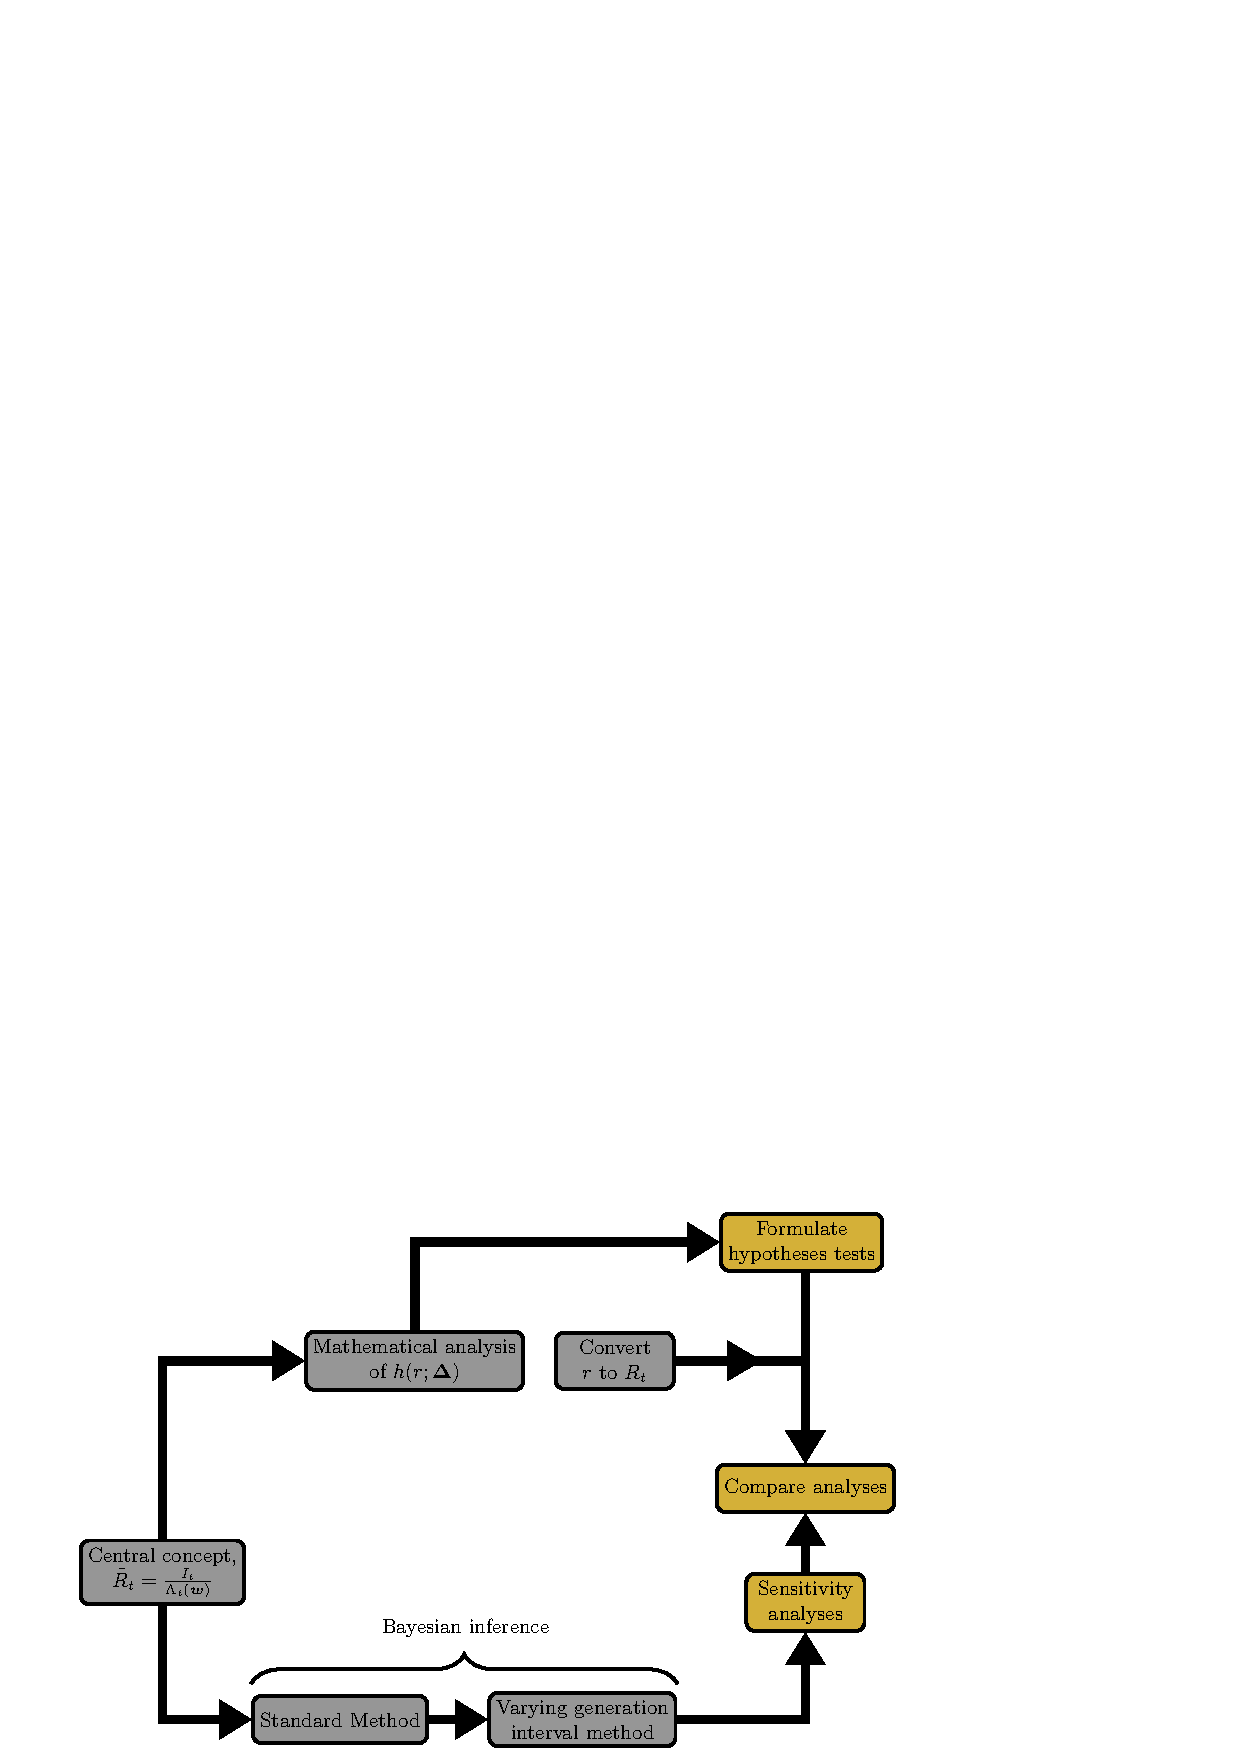
\includegraphics[clip, trim=1.3cm 0cm 1.3cm 0cm,width=\linewidth]{Figures/methods_results.pdf}
\captionof{figure}{}
\label{fig:Methods_and_Results}
\end{figure} 

\subsection{Pre-existing procedures}\label{sect:Cori_Method}
With regards to data, the procedure requires an incidence time series, $\{ I_0, I_1, \cdots I_t \}$ and a single generation interval, $\boldsymbol{w}$. The user must also provide a $\tilde{R}_t \sim \mathrm{Gamma}$ prior distribution, which we will take to be a $\mathrm{Gamma}(1, 5)$ for the remainder of the report. Using a Bayesian framework, the output is a sequence of $\tilde{R}_t \sim \mathrm{Gamma}$ posteriors, from which we can plot the mean and $95 \%$ confidence intervals.\\

The concept enabling $R_t$ inference is simple and best described via figure \href{fig:R_t_Inference_Schematic} illustrating a simple example. If the generation time interval is known, and the dates that each infected person became infected is known, we can calculate $R_t$. Counting back the data and generation time probabilities from Thursday (see top right of figure \ref{fig:R_t_Inference_Schematic}), we can determine how many new infections we expect on Thursday (given each person infects one person) in the following way:
\begin{align*}
\mathbb{E}[I_t|R_t=1] &= w_1 \times I_{\text{Wed}} + w_2 \times I_{\text{Tue}} + w_3 \times I_{\text{Mon}}\\
&= 0.2 \times 1 + 0.5 \times 2 + 0.3 \times 1\\
&= 1.5.
\end{align*}
We can therefore take the ratio of $I_{\text{Thu}}$ and $\mathbb{E}[I_t|R_t=1]$ to give
\begin{align*}
R_t &= \frac{I_{\text{Thu}}}{\mathbb{E}[I_t|R_t=1]}\\
&= 1/1.5\\
&= 0.667 \text{ (3 s.f)}
\end{align*}

\begin{minipage}{0.95\linewidth}
\centering
$R_t$ inference visualised via $\boldsymbol{I}_{t-1} \cdot \mathrm{flip}(\boldsymbol{w})$
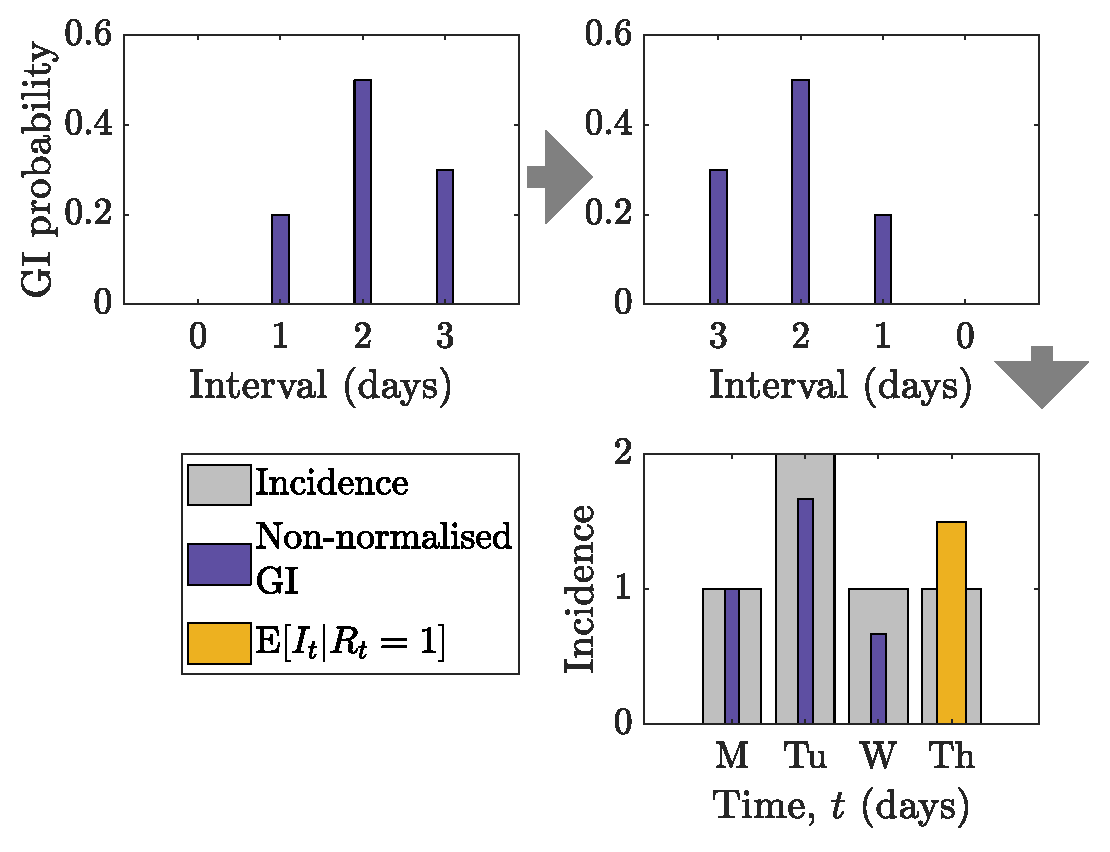
\includegraphics[width=\linewidth]{Figures/R_t_Inference_Schematic.eps}
\captionof{figure}{A variety of transformations from an original serial interval.}
\label{fig:R_t_Inference_Schematic}
\end{minipage} 
\textbf{define bold It vector}
In general, we can write

\begin{align*}
\tilde{R}_t &= \frac{I_t}{\Lambda_t(\boldsymbol{w})} \text{, where}\\
\Lambda_t(\boldsymbol{w}) &= \sum_{i=1}^N w_i \cdot I_{t-i}.
\end{align*}
It follows that
\begin{align*}
\mathbb{E}[I_t |R_t, \boldsymbol{w}, \boldsymbol{I}_{t-1}] &= R_t \Lambda_t(\boldsymbol{w})
\end{align*}
and if we also assume that $I_t$ evolves according to a Poisson process \textbf{MEET}, then
\begin{align*}
 I_t|R_t\ \boldsymbol{w}, \boldsymbol{I}_{t-1} &\sim \mathrm{Poi}(R_t \cdot \Lambda_t(\boldsymbol{w}))\\
\implies \mathbb{P}(I_t = i | R_t, \boldsymbol{w}, \boldsymbol{I}_{t-1}) &= \frac{e^{-R_t\Lambda_t}(R_t\Lambda_t)^i}{i!}
\end{align*}

With this model framework, we can now consider the likelihood of the time series. If we make the assumption that $R_t$ is constant over a time-window $(t-\tau +1, t)$, the following holds from our previous statement

\begin{align*}
\mathbb{P}(I_t=i_t, I_{t-1}=i_{t-1}, &\cdots I_{t-\tau +1} = i_{t-\tau +1}|R_t, \boldsymbol{w})\\ 
&= \prod_{k=t-\tau+1}^t \frac{e^{-R_t \Lambda_k}(R_t \Lambda_k)^{i_k}}{i_k!}
\end{align*} 
If we assume a $\mathrm{Gamma}$ prior for $R_t$, then we know this will be a conjugate prior to a Poisson likelihood. Therefore, using a Bayesian framework:

\begin{align*}
\mathbb{P}(R_t|I_t&=i_t, I_{t-1}=i_{t-1}, \cdots I_{t-\tau +1} = i_{t-\tau +1}, \boldsymbol{w})\\ 
&\propto \mathbb{P}(I_t=i_t, I_{t-1}=i_{t-1}, \cdots I_{t-\tau +1} = i_{t-\tau +1} \boldsymbol{w}) \cdot \mathbb{P}(R_t)\\
&= \Bigg( \prod_{k=t-\tau+1}^t\frac{e^{-R_t \Lambda_k}(R_t \Lambda_k)^{i_k}}{i_k!} \Bigg) \cdot \Bigg(\frac{R_t^{a-1}e^{-\frac{R_t}{b}}}{\Gamma(a)b^a} \Bigg) \\
&\propto R_t^{a-1+\sum_{k=t-\tau+1}^t i_k}\mathrm{exp}\Big( -R_t \Big( \sum_{k=t-\tau+1}^t \Lambda_k(\boldsymbol{w})+\frac{1}{b}\Big)\Big).
\end{align*}
This implies that the updated shape and scale parameters, $a'$ and $b'$ are

\begin{align*}
    a' &= a+\sum_{k=t-\tau+1}^t i_k\\
    b' &= \frac{1}{\sum_{t-\tau+1}^t \Lambda_k(\boldsymbol{w})+1/b}
\end{align*}
where $a$ and $b$ are the shape and scale parameters of the $\mathrm{Gamma}$ distributed prior for $R_t$.\\

The numerical analysis involves inferring the $R_t$ estimate, $\tilde{R}_t$ when the data has been synthetically generated from a Poisson process with the `true $R_t$' fixed. An important feature to clarify is that the confidence intervals for these estimates will inevitably become very narrow. This is our synthetic data will be less susceptible to random fluctuations for larger and larger incidence numbers, and in real world data this is not guaranteed to occur. An example is given in figure \ref{fig:Trivial_Estimate_Zoom}:

\begin{minipage}{0.95\linewidth}
\centering
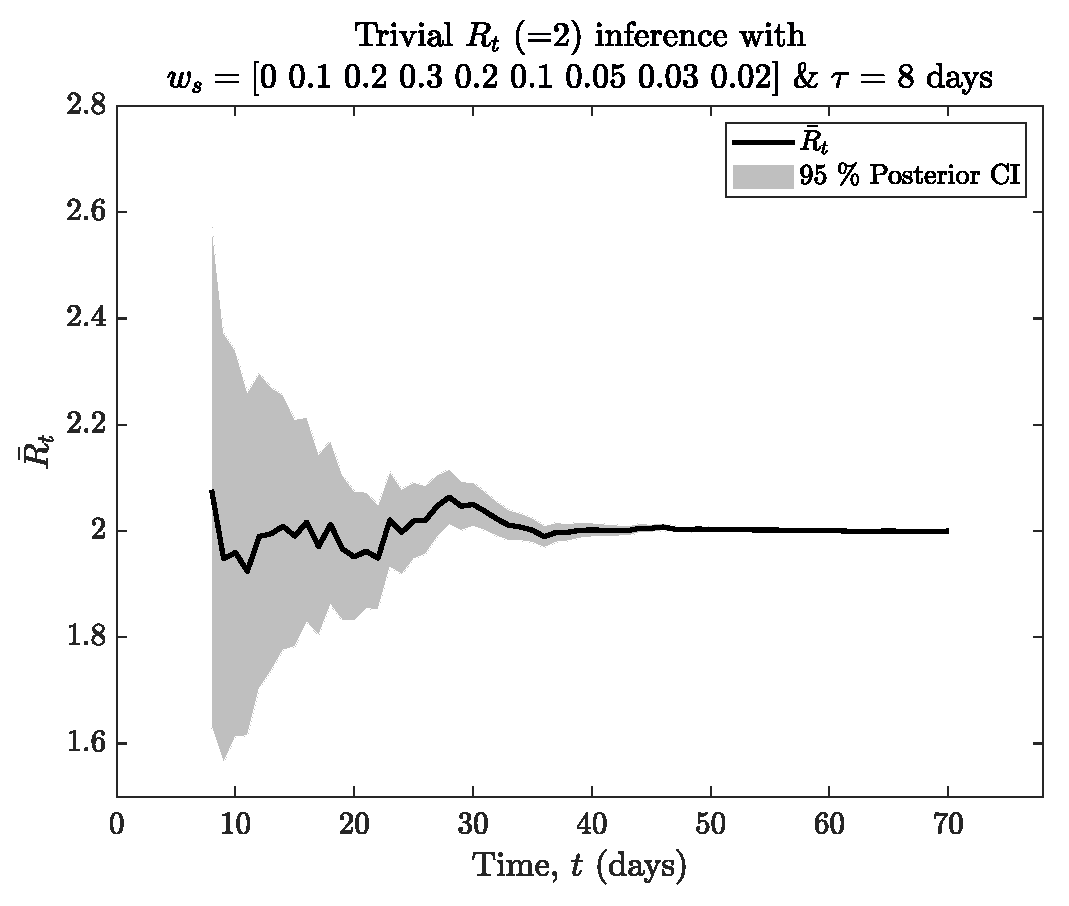
\includegraphics[width=\linewidth]{Figures/Trivial_Estimate_CI_Zoom.eps}
\captionof{figure}{Trivial $R_t$ inference with $\boldsymbol{w} = [0.1, 0.2, 0.3, 0.2, 0.1, 0.05, 0.03, 0.02]$ and $R_t=2$.}
\label{fig:Trivial_Estimate_Zoom}
\end{minipage}  

\textbf{Example features}
\subsection{Procedure adjusted for time-varying generation intervals}\label{sect:Update_method}

Now that we have outlined the standard method for $R_t$ inference, we can subtly alter the method to account for time-varying generation intervals. In theory, we could envisage the generation interval changing each day\footnote{In practice, we will only consider one change to the generation interval but it is helpful to have a generic formula.} so that instead of a vector, $\boldsymbol{w}$ representing the serial interval, we have a generation matrix, $\boldsymbol{W}$, where we denote $\boldsymbol{W}^j$ as the generation interval for the $j$\ts{th} day of the outbreak. We therefore have the exact same shape parameter update but the scale parameter becomes

$$ b' = \frac{1}{\sum_{t-\tau+1}^t \Lambda_k(\boldsymbol{W}^k)+1/b}.$$

\subsection{Notation and techniques and for analysing the affect of a single change in generation interval on $R_t$ inference}\label{sect:Method_Analysis}

The focus of this report is to develop the understanding of how $R_t$ inference depends on whether or not the generation interval has been updated. Our mathematical analysis outlines the role of key parameters, particularly with regards to the generation interval. This mathematical analysis has informed the hypotheses listed in \ref{sect:Hypotheses} and in order to be tested numerically, we must also introduce various numerical parameters. Table \ref{table:table_1} lists all the necessary variables and parameters that the remainder of the report will refer to frequently.

\begin{table}[htbp]
\centering
\begin{tabular}{|c||c|} \hline\hline
Parameter & Description \\ \hline
$R_t$ & \makecell{True time-dependent reproduction number, \\ involved in synthetically generating the incidence data} \\ \hline

$r$ & Epidemic growth rate \\ \hline

$I_t, I_t(r)$ & \makecell{Incidence data (synthetic, theoretical or \\ real),i.e. number of new cases at time $t$. \\ When $I_t$ is modelled theoretically, it is \\ convenient to view it as a function of $r$}.\\ \hline

$\tilde{R}_t$ & \makecell{Generic inferred time- \\ dependent reproduction number} \\ \hline

$\tilde{R}_t^o$ & \makecell{Inferred time-dependent reproduction \\ number, using the un-updated \\ generation interval } \\ \hline

$\tilde{R}_t^a$ & \makecell{Inferred time-dependent reproduction \\ number, using the updated generation interval } \\ \hline

$\boldsymbol{w}$ & \makecell{Generic generation interval distribution,\\ i.e. $w_i = \mathbb{P}(\text{time delay between}$ \\ $\text{infection of infector and infectee}=i)$ \footnote{We model $\boldsymbol{w}$ as the generation interval distribution, indicating that we model the probability of the infector infecting an infectee on the same day as their infection is 0. Additionally, the model is more frequently applied when $\boldsymbol{w}$ is the serial interval. Discuss this in biases section!}} \\ \hline

$\boldsymbol{w}^o$ & \makecell{Un-updated generation interval distribution, \\ involved in synthetically generating incidence \\ data before $T_i$ and inferring both $\tilde{R}_t^o$ \\ (for all time) and $\tilde{R}_t^a$ (before $t=T_i$)}\\ \hline

$\boldsymbol{w}^a$ & \makecell{Updated generation interval \\ distribution, involved in synthetically \\ generating incidence data after \\ $T_i$ and inferring $\tilde{R}_t^a$ (after $t=T_i$)}\\ \hline

$N$ & \makecell{Length of $w$, i.e. maximum number of days \\ for which delay between infection of \\ infector and infection of infectee \\ is modelled to be possible.} \\ \hline

$h(r)$ & \makecell{$\frac{\tilde{R}_t^o}{\tilde{R}_t^a} = \frac{\sum_{i=1}^{N}I_{t-i}(r)w_i^a}{\sum_{i=1}^{N}I_{t-i}(r)w_i^o}$, i.e. the ratio \\ of the two inferred reproduction numbers} \\ \hline

$\boldsymbol{\Delta}$ & \makecell{Change in generation interval after \\ the update, $\boldsymbol{w^a}-\boldsymbol{w}^o$} \\ \hline

$\alpha = \alpha(\boldsymbol{\Delta})$ & \makecell{Number of sign changes in the sequence $\Delta_i$ \\ for $\delta=1, 2, \cdots N$, e.g. $\alpha([0.1, -0.2, 0.1])=2$} \\ \hline

$\beta = \beta(\boldsymbol{w}^{\{o, a\}})$ & $\frac{w_1^a}{w_1^o}$ \\ \hline

$\mu_{\boldsymbol{\Delta}}$ & $\mathbb{E}[\boldsymbol{\Delta}] = \sum_{i=1}^Ni\Delta_i$ \\ \hline

$\sigma^2_{\boldsymbol{\Delta}}$ & $\mathrm{Var}[\boldsymbol{\Delta}] = \sum_{i=1}^N(i-\mu_{\boldsymbol{\Delta}})^2$ \\ \hline

$T_i$ & \makecell{Time at which true serial interval changes \\ from $\boldsymbol{w}^o$ to $\boldsymbol{w}^a$} \\ \hline

$T_e$ & Time at which simulation ends \\ \hline
 $\tau$ & ? \\\hline\hline
\end{tabular}
\caption{}
\label{table:table_1}
\end{table}

\subsubsection{Derivation of the relative inference quantifier, $h(r)$}

The method for our mathematical and numerical analysis of how $R_t$ may be over/under-estimated with un-updated generation intervals is centred around the quantity we denote $h$. Since we have introduced the necessary notation in sections \ref{sect:Cori_Method} and \label{sect:Update_Method}, we derive its form here:

\begin{align*}
    \tilde{R}_t^o = \frac{I_t}{\Lambda_t(\boldsymbol{w}^o)} &\text{, }
    \tilde{R}_t^a = \frac{I_t}{\Lambda_t(\boldsymbol{w}^a)}\\
    h&= \frac{\tilde{R}_t^o}{\tilde{R}_t^a} = \frac{\Lambda_t(\boldsymbol{w}^a)}{\Lambda_t(\boldsymbol{w}^o)}\\
    &= \frac{\sum_{i=1}^Nw_i^aI_{t-i}}{\sum_{i=1}^Nw_i^oI_{t-i}}.
\end{align*}

Since $\Lambda_t$ is actually a function of the time series of $\{I_0, I_1, \cdots , I_t \}$, we will show in section \ref{sect:Results} that this time series is a function of $r$. We will also show that the key characteristics of $h(r)$ are properties of $\boldsymbol{\Delta}$ and therefore

\begin{mdframed}
\begin{equation}\label{eq:Key_Equation}
   h(r; \boldsymbol{\Delta}) = \frac{\tilde{R}_t^o}{\tilde{R}_t^a} = \frac{\sum_{i=1}^Nw_i^aI_{t-i}}{\sum_{i=1}^Nw_i^oI_{t-i}}
\end{equation}
\end{mdframed}

Using equation (\ref{eq:Key_Equation}), we can summarise how $h(r)$ informs whether or not time-varying generation intervals affect reproductive number inference:\\
\begin{table}[h]
\centering
\begin{tabular}{c l}
Relative inference quantifier & $\tilde{R}_t^o$ estimation bias \\
\hline
$h(r) < 1$ & under-estimate \\
$h(r) = 1$ & none \\
$h(r) > 1$ & over-estimate \\ \hline
\end{tabular}
\label{table:table_2}
\end{table}

\subsubsection{The relationship between the epidemic growth rate, $r$ and the time-dependent reproduction number, $R_t$}

$h(r)$ will quantify the ratio of an un-updated $R_t$ inference to an updated $R_t$ inference, however we will be unable to verify our hypotheses in section \ref{sect:Results} without being able to translate $r$ to $R_t$. We adjust the empirical distribution relationship between $r$ and $R_t$ in \cite{Wallinga-Lipsitch} to give 
\begin{align*}\label{eq:r_to_R}
  R_t = \frac{r}{\sum^N_{i=1}w_i \cdot(e^{-r(i-1/2)} - e^{-r(i+1/2)})}
\end{align*}
by taking $a_i = i+1/2$. 
\subsection{Verification of Hypotheses}
The hypotheses are listed in \ref{sect:Hypotheses}, all of which relate to the shape of $h(r)$. Verification of the hypotheses will be mathematical in nature, and we will employ standard mathematical techniques to prove the claims of these hypotheses. Additionally, we support the mathematical arguments with numerical tests to further convince the reader that the hypotheses have not been dis-proven.


The results will largely be in the format of sensitivity analyses, where we plot a characteristic of $\boldsymbol{\Delta}$ on the $y$-axis and the `true $R_t$' on the $x$-axis. The colour scheme for the sensitivity analyses correspond to some error measure for how $\tilde{R}_t$ was re-inferred in comparison to the true $R_t$, for a given characteristic of $\mu_{\boldsymbol{\Delta}}$. This means each `square' on the sensitivity analysis corresponds to an error measure for some inference comparison. To illustrate this for a simple example, we present figures \ref{fig:Constant_R_Disc_Serial_0} and \ref{fig:Constant_R_Disc_Serial_1}.

\begin{minipage}{0.95\linewidth}
\centering
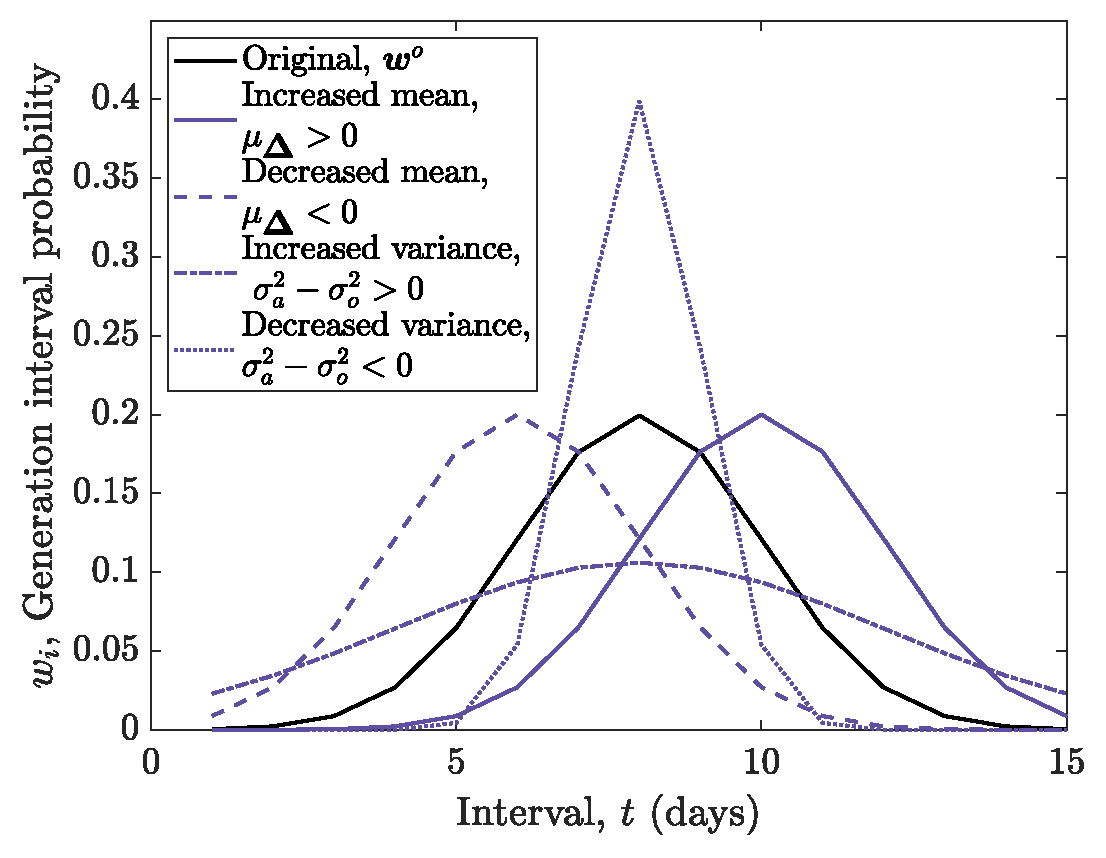
\includegraphics[width=\linewidth]{Figures/Report_Constant_R_Disc_Serial_0.eps}
\captionof{figure}{A variety of transformations from an original serial interval.}
\label{fig:Constant_R_Disc_Serial_0}
\end{minipage}  
  
\begin{minipage}{0.95\linewidth}
\centering
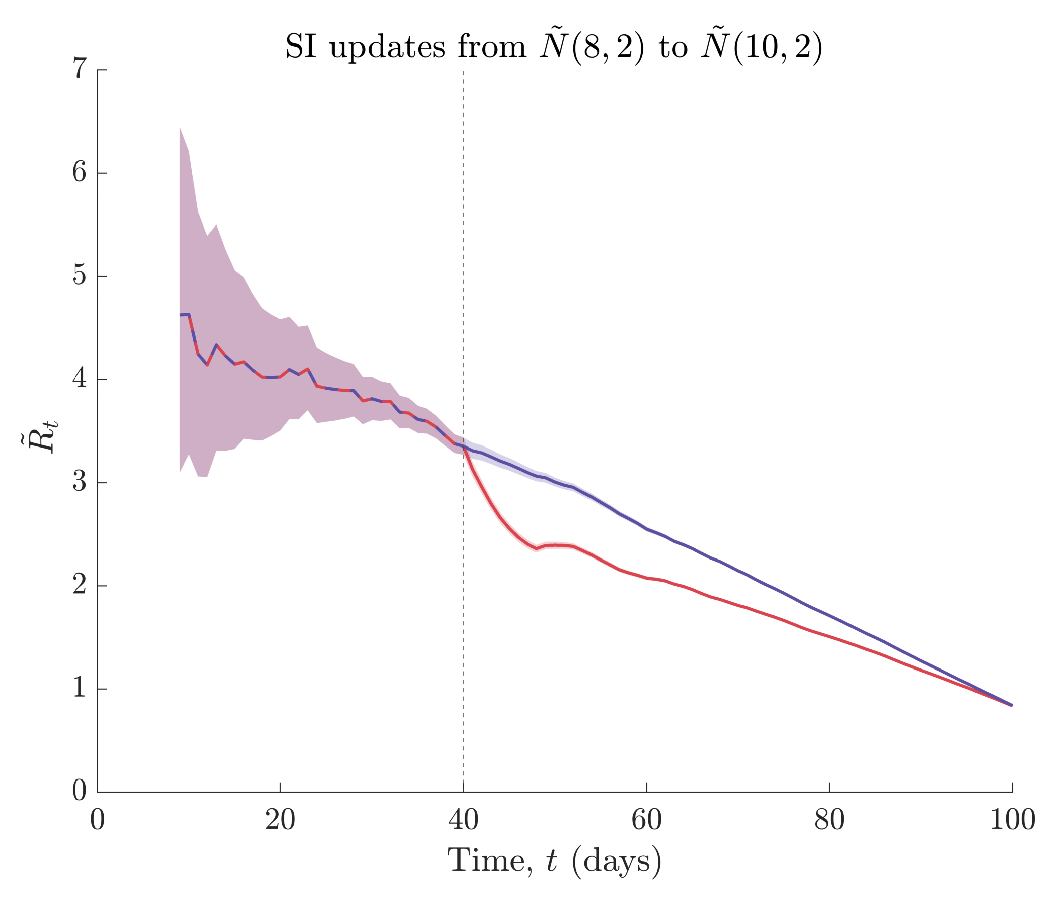
\includegraphics[width=\linewidth]{Figures/Report_Constant_R_Disc_Serial_1.eps}
\captionof{figure}{This figure is uses the same inference technique discussed in the Methods section, except we are now comparing two re-inferences.)}
\label{fig:Constant_R_Disc_Serial_1}
\end{minipage}

Figure \ref{fig:Constant_R_Disc_Serial_1} shows that there is a change in the synthetic generation of data at time $T_i=40$ days. The blue time-series incorporates this update into the inference, whereas the red time-series does not (and infers using the old serial interval). As we can see, the inference for the un-updated $\tilde{R}_t$ is consistently less than the updated $\tilde{R}_t$ inference. We can summarise a feature of this figure by recording an error in the inference comparison. This error is then what is colour-encoded in the sensitivity analysis figures \textbf{later on}. Note that 
\begin{enumerate}
    \item in order for the error to be easily compared to the hypotheses, we should let negative errors correspond to under-estimates and positive errors correspond to over-estimates.
    \item we may require multiple simulations (over different seeds) to generate robust sensitivity analyses. It may also suffice to remove stochasticity from the Poisson process and instead plot the expectation.
\end{enumerate}
\\

H\ref{hyp:first} is proven rigorously by considering the existence of solution(s) to $\boldsymbol{v}(r) \cdot \boldsymbol{\Delta}=0$, where

  \begin{align*}
    \boldsymbol{v}(r) &= \begin{pmatrix}
           e^{-r} \\
           e^{-2r} \\
           \vdots \\
           e^{-Nr}
         \end{pmatrix}.
  \end{align*}

We then use sensitivity analyses to show that the solution (once converted from $r$ to $R_t$ using [\ref{eq:r_to_R}]) does align with what we show numerically.

H\ref{hyp:second} requires new notation

H\ref{hyp:thirda}H\ref{hyp:thirdf} will be argued non-rigorously via diagrams and rely heavily on $h(r)$ being a continuous function of $r$. The 3D plots will be particularly illuminating numerically.\\



H\ref{hyp:fourth} is the only hypothesis, which is not supported by numerical simulations. We suppose that the $h(r)$ is not bounded in the manner described and use a water-tight to deduce a contradiction, proving that the assumption must be false, i.e. \textit{reductio ad absurdum}.

% For H\ref{hyp:first} and H\ref{hyp:seconda}-\ref{hyp:secondf}, we run 100 simulations for each combination of $R_t \in (0.1, 6)$ and $\mu_{\boldsymbol{\Delta}} \in (-0.3, 0.3)$ [for $\delta=2$] or $(-1, 1)$ [for $\delta=1$]. For H\ref{hyp:third}, we run 1 simulation for each combination of $\mu_{\boldsymbol{\Delta}} \in (-0.3, 0.3)$ and $R_t \in (0.1, 6000)$ [we only investigate for $\delta=2$]. To test H\ref{hyp:first} when $\delta=1$, we need to confirm, from the sensitivity analysis, that there is no (non-trivial) parameter space where the error measure is 0 (other than the trivial $r=0$ case). This will confirm that $h(r)=1$ has only one solution. To test the same hypothesis when $\delta=2$ we need to confirm, from the sensitivity analysis, that there is a region where the error measure is zero (In reality we can only check that the absolute error gets very small.). Even more specifically we should be able to numerically solve $\boldsymbol{\Delta} \cdot \boldsymbol{v}(r^*)=0$ for each value of $\mu_{\boldsymbol{\Delta}}$, convert $r^*$ to $R_t^*$ (using \textbf{appendix}) and then plot the resulting locus of points on top of the sensitivity analysis. This region should be exactly where the sensitivity analysis suggests the error is becoming negligible. Confirming \textbf{or not word} H\ref{hyp:seconda}-\ref{hyp:secondf} can use the same sensitivity figures as that used in H\ref{hyp:first} but instead we fix a value of $\mu_{\boldsymbol{\Delta}}$ and follow an error sensitivity (not taking the absolute value), i.e. if we are investigating \ref{hyp:seconda}, we would expect to find that the error term is positive when $r>0$ but negative when $r<0$. We can also trace up and down the sensitivity to see if the behaviour switches for relevant values of $\mu_{\boldsymbol{\Delta}}$. 
Testing H\ref{hyp:second} requires some introduction of notation. Let $$h_{i,j} = h(j=R_t; i = \mu_{\boldsymbol{\Delta}})\footnote{Note that we are being quite flexible over whether $h$ is a function of $R_t$ or $r$.},$$
which will also form each `square' on the sensitivity analysis for H\ref{hyp:second}. We can also define the vector
\begin{align}
    \boldsymbol{h}(R_t) &= \begin{pmatrix}
           h_{\mu_1, R_t} \\
           h_{\mu_2, R_t} \\
           \vdots \\
           h_{\mu_M, R_t}
         \end{pmatrix},
  \end{align}
where $\{\mu_1, \cdots , \mu_M\}$ is the set of $\mu_{\Delta}$s which form the characteristic of $\Delta$ we wish to investigate. We also define $\beta$ such that $$beta_i = \frac{w_1^a}{w_1^o},$$
where $w_1^a$ is the $i$\ts{th} updated serial interval of interest. We may now define the function $$ g(R_t) = (\boldsymbol{h}(R_t)-\boldsymbol{w})\cdot \boldsymbol{1}/||\boldsymbol{w}||_1,$$
where $1$ is the vector of 1s and $||\cdot||_1$ is the so-called Taxicab norm (the sum of the absolute values of the vector). This definition is equivalent to $$ g(R_t) = \frac{\sum_{i=1}^M h(R_t, \mu_i)-w_i}{\sum_{i=1}^M w_i}.$$ Given our definition of $g(R_t)$ and our hypothesis H\ref{hyp:second}, we would expect that $g(R_t) \rightarrow 0$ as $R_t \rightarrow \infty$ and forms our verification method for H\ref{hyp:second}. We attempt to show this by plotting $g(R_t)$, fitting a suitable curve, and confirming whether or not this curve tends to 0 for large $R_t$.\\

\subsection{Choice of $\boldsymbol{\Delta}$}

For all three hypotheses, we must predetermine a range of $\Delta$ vectors. The hypotheses will indicate that there are only a few characteristics of $\Delta$ that are significant for $R_t$ estimation. This means there is an infinite choice of $\Delta$ vectors. We considered two options for $\Delta$ generation:
\begin{enumerate}
    \item Generating $w^a$ vectors from a given probability mass distribution (with pre-decided mean and variance) and computing the difference $\Delta = w^a-w^o$.
    \item Generating $\Delta$ directly by pre-deciding $\mu_{\Delta}$ and $\sigma^2_{\Delta}$. This requires deciding on a `form' for $\Delta$ and using matrix algebra to calculate a matrix, which contains the $\Delta$ vectors.
\end{enumerate}
We decided to opt for option 2 since option 1 requires limiting oneself to a specific probability mass function. It is also difficult to both pre-determine mean and variance values, as well as assuring that the $\delta$ value remains the same throughout all the $\Delta$ vectors (for common probability mass distributions).\\

Since the `form' of $\Delta$ depends on whether $\delta=1$ or $\delta=2$, we calculated $\Delta$ in two different ways for each method. There are numerous ways to do this but we opted to take the following forms for simplicity:

\begin{enumerate}
    \item $\Delta_i$ is linear in $i$ when  $\delta=1$
    \item $\Delta_i$ is quadratic in $i$ when $\delta=2$
\end{enumerate}
These forms of $\Delta$ enable one or two sign-changes \footnote{Note that because $\sum_{i=1}^N \Delta_i=0$, the linear form of $\Delta$ necessarily has one root, where as there could be one \textit{or} two sign changes for the quadratic form.}. Sections \ref{sect:delta_gen_1} and \ref{sect:delta_gen_2} state the generation methods, the details of the derivations are given in \textbf{Appendix}.

\subsubsection{$\Delta$ generation for $\delta=1$}\label{sect:delta_gen_1}

We will generate a matrix with entries
\begin{align}\label{eq:Delta_Matrix}
 \boldsymbol{\hat{\Delta}}_{i, j} = a_ji+b_j,
\end{align}
 where $i=1, \ldots, N$ ($N$ is the length of the serial interval) and $j = 1, \ldots , M$ ($M$ is the number of serial intervals that we are generating). There are two rules for $\hat{\Delta}$ as a matrix:
\begin{align}
    \boldsymbol{\hat{\Delta} 1} &= \boldsymbol{0}\label{eq:cons_of_prob_1}\\
    \boldsymbol{\hat{\Delta} i} &= \boldsymbol{\mu}\label{eq:mean_1},
\end{align}
where $\boldsymbol{1}$ is the vector of 1s of length $N$,
\begin{align}
    \boldsymbol{i} &= \begin{pmatrix}
           1 \\
           2 \\
           \vdots \\
           N
         \end{pmatrix}
  \end{align}
  
  and $\boldsymbol{\mu}$ is the vector of $\mu_\boldsymbol{\Delta}$ values. Combined with our definition of $\boldsymbol{\hat{\Delta}}$ in \ref{eq:Delta_Matrix}, we can show that
  \begin{align*}
      \boldsymbol{x} = \boldsymbol{B}_l^{-1}\boldsymbol{c}_l,
  \end{align*}
where

\begin{align*}
      \boldsymbol{x} &= \begin{pmatrix}
           a_1 \\
           b_1 \\
           a_2 \\
           b_2 \\
           \vdots \\
           a_N \\
           b_N
         \end{pmatrix},
         \boldsymbol{c}_l = \frac{6}{N(N+1)}\begin{pmatrix}
           0 \\
           \mu_1 \\
           0 \\
           \mu_2 \\
           \vdots \\
           0 \\
           \mu_N
         \end{pmatrix} \text{ and }\\
         \\
         \boldsymbol{B}_l &=
         \begin{pmatrix}
\boldsymbol{A}_l & \boldsymbol{0} & \cdots &\boldsymbol{0} & \boldsymbol{0} \\
\boldsymbol{0} & \boldsymbol{A}_l & \cdots & \boldsymbol{0} & \boldsymbol{0} \\
\vdots & \vdots & \ddots & \vdots & \vdots \\
\boldsymbol{0} & \boldsymbol{0} & \cdots & \boldsymbol{A}_l & \boldsymbol{0} \\
\boldsymbol{0} & \boldsymbol{0} & \cdots & \boldsymbol{0} & \boldsymbol{A}_l
\end{pmatrix} \text{, where}\\
\\
\boldsymbol{A}_l &=
\begin{pmatrix}
N+1 & 2 \\
2N+1 & 3
\end{pmatrix}.
\end{align*}
This expression for $\boldsymbol{x}$ can then be fed back into equation (\ref{eq:Delta_Matrix}).
The linear $\Delta$ implemented in our numerical testing of various hypotheses is given in figure \ref{fig:Linear_Delta}

\begin{minipage}{0.95\linewidth}
\centering
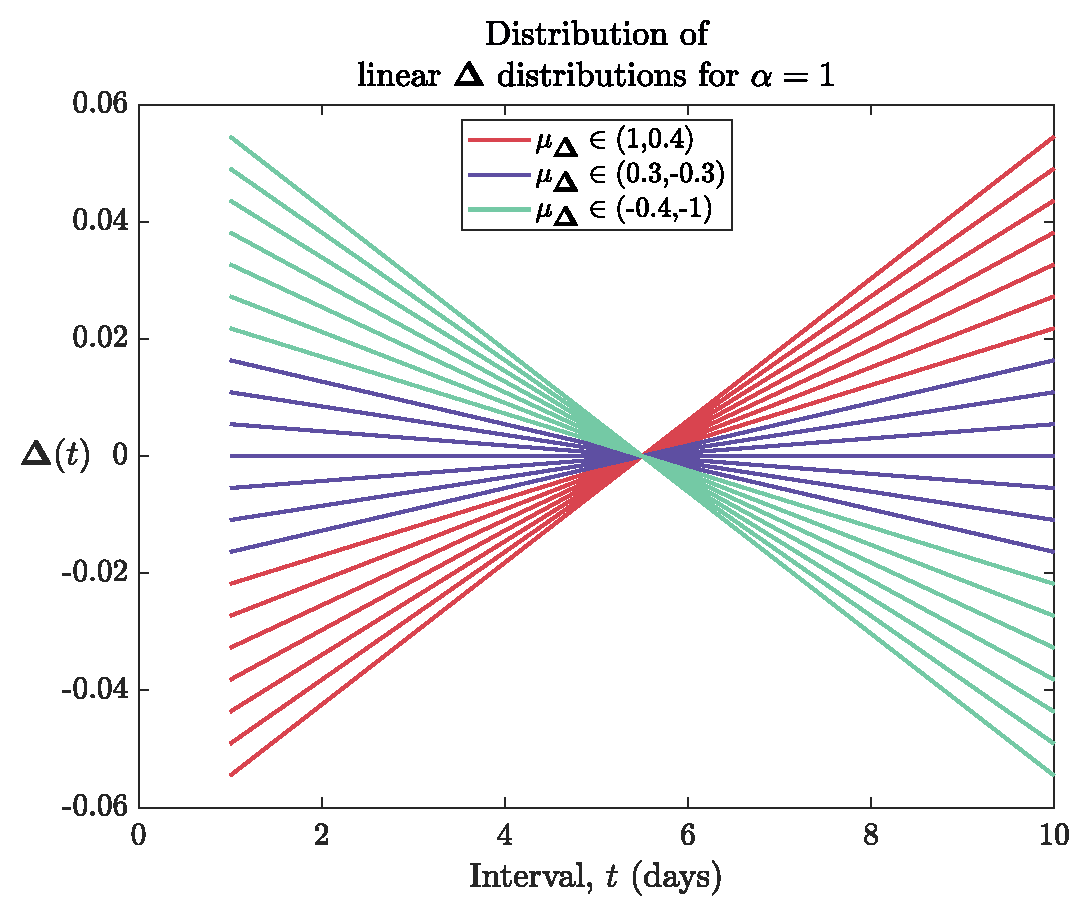
\includegraphics[width=\linewidth]{Figures/Linear_Delta.eps}
\captionof{figure}{)}
\label{fig:Linear_Delta}
\end{minipage}

\subsubsection{$\Delta$ generation for $\delta=2$}\label{sect:delta_gen_2}

Here, we use the same method for $\Delta$ generation as in the $\delta=1$ case. But instead we will not use block matrices in our final expression, and will think of each $\Delta$ in isolation illustrating to the reader that such a large matrix is not necessary.
We consider $$\Delta_i = k_1+k_2i+k_3i^2$$ for a given value of $\mu$ and $\sigma^2$ and then repeat for a different set of $k_1$, $k_2$, $k_3$.\\
We can compute 
\begin{align*}
    \boldsymbol{k} = \begin{pmatrix}
           k_1 \\
           k_2 \\
           k_3
         \end{pmatrix},
\end{align*}
Since the quadratic form takes three unknowns, we now require three rules for $\Delta$ (leaving only two will leave the solution \textit{under-determined}):
\begin{align}
    \sum_{i=1}^N\Delta_i &= 0 \label{eq:cons_of_prob_2}\\
    \sum_{i=1}^N\Delta_i \cdot i &= \mu_{\Delta} \label{eq:mean_2}
    \sum_{i=1}^N\Delta_i \cdot i^2 &= \mu_{\Delta}^2 + \sigma_{\Delta}^2 \label{eq:variance_Delta},
\end{align}

  Combined with our definition of $\Delta$ given above, we can show that
\begin{align*}
\boldsymbol{k} &= \boldsymbol{A}_q^{-1}\boldsymbol{c}_q,\\\text{where} \\
\boldsymbol{A}_q &= 
\begin{pmatrix}
N & \frac{N^2+N}{2} & \frac{2N^3+3N^2+N}{6}\\
\frac{N^2+N}{2} & \frac{2N^3+3N^2+N}{6} & \frac{(N^2+N)^2}{4}\\
\frac{2N^3+3N^2+N}{6} & \frac{(N^2+N)^2}{4} & \frac{6N^5+15N^4+10N^3-N}{30}
\end{pmatrix}\\
\text{and }
\boldsymbol{c}_q &= \begin{pmatrix}
0 \\
\mu_{\Delta}\\
\mu_{\Delta}^2 +\sigma_{\Delta}^2
\end{pmatrix}.
\end{align*}
Once again, these values of $k_1, k_2, k_3$ can be fed back in to generate $\Delta$. The difference to the previous approach for $\delta=1$ is that we must loop this calculation over the number of $\Delta$ vectors we wish to generate, $M$. The quadratic $\Delta$ implemented in our numerical testing of hypotheses relating to $\delta=2$ is given in figure \ref{fig:Quadratic_Delta}.

\begin{minipage}{\linewidth}
\centering
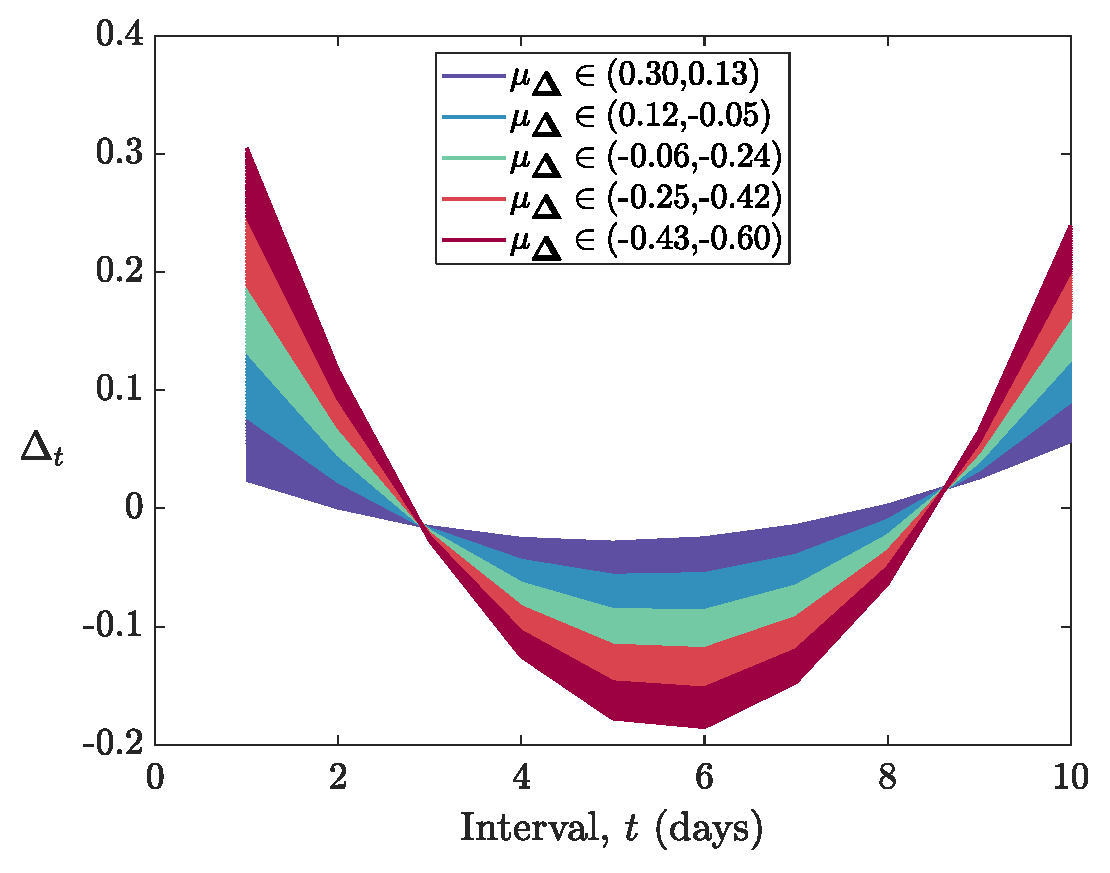
\includegraphics[width=\linewidth]{Figures/Quadratic_Delta.eps}
\captionof{figure}{}
\label{fig:Quadratic_Delta}
\end{minipage}

\section{Results}\label{sect:Results}

\subsection{Hypotheses}\label{sect:Hypotheses}

We propose the following hypotheses:

\begin{hyp}[H\ref{hyp:first}] \label{hyp:first}
When $\delta=1$ ($\delta=2$) there is exactly one (are exactly two) solution(s) to $h(r; \boldsymbol{\Delta}))=1$, namely $r=1$ (and the solution to $\boldsymbol{\Delta} \cdot \boldsymbol{v}(r^*)=0$).
\end{hyp}
\begin{hyp}[H\ref{hyp:second}]
\label{hyp:second}
\begin{align*}
    \lim_{r\rightarrow \infty}h(r; \boldsymbol{\Delta})&=\beta \text{, and} \\
    \lim_{r\rightarrow -\infty}h(r; \boldsymbol{\Delta})&=1
\end{align*}
where $\beta$ = $w_1^a/w_1^o$.
\end{hyp}
The following sub-hypotheses concern the behaviour of $h(r)$ for finite $r$, i.e. that it is the same as figures \ref{fig:Delta_Eq_1} and \ref{fig:Delta_Eq_2} (with regards to whether $h(r) \gtrless 1$) \footnote{Reference to the figures mentioned will probably be easier to interpret the results with, as opposed to these wordy hypotheses!}.
\begin{subhyp}
\begin{hyp}[H\ref{hyp:thirda}]
\label{hyp:thirda}
When $\delta = 1$ \& $\mu_{\boldsymbol{\Delta}}<0$ we have $h(r)>1$ for $r>0$ and $h(r) \in (0,1)$ for $r<0$.
\end{hyp}
\begin{hyp}[H\ref{hyp:thirdb}]
\label{hyp:thirdb}
When $\delta = 1$ \& $\mu_{\boldsymbol{\Delta}}>0$ we have $h(r) \in (0, 1)$ for $r>0$ and $h(r)<1$ for $r<0$.
\end{hyp}
\begin{hyp}[H\ref{hyp:thirdc}]
\label{hyp:thirdc}
When $\delta = 2$, $\mu_{\boldsymbol{\Delta}}<0$ \& $w_1^a<w_1^o$, we have $r^*>0$ and $h(r) \in (0,1) \forall r \notin (0, r^*)$. $h(r)>1$ for $r \in (0, r^*)$.
\end{hyp}
\begin{hyp}[H\ref{hyp:thirdd}]
\label{hyp:thirdd}
When $\delta = 2$, $\mu_{\boldsymbol{\Delta}}<0$ \& $w_1^a>w_1^o$, we have $r^*<0$ and $h(r)>1 \forall r \notin (r^*, 0)$. $h(r) \in (0,1)$ for $r \in (r^*, 0)$.
\end{hyp}
\begin{hyp}[H\ref{hyp:thirde}]
\label{hyp:thirde}
When $\delta = 2$, $\mu_{\boldsymbol{\Delta}}>0$ \& $w_1^a<w_1^o$, we have $r^*<0$ and $h(r) \in (0,1) \forall r \notin (r^*, 0)$. $h(r) \in (0,1)$ for $r \in (r^*, 0)$.
\end{hyp}
\begin{hyp}[H\ref{hyp:thirdf}]
\label{hyp:thirdf}
When $\delta = 2$, $\mu_{\boldsymbol{\Delta}}>0$ \& $w_1^a>w_1^o$, we have $r^*>0$ and $h(r) >1 \forall r \notin (0, r^*)$. $h(r)\in (0,1)$ for $r \in (0, r^*)$.
\end{hyp}
\end{subhyp}
\begin{hyp}[H\ref{hyp:fourth}]
\label{hyp:fourth}
When $\delta=1$ and $\mu_{\Delta}<0$ ($\mu_{\Delta}>0$) $h(r>0; \boldsymbol{\Delta})$ is bounded above (below) by $w_1^a/w_1^o$. 
\end{hyp}

(Table \ref{table:table_1}  in Section \ref{sect:Methods} will be helpful to the reader in understanding any new notation.)

We present our results by systematically approaching each hypothesis, H\ref{hyp:first}-\ref{hyp:fourth}, providing first the skeleton of any mathematical proofs/arguments before supporting this material with numerical tests. The supporting mathematical analysis is made clearly available in the appendix. The reader should not that these hypotheses are ordered in the way they are since they are contingent on one another so a chronological reading is most suitable. Prior to this analysis, we outline some of the mathematics that is relevant to all of the hypotheses.\\

For this analysis, we shall assume that $I_t$ is `well behaved', i.e. $I_t \sim p+qe^{rt}$ and we will assume that $p$ and $q$ are both positive (although there may be examples where this is not a necessary condition). Combining this assumption with the central concept, \ref{eq:Key_Equation}, we can show that
\begin{equation}\label{eq:Analysis_centre}
    h(r) = \frac{p+qe^{rt}L_a(r)}{p+qe^{rt}L_o(r)},
\end{equation}
where $L$ takes a form analogous to a discrete Laplace transform:
\begin{equation}
L_{\{o, a\}}(x) = \sum_{i=1}^{N}e^{-ix}w_i^{\{o, a\}}.
\end{equation}

\subsection{H\ref{hyp:first} Analysis}

H\ref{hyp:first} concerns solving $h(r; \Delta) = 1$ and the characteristic of $\Delta$, $\alpha$ defined as the number of sign changes in $\Delta$. The appendix shows that this is equivalent to asking for which $r$, $\Delta$ is orthogonal to $\boldsymbol{v}(r)$, where 
\begin{align*}
    \boldsymbol{v}(r) &= \begin{pmatrix}
           e^{-r} \\
           e^{-2r} \\
           \vdots \\
           e^{-Nr}
         \end{pmatrix}.
  \end{align*}

This can further be reduced to finding the roots of the polynomial

\begin{equation}\label{eq:Poly}
    \Delta_1 +\Delta_2 z + \cdots +\Delta_{N}z^{N-1} = 0,
\end{equation}

by letting $z = e^{-r}$ (noting that this forces $z>0$).\\

We now recall a theorem from algebra

\begin{mdframed}\label{Thm:1}
\textbf{Theorem 1: Descartes' Rule of Signs. }\textit{Let $p(x) = a_0x^{b_0} + a_1 x^{b_1}+ \cdots + a_nx^{b_n}$ denote a polynomial with nonzero real coefficients $a_i$, where the $b_i$ are integers satisfying $0\leq b_0 < b_1 < b_2 \cdots < b_n$. Then the number of positive real zeros of $p(x)$ (counted with multiplicities) is either equal to the number of variations in sign in the sequence $a_0, \cdots a_n$ of the coefficients or less than that by an even whole number.}
\end{mdframed}

As a result of this theorem, we reason in the appendix, that the polynomial above can only have $\alpha$ roots (note this only holds for $\alpha=1,2$ and becomes more complex if $\alpha>2$). We also reason that one of these roots is always $z=1$, i.e. $r=0$. However, when $\alpha=2$, there is a non-trivial root of the polynomial.

\subsection{H\ref{hyp:second} Analysis}

\subsection{H\ref{hyp:thirda}-\ref{hyp:thirdf} Analysis}

By considering $\alpha$ (i.e. the number of solutions to $h(r)=1$), how $h'(0)$ depends on $\mu_{\Delta}$ and the limits of $h(r) \rightarrow \pm \infty$, we can determine the general shape of $h(r)$. These sub-hypotheses are detailed so for brevity, we will outline proofs of \ref{hyp:thirda} and \ref{hyp:thirdc} since they will be broadly similar proofs for the remaining for sub-hypotheses.\\

In the appendix, we show that

\begin{equation}
    \mathrm{sgn}\{ h'(0)\} = -\mu_{Delta}
\end{equation}



\subsection{H\ref{hyp:fourth} Analysis}
-----------------------------------


\begin{equation} \label{eq:R_t_ratio}
\frac{\tilde{R}_t^o}{\tilde{R}_t^a} = \frac{\sum_{i=1}^{N}I_{t-i}w_i^a}{\sum_{i=1}^{N}I_{t-i}w_i^o},
\end{equation}
where $N$ is the length of both the original and actual serial intervals (this time the length is not truncated). Note that the quantity in (\ref{eq:R_t_ratio}) is the ratio of \textit{inferred} $R_t$ values and will inform us on whether we are over/under-estimating the reproduction number, and by how much.\\
Let us define both

  \begin{align*}
    \boldsymbol{v}(r) &= \begin{bmatrix}
           e^{-r} \\
           e^{-2r} \\
           \vdots \\
           e^{-Nr}
         \end{bmatrix} \text{ and}\\
         \boldsymbol{\Delta} &= \boldsymbol{w}^a-\boldsymbol{w}^o,
  \end{align*}
  
where $\boldsymbol{w}^o$ and $\boldsymbol{w}^a$ are the original and actual (after the original serial interval is updated) serial intervals respectively.\\
The reader should note that (as we will make clear soon) that $r$ is the \textit{epidemic growth rate} \textbf{find reference}. \footnote{Throughout this analysis, we will refer to both $R_t$ and $r$ interchangeably (the exact relationship has been discussed thoroughly in \cite{Wallinga-Lipsitch}, which we make reference to later) but crucially $R_t>1$ if and only if $r>0$, whilst $R_t<1$ if and only if $r<0$.}
Equation (\ref{eq:R_t_ratio}) shows that we are interested in understanding what happens to $R_t$ inference when the original serial interval is used, instead of the updated (actual) serial interval.\\
Crucially, we note that $\boldsymbol{v}(r)$ is not necessarily orthogonal to $\boldsymbol{\Delta}$. The importance behind this relationship will become clear during this section. \footnote{Discussing the existence of a non-zero $r$ that makes $\boldsymbol{v}(r)$ orthogonal will form a large part of our analysis.}

Suppose we know the following:

\begin{itemize}
    \item whether or not $\mu_a \mathop{\lessgtr} \mu_o $ (and $\sigma_a \mathop{\lessgtr} \sigma_o$ although as we shall see the variance of the interval becomes obsolete),
    \item $\delta$, the number of sequential sign changes in $\boldsymbol{\Delta}$,
    \item the incidence data is `well-behaved', i.e. $I_t = p+qe^{rt}$ and we will assume that $p$ and $q$ are both positive (although there may be examples where this is not a necessary condition.)
\end{itemize}

We choose this form for $I_t$ because, for a constant $R_t$ and the data-generation method that we have described in Section \ref{sect:Method}, we expect exponential growth/decay for $R_t>1$ ($r>0$) or $R_t<1$ ($r<0$) respectively.\\

Taking this assumption, we can express equation \ref{eq:R_t_ratio} in terms of the `Discrete Laplace transforms',  $$ L_{\{o, a\}}(x) = \sum_{i=1}^{N}e^{-ix}w_i^{\{o, a\}}$$ of the two serial intervals as follows:\\
Let
\begin{align}
h(r) &= \frac{\tilde{R}_t^o}{\tilde{R}_t^a} \notag\\
&= \frac{p + q\sum_{i=1}^N e^{r(t-i)}w_i^a}{p + q\sum_{i=1}^N e^{r(t-i)}w_i^o} \notag\\
&= \frac{p+qe^{rt}L_a(r)}{p+qe^{rt}L_o(r)} \notag\\ 
&= \frac{p+qe^{rt}L_a(r)}{p+qe^{rt}L_o(r)} \label{eq:R_t_ratio2}
\end{align}\\
The focus of this analysis is to know the shape of this graph (this will enable us to determine over/under-estimates) although we might suspect it is dependent on $\boldsymbol{\Delta}$.\\ It is particularly significant to identify when $h(r) = 1$, since this implies that despite having different SIs, the $R_t$-inference is unaffected. Equation (\ref{eq:R_t_ratio2}) combined with $$ \boldsymbol{w}^a \cdot \boldsymbol{1} = \boldsymbol{w}^o \cdot \boldsymbol{1}=0$$ imply that $h(0) = 1$, i.e. when $R=1$ (the growth rate, $r$ is null), the inference will always be the same regardless of the serial interval used.\\
Similarly 
$$\lim_{r \rightarrow -\infty}h(r)=1 \text{ provided }p \neq 0.$$

\begin{align*}
    \lim_{r \rightarrow -\infty}h(r)&=1 \text{ provided }p \neq 0.\\
    \lim_{r \rightarrow +\infty}h(r)&=\frac{w_1^a}{w_1^o} \text{ provided both }p \neq 0 \text{ and }w_1^o \neq 0 \neq w_1^a.
\end{align*}

To be rigorous, we should consider the converse, i.e. consider $h(r) = 1$ and infer $r$-values. We suggest a relatively weak assumption on the serial interval shift, $\boldsymbol{\Delta}$ that generates a strong conclusion, but also discuss another class of SIs which are harder to analyse and also exhibit slightly more complicated behaviour. The framework for this problem will be solving $h(r) = 1$ for $r$, subject to different $\boldsymbol{\Delta}$ shifts. Taking this framework with our original equation \ref{eq:R_t_ratio2}, we can reduce the problem to solving: 
\begin{align}
   qe^{rt}\sum_{j=1}^{N} e^{-jr}\Delta_j &= 0 \notag \\
   \implies qe^{r(t-1)}\sum_{j=1}^{N} e^{r(1-j)}\Delta_j &= 0 \label{eq:Key}
\end{align}
for $r$.\\
We can factor out the $qe^{r(t-1)}$ term since this is non zero for finite $r$. Note that we are now considering which values of $r$ force $\boldsymbol{v}(r) \cdot \boldsymbol{\Delta}=0$.

If we now let $z = e^{-r}$ (noting that this forces $z>0$), we retrieve
\begin{equation}\label{eq:Poly}
    \Delta_1 +\Delta_2 z + \cdots +\Delta_{N}z^{N-1} = 0.
\end{equation}



Equation (\ref{eq:Key}) preserves solutions with $r=0$ and $r=-\infty$. We now split the discussion into two separate cases, based on the number of sign-changes in $\boldsymbol{\Delta}$. \textbf{Define sign changes!}

\textit{Descartes's Rule of Signs} states that ``the number of positive real zeros of $p(x)$ (counted with multiplicities) is either equal to the number of variations in sign in the sequence $a_0, \cdots a_n$ of the coefficients or less than that by an even whole number.'' We state this without proof but a simple proof is available \textbf{here}.

\subsubsection*{$\boldsymbol{\Delta}$ with 1 sign-change ($\delta = 1$)}

Let $\exists j \in \{ 1, \cdots,  N \}$ (with $\mathrm{sgn}(\Delta_j) \neq 0$) s.t.

\begin{equation}
  \mathrm{sgn}(\Delta_i) =
    \begin{cases}
      \mathrm{sgn}(\Delta_j) & \text{for } i \leq j\\
      -\mathrm{sgn}(\Delta_j) & \text{for } i > j
    \end{cases}       
\end{equation}

It follows from \textit{Descartes's Rule of Signs} that since there is always one root at $z=1$, and there is exactly one sign change in the coefficients of the polynomial, that this root is the \textit{only} root for $z>0$. Since roots that are negative do not correspond to real $c$ values, we can conclude that $h(c) = 1 \iff c = 0$ when $\Delta$ has exactly one sign change. While this assumption seems strong, the vast majority of serial interval updates will follow this pattern, especially if they are updates from the same distribution.

\subsubsection*{$\boldsymbol{\Delta}$ with 2 sign-changes ($\delta = 2$)}

Let $\exists k, j (k>j) \in \{ 1, \cdots,  N \}$ (with $\mathrm{sgn}(\Delta_j) = -\mathrm{sgn}(\Delta_k) \neq 0 $) s.t.


\begin{equation}
  \mathrm{sgn}(\Delta_i) =
    \begin{cases}
      \mathrm{sgn}(\Delta_j) & \text{for } i \leq j \text{ or } i > k\\
      \mathrm{sgn}(\Delta_k) & \text{for } i \in \{ j+1, \cdots k \}
    \end{cases}       
\end{equation}

Similarly to the previous case, we can infer from \textit{Descartes's Rule of Signs} that there are exactly two positive roots, one at $z=1$ ($c = 0$) and another at $z>0$ ($c = c_1 \in \mathbb{R}$). This is because owing to DRS, there can only be zero or two real, positive roots, but once again there is always a root at $z=1$ by our set-up. It follows that there cannot be zero positive roots and so there must be two.\\

\subsubsection*{Discussion of $\delta$}

Technically, we could continue our analysis of $\delta$ values up to $N-1$ (since this is the maximum number of sign-changes in $\boldsymbol{\Delta}$). However this would be counter-productive for a number of reasons, namely:

\begin{itemize}
    \item An updated serial interval with three or more sign-changes is unlikely (or even mathematically impossible) if the serial intervals are estimated using the same distributions.
    \item Once there are three or more sign-changes, DRS tells us that we introduce ambiguity for how many roots to the polynomial in equation (\ref{eq:Poly}). For example, if there are three sign-changes, we can only deduce that there are either one or three $r$-values where the $R_t$ inference is true (in spite of an incorrect serial interval), which is not very illuminating.
\end{itemize}

One problem with implementing these findings is that even if we suppose $\boldsymbol{\Delta}$ is simple enough to have less than 3 sign changes, we do not know whether $\delta$ equals 1 or 2. The over/under-estimate behaviour is significantly different in both cases.

The consequence when $\delta=1$ is in line with previous analyses \textbf{what are these analyses?}. We will see that we can determine whether we are over/under-estimating $R_t$ by considering the sign of  $\mu_{\boldsymbol{\Delta}}$, $\Delta_1$ and $R_t-1 $. This is because $\delta$, $\mu_{\boldsymbol{\Delta}}$ and $\Delta_1$ are all we require to know the general shape of $h(r)$. An obvious problem is that we do not know any of these values exactly. Fortunately when $\delta=1$, $\mu_{\Delta}>0 \iff \Delta_1 <0$ \footnote{This is a surprising result. It means that if $\Delta_1$ and $\mu_{\boldsymbol{\Delta}}$ share the same sign, there cannot be exactly one sign change in $\Delta$.} (attempting to sketch $h(r)$ for $\mu_{\Delta}>0$ \& $\Delta_1>0$ or $\mu_{\Delta}<0$ \& $\Delta_1<0$ should convince the reader it is impossible). Therefore, if we suspect that $\delta=1$, we only require the sign of $R_t-1$ and the sign of either $\mu_\boldsymbol{\Delta}$ or $\Delta_1$ to give a quantitative remark about the inference.\\

Specifically, we can summarise the remarks when $\delta=1$ in Figure \ref{fig:Delta_Eq_1}, e.g. if $\mu_{\boldsymbol{\Delta}}<0$ and $R_t$ is known to be greater than one (i.e. $r$>0), then our $\tilde{R}_t$ will be an over-estimate of the true $R_t$.

\begin{minipage}{0.95\linewidth}
\centering
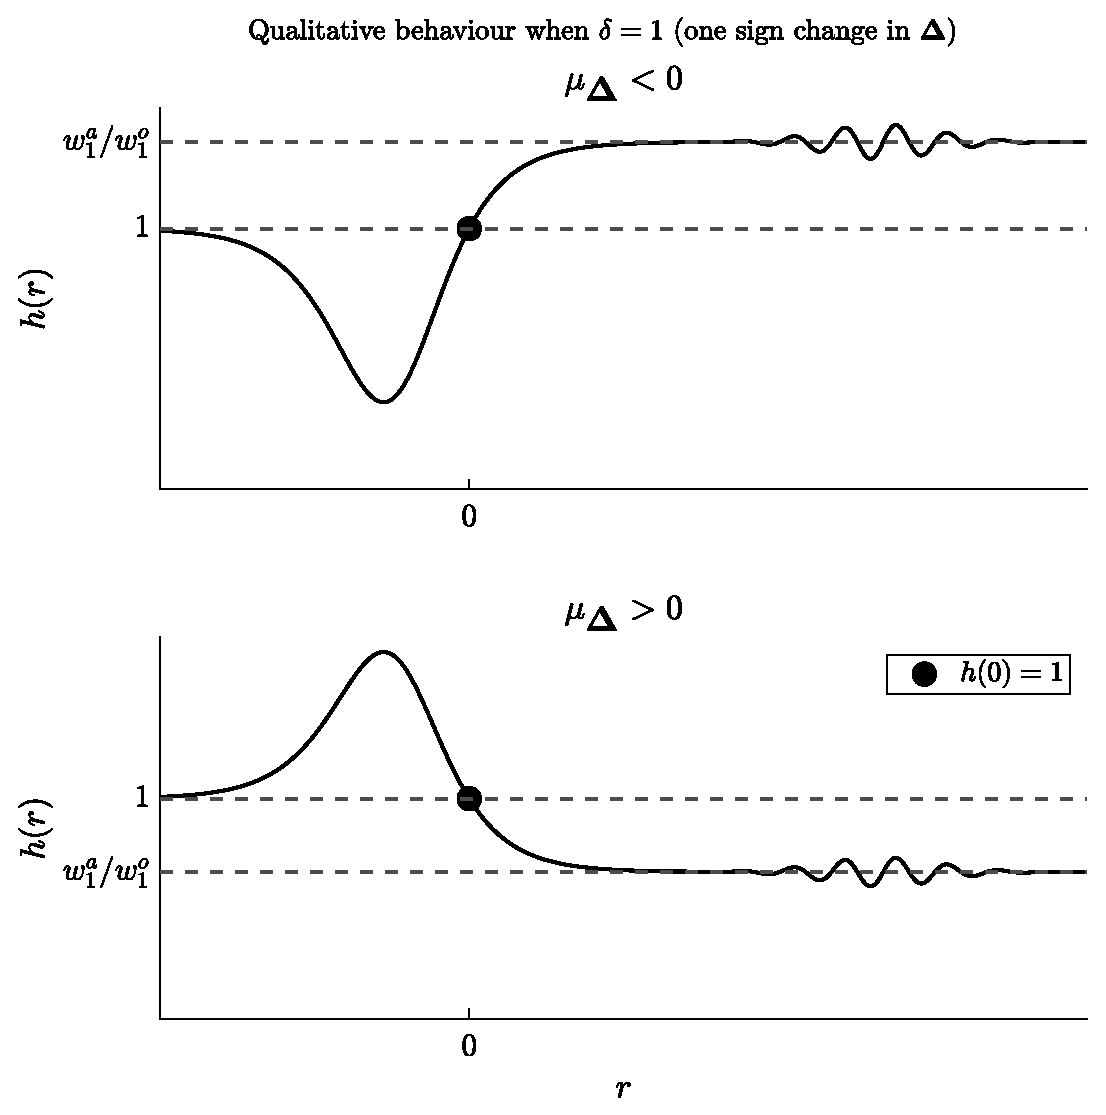
\includegraphics[width=\linewidth]{Figures/Delta_Eq_1_Schematic.eps}
\captionof{figure}{This figure summarises the only two cases when $\delta=1$. When the curve is greater than 1, this illustrates an over-estimate. Conversely, when the curve is less than 1, this illustrates an under-estimate.}
\label{fig:Delta_Eq_1}
\end{minipage}

Figure \ref{fig:Delta_Eq_1_Area} computationally verifies the theory predicted mathematically in Figure \ref{fig:Delta_Eq_1}. We chose a selection of $\boldsymbol{\Delta}$s that varied linearly in $\mu_{\boldsymbol{\Delta}}$ (from 1 to -1), whilst maintaining the condition that $\mu_{\boldsymbol{\Delta}}\cdot \Delta_1 <0$. For details on how we generated these $\boldsymbol{\Delta}$s, see section X. (\textbf{see code section on Notability for details}). The reader should note that there is no significance to the horizontal band on the right hand side sub-figure of Figure \ref{fig:Delta_Eq_1_Area}. This is because this corresponds to $w^a = w^o$, and so there is no difference in inference. Of course, we could have chosen a different family of $\boldsymbol{\Delta}$ such that the mean was 0 but the corresponding $\boldsymbol{\Delta}$ was not $\boldsymbol{0}$. The important features that Figure \ref{fig:Delta_Eq_1_Area} picks up on are:

\begin{enumerate}
    \item The convergence of $h(r)$ to 1 as $r \rightarrow  \infty$ (The difference in inferences seems to tend to zero as $R_t \rightarrow  0^+$.), see right sub-plot.
    \item $h(r)=1$ when $r=0$ ($R_t=1$), see right sub-plot.
    \item The over-estimating of $R_t$ when $\mu_{\boldsymbol{\Delta}}<0$ and under-estimating of $R_t$ when $\mu_{\boldsymbol{\Delta}}>0$
    \end{enumerate}
   
\begin{figure*}
  \centering
  
    \begin{minipage}{\linewidth}
    \centering
    \begin{tikzpicture}[boximg]
      \node (img1) {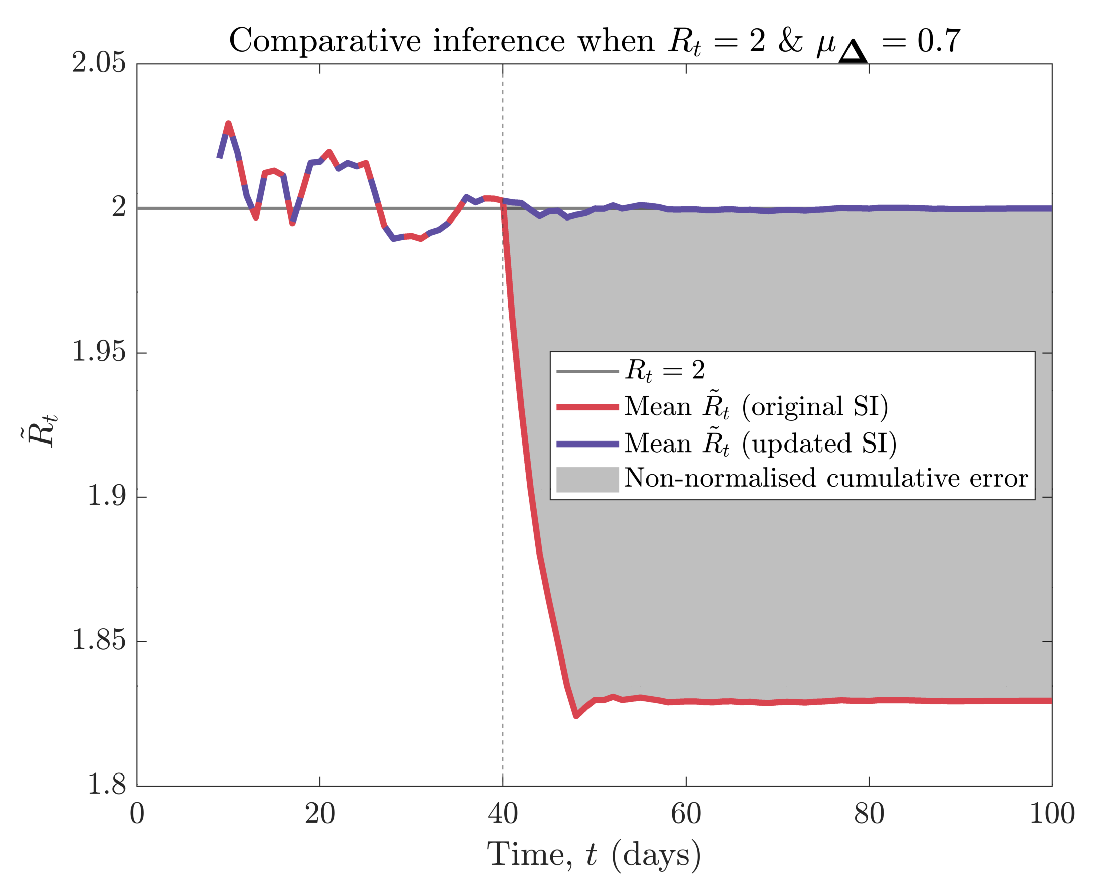
\includegraphics[width=0.3\linewidth]{Figures/Report_Example_1_delta_eq_1.eps}};
      \draw (img1.south west) rectangle (img1.north east);
    \end{tikzpicture}\hfill
  \end{minipage}\\[0.5\baselineskip]
  \begin{minipage}{\linewidth}
    \begin{tikzpicture}[boximg]
      \node[anchor=south west] (img) {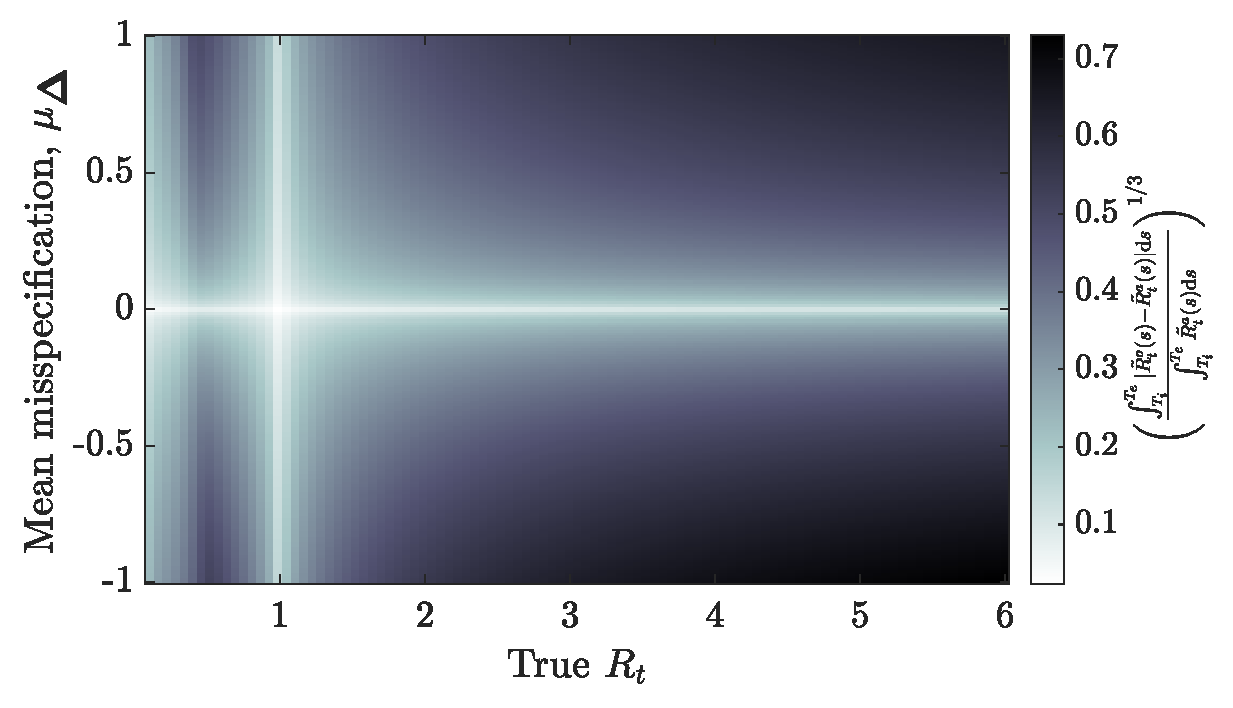
\includegraphics[width=\linewidth]{Figures/Area_R_t_delta_eq_1.eps}};
      \begin{scope}[x=(img.south east),y=(img.north west)]
        \node[draw,minimum height=.163cm,minimum width=0.163cm] (B1) at (0.157,0.8505) {}; %Small red-boxes on main figure:Size in [,] and position in (,)
        \node[draw,minimum height=0.163cm,minimum width=0.163cm] (B3) at (0.325,0.303) {};
      \end{scope}
    \end{tikzpicture}
  \end{minipage}\\[0.5\baselineskip]
  \begin{minipage}{\linewidth}
  \centering
    \begin{tikzpicture}[boximg]
      \node (img3) {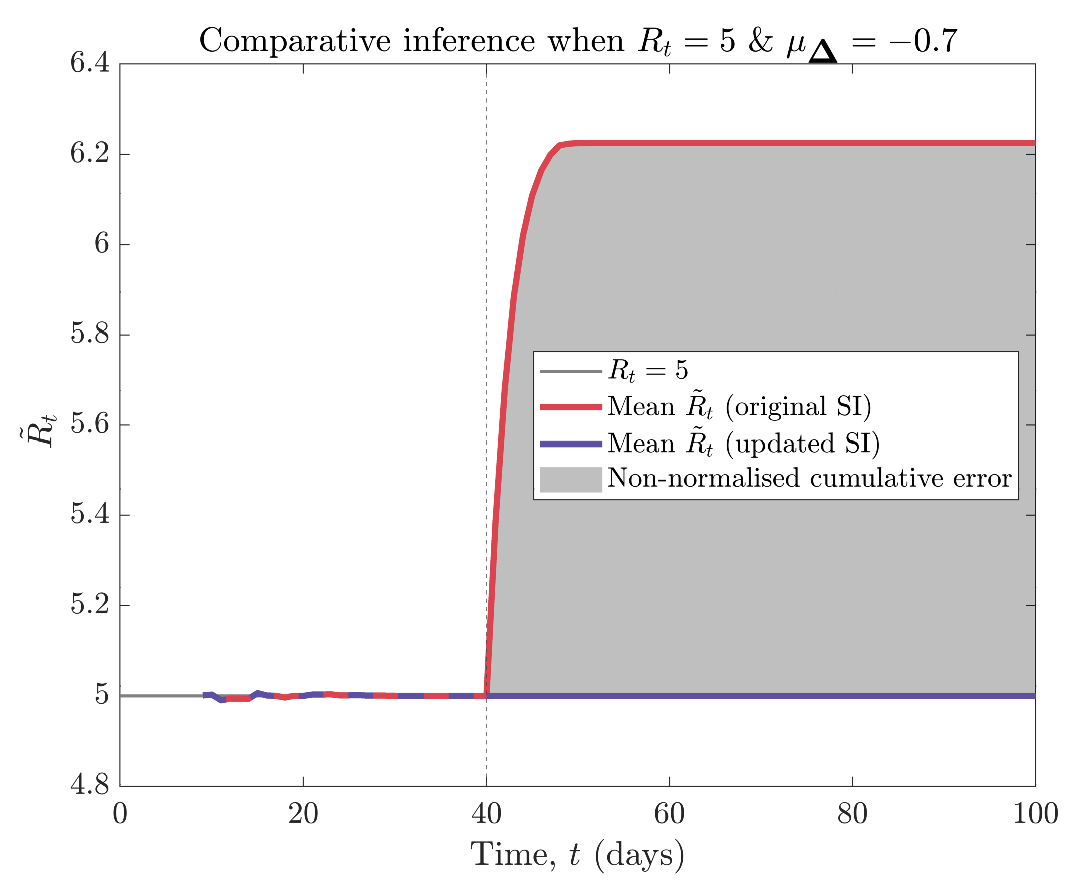
\includegraphics[width=0.3\linewidth]{Figures/Report_Example_2_delta_eq_1.eps}};
      \draw (img3.south west) rectangle (img3.north east);
    \end{tikzpicture}\hfill
  \end{minipage}
  \begin{tikzpicture}[overlay,boximg]
    \draw (B1) -- (img1);
    \draw (B3) -- (img3);
  \end{tikzpicture}
  \caption{The National Gallery of Canada}
\end{figure*}

\begin{figure*}
  \centering
  
    \begin{minipage}{\linewidth}
    \centering
    \begin{tikzpicture}[boximg]
      \node (img1) {\includegraphics[width=0.3\linewidth]{example-image-10x16}};
      \draw (img1.south west) rectangle (img1.north east);
    \end{tikzpicture}\hfill
    \begin{tikzpicture}[boximg]
      \node (img2) {\includegraphics[width=0.3\linewidth]{example-image-10x16}};
      \draw (img2.south west) rectangle (img2.north east);
    \end{tikzpicture}\hfill
  \end{minipage}\\[0.5\baselineskip]
  \begin{minipage}{\linewidth}
    \begin{tikzpicture}[boximg]
      \node[anchor=south west] (img) {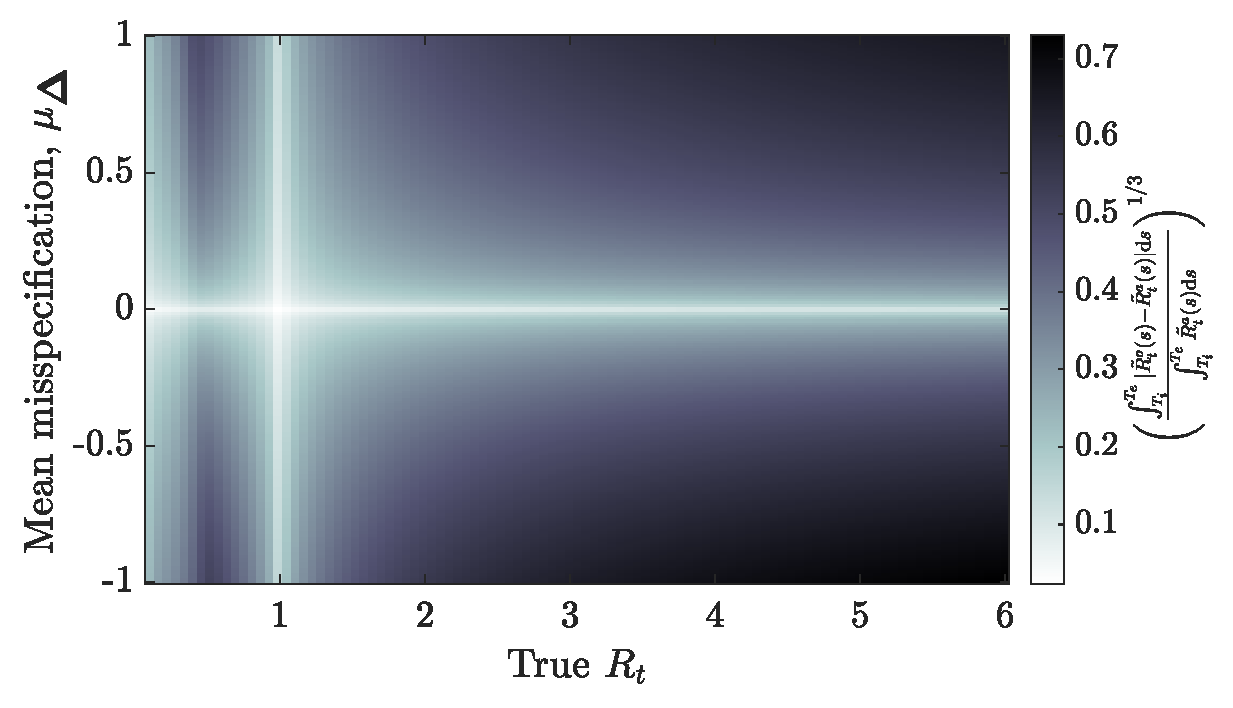
\includegraphics[width=\linewidth]{Figures/Area_R_t_delta_eq_1.eps}};
      \begin{scope}[x=(img.south east),y=(img.north west)]
        \node[draw,minimum height=.6cm,minimum width=1.00cm] (B1) at (0.5,0.60) {}; %Small red-boxes on main figure:Size in [,] and position in (,)
        \node[draw,minimum height=0.8cm,minimum width=0.50cm] (B2) at (0.7,0.25) {};
        \node[draw,minimum height=0.8cm,minimum width=0.50cm] (B3) at (0.1,0.25) {};
      \end{scope}
    \end{tikzpicture}
    \caption{}
  \end{minipage}\\[0.5\baselineskip]
  \begin{minipage}{\linewidth}
    \begin{tikzpicture}[boximg]
      \node (img3) {\includegraphics[width=0.3\linewidth]{example-image-10x16}};
      \draw (img3.south west) rectangle (img3.north east);
    \end{tikzpicture}\hfill
  \end{minipage}
  \begin{tikzpicture}[overlay,boximg]
    \draw (B1) -- (img1);
    \draw (B2) -- (img2);
    \draw (B3) -- (img3);
  \end{tikzpicture}
  \caption{The National Gallery of Canada}
\end{figure*}

The diagram shows that if we are able to prove that in the real world, $\delta=1$, we can make concrete assertions about whether we are over/under-estimating $R_t$.\\

Unfortunately, the consequences when $\delta=2$ is marginally more mathematically complex which means the real-world consequences for $R_t$ estimation when $\delta=2$ are difficult to summarise. In short, it is no longer so obvious whether or not we have over/under-estimated $R_t$. As opposed to when $\delta=1$, there are now 4 cases (combinations of $\mu_{\boldsymbol{\Delta}} \lessgtr 0$ and $\Delta_1 \lessgtr 0$) to consider for the shape of $h(r)$ (since we can no longer eliminate two of the cases as we could previously). Rather than summarising what this means for the over/under-estimates, we refer the reader to Figure \ref{fig:Delta_Eq_2}.

\begin{figure*}
\centering
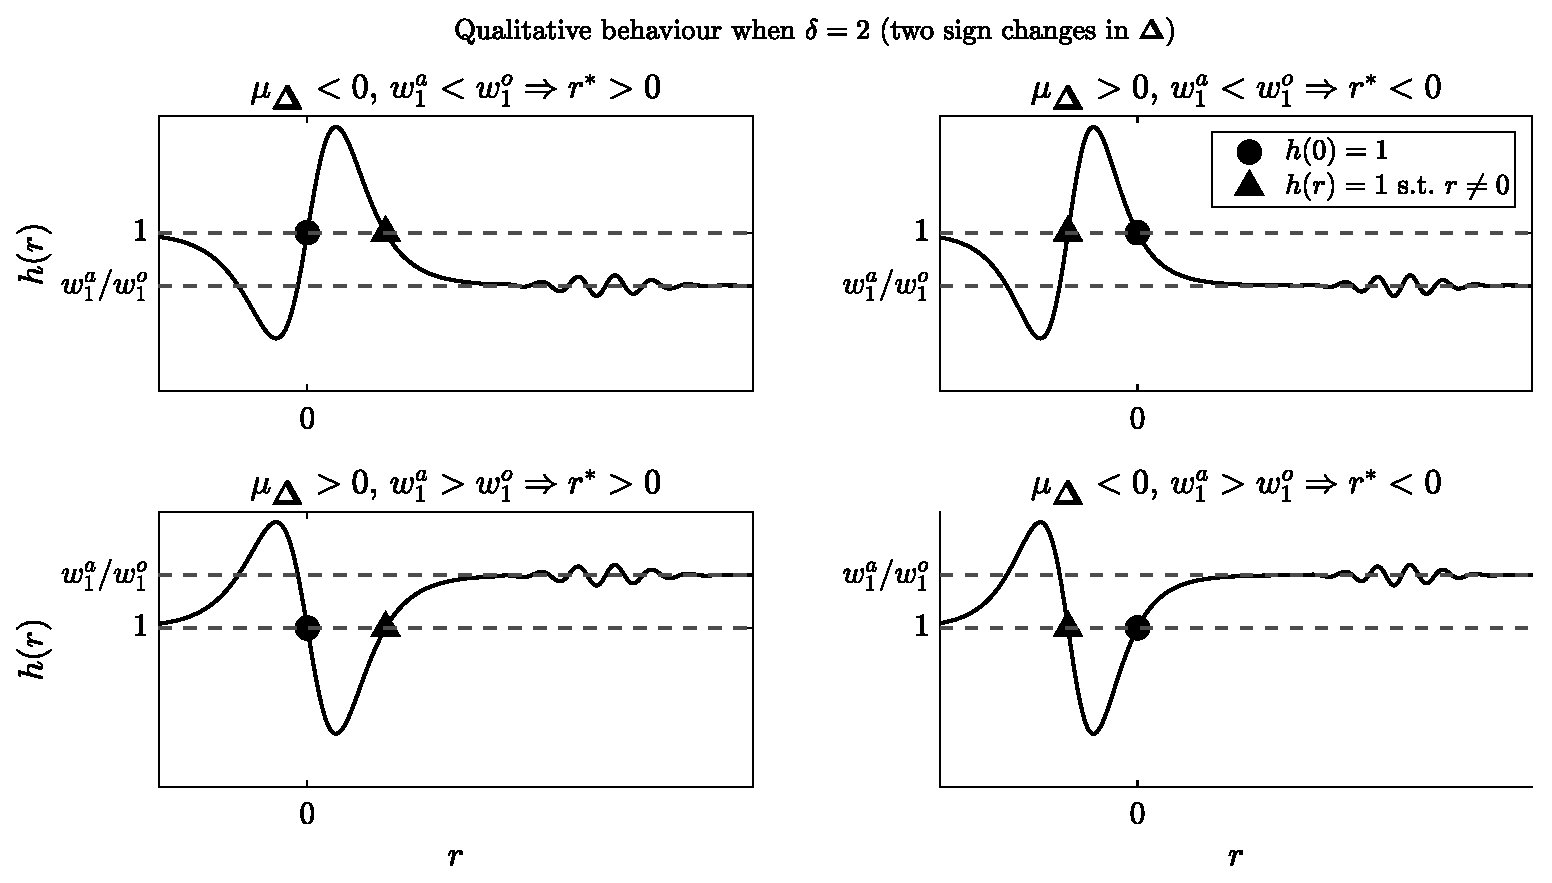
\includegraphics[width=\linewidth]{Figures/Delta_Eq_2_Schematic.eps}
\captionof{figure}{Unlike the case when $\delta=1$, there is no implication for $\mu_{\boldsymbol{\Delta}}$ when $\Delta_1$ takes a particular sign (or vice versa). This implies that there are 4 cases to consider instead of 2. Similarly, the curve being greater or less than 1 indicates an over/under-estimate respectively.}
\label{fig:Delta_Eq_2}
\end{figure*}



\subsubsection{Shape of $h(c)$ local to $c=0$}
We recall that 
\begin{align*}
L'(x) &= -\sum_{i=1}^{N}e^{-ix}iw_i \\
\implies L''(x) &= \sum_{i=1}^{N}e^{-ix}i^2w_i
\end{align*}
We can deduce that $L'(0) = -\mathbb{E}[\boldsymbol{w}]$ and $L''(0) = \mathrm{Var}[\boldsymbol{w}]+\mathbb{E}[\boldsymbol{w}]^2$.\\
The quotient rule and the repeated quotient rule say that
\begin{align*}
&\text{if }
    h(x)&&= \frac{f(x)}{g(x)} \text{,}\\
    &\text{then }
    h'(x)&&= \frac{f'(x)g(x) - f(x)g'(x)}{g^2(x)}\\
    &\text{and }
    h''(x)&&= \frac{f''(x)g(x)-f(x)g''(x)}{g^4(x)}
\end{align*}

As will become clear, we only need to be concerned about the \textit{sign} of the first and second derivative of $h$ at $c=0$. Since both $g^2(x)>0 \forall x$ and $g^4(x)>0 \forall x$ we only need to consider the numerator.

\begin{align*}
\mathrm{sgn} \{ h'(c)\} &= \mathrm{sgn} \{\Large[qte^{ct}L_a(c) +qe^{ct}L_a'(c)\Large] \cdot \Large[ p+q e^ct L_o(c) \Large] \\ 
&- \Large[qte^{ct}L_o(c) +qe^{ct}L_o'(c)\Large] \cdot \Large[ p+q e^ct L_a(c) \Large] \}\\
\implies \mathrm{sgn} \{ h'(0)\}&= \mathrm{sgn} \{qL_a'(0)(p+q)-qL_o(o)(p+q) \}\\
&= \mathrm{sgn} \{ q(p+q)\Large( L_a'(0) - L_o'(0)\Large) \}\\
&= \mathrm{sgn} \{ q(p+q)(\mu_o-\mu_a) \}
\end{align*}

\begin{equation*}
\begin{split}
\mathrm{sgn} \{ h''(c)\} &= \mathrm{sgn} \{\Large[ qe^{ct}L_a(c)+qt^2e^{ct}L_a(c)\\
&+ qte^{ct}L_a'(c)+qe^{ct}L_a''(c) \Large] \cdot \Large[(p+qe^{ct}L_o(c) \Large]\\ 
&- \Large[ qe^{ct}L_o(c)+qt^2e^{ct}L_o(c)\\
&+ qte^{ct}L_o'(c)+qe^{ct}L_o''(c) \Large] \cdot \Large[p+qe^{ct}L_a(c) \Large] \} \\
\implies \mathrm{sgn} \{ h''(0)\}&= \mathrm{sgn} \{q(p+q)\{ \Large(1+ \mu_a^2 +\sigma_a^2 \Large) - \Large( 1+ \mu_o^2 +\sigma_o^2 \Large) \}\\
&= \mathrm{sgn} \{q(p+q)(\mu^2_a-\mu_o^2 + \sigma_a^2 -\sigma_o^2) \}
\end{split}
\end{equation*}

Now we are equipped with both the sign of $h'(0)$ and $h''(0)$, as well as how many zeros $h(c)$ has. We also know the behaviour of $h(c)$ as $c \rightarrow \pm \infty$.\\
When it comes to sketching $h(c)$ (which is critical to determining how divergent $\tilde{R}_t^o$ is to $\tilde{R}_t^a$), it turns out that only $\delta$ and $\mu_d$ ($\mu_a- \mu_o$) are the important factors. There is of course the unusual case where $\mu_d=0$, in which case $\mathrm{Var}(\Delta)$ becomes important once again.

For example, if 
\begin{enumerate}
    \item $\boldsymbol{\Delta}$ has one sign change
    \item $\mu_a =\mu_o$
    \item $\sigma_a > \sigma_o$,
\end{enumerate}
then $h(c)>1 \forall c \ne 0$, i.e. we will always over-estimate the true $R_t$, unless $R_t = 1$ ($c=0$).\\

-----------------------------------


Formal verification of these hypotheses should be mathematical in nature, and we hope that the Appendix provides the reader with a robust reasoning as to why H\ref{hyp:first}, H\ref{hyp:thirda}-\ref{hyp:thirdf}, and H\ref{hyp:second} hold. This section can only serve as a computational verification of these results\footnote{It is important to note again that all of these hypotheses make reference to $h$ as a function of $r$ (\textit{epidemic growth rate}), where as the Methods section outlines inference methods for $R_t$ (\textit{time-dependant reproduction number}). It is sufficient for the reader to note that this report implements the relationship between $r$ and $R_t$ \cite{Wallinga-Lipsitch}, the modification of which are outlined in Appendix.}. All three hypotheses are tested using large simulations across a range of $\boldsymbol{\Delta}$s, which vary in $\mu_{\boldsymbol{\Delta}}$ and $w$ in accordance with the assumptions in the hypotheses. Where stochasticity plays a significant role, we either repeat simulations, or remove stochasticity all-together, to investigate the mean behaviour. We therefore stress that this section can only prove a hypothesis to be incorrect, as opposed to anything else.\\



\subsection{Numerical Results}

\begin{minipage}{0.95\linewidth}
\centering
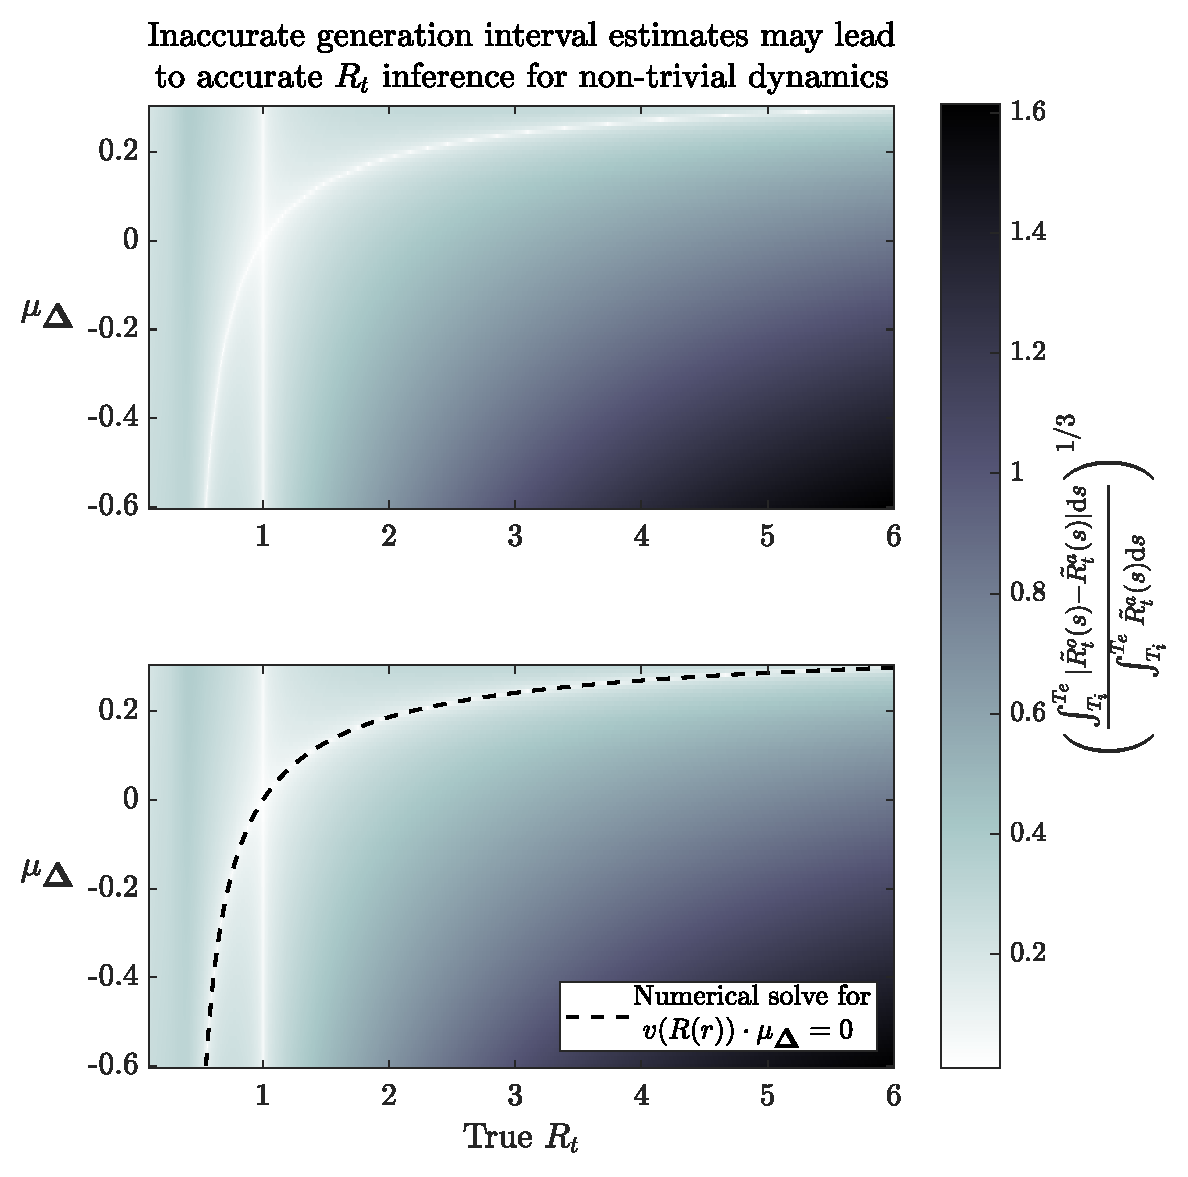
\includegraphics[width=\linewidth]{Figures/Significant_Finding_1.eps}
\captionof{figure}{}
\label{fig:Significant_Finding}
\end{minipage}

Plots of simulations.\\

Time varying $R_t$ plots.\\

\textbf{Discussion} 9\\

Summarise results from results section. There is a question about how to do this. Perhaps through a table.\\

Discussion of the fact that the key characteristics are unknown since we do not know what the true serial interval is. It may be that two out of three of the important quantities are known- can we still quantify the over/under-estimate?\\

Discussion of how we may be able to have guesses about these quantities by how data is collected to generate serial intervals.\\

$\delta$: Why we only considered $\delta=1$, $\delta=2$, but should more be considered? What about multi-modal GIs? Is it ever possible to know what $\delta$ is? \\

$\mu_{\Delta}$: When might we know what the sign of this is?\\

$w_1^o/w_1^a -1$: When might we know what the sign of this is?\\

Figure that Robin suggested (relating true $R_t$ to inferred $R_t$) and discussion of significance\\

Why $\sigma$ is unimportant.\\

Extensions: Discussion of whether a continuously time varying SI will give results that are explained by this report? Can we use real data to simulate this? Would this have affected interventions?\\


 

 
 \subsection{Standard Method}
 
 Cori et al. \cite{Cori-Ferguson}, Thompson et al. \cite{Thompson-Stockwin} have developed Bayesian inference techniques to estimate the \textit{instantaneous} reproduction number. This method will form the basis for much of our analysis. \textbf{Describe method in full!}
 
 Figure \ref{fig:Maryland} shows $R_t$ inference during the Influenza outbreak in Maryland, USA in 1918. Figure \ref{fig:Maryland} illustrates both the $R_t$ inference (and associated confidence intervals) as well as the incidence data. We include both here to demonstrate how the $R_t$ inference relates to the data but for the rest of this report, we will not include both since we will be plotting multiple inferences. In principle, we can align the time axis with actual dates and consequently evaluate how the statutory measures affected the reproduction rate. Reports from 1918 (influenzaarchive.org/cities/city-baltimore.html#) make this kind of analysis possible. Recent examples include \textbf{Find paper where they work out what interventions do to R}, where they were able to determine the effectiveness of selected NPIs in driving down the $R$ number.\\
 
 It is worth noting an important feature of this graph, which should be explained before we begin our own analysis. The confidence interval tends to be narrower when there are a large number of cases, which is illustrated quite clearly in figure \ref{fig:Maryland}. For much of our analysis, we will generate data synthetically- show figure and explain!
 
 \textbf{Put in another figure that narrows the confidence interval and explain feature}
 
 \begin{minipage}{\linewidth}
\centering
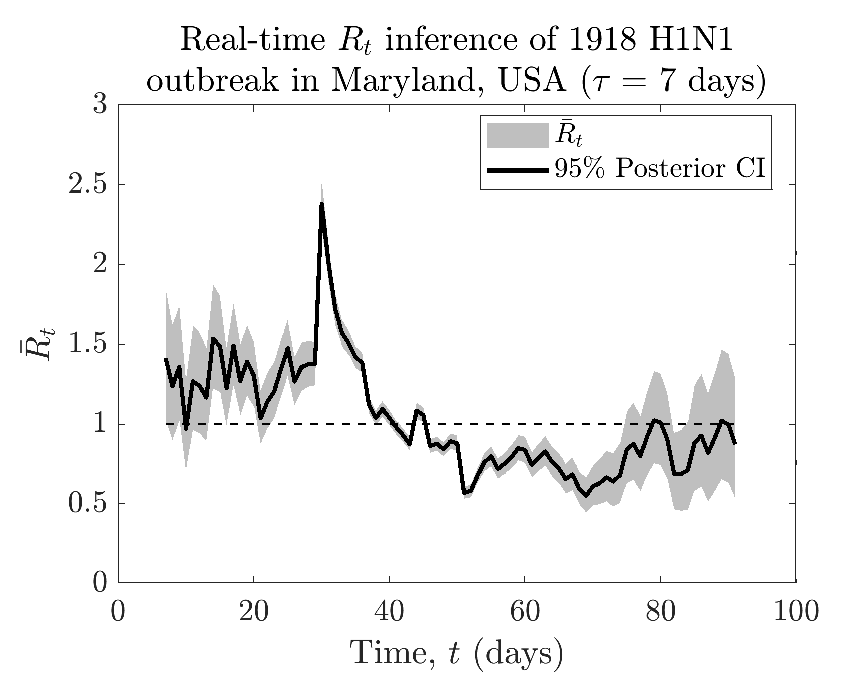
\includegraphics[width=\linewidth]{Figures/H1N1_Maryland_1918_Estimate_CI_Zoom.eps}
\captionof{figure}{}
\label{fig:Maryland}
\end{minipage}
 
%  \subsection{\textit{Hybrid} serial intervals}
 
%  A \textit{hybrid} SI, $\tilde{w}_i^j$ is a term we use to describe the transitory state of a serial interval when new information is provided to update the SI. More specifically, the hybrid $SI$ is a sequence of PMFs that appropriately transition from the `original' to the `actual' serial interval. Note that these hybrid SIs do not account for the fact that the population may be less adherent, which would require additional complexity. However, even with $100\%$ adherence, we should model some transitional SIs. The update procedure requires knowledge about \textit{when} the SI switched from the `original' to the `actual' SI and in some cases the hybrid SI may be irrelevant. For example, if the control measure corresponding to the SI switch occurred six months prior to the new SI becoming available, then there will be no hybrid SI since we would simply be correcting the SI. However, hybrid SIs do become relevant when we are have updated SI estimates close to the control measure date \footnote{In reality, these estimates require more time to infer, although reasonable guesses may be made particularly if the control measure dictates behaviour change such as quarantining.}. This is because we will be using incidence data either side of the control measure so the model predicts that some of the infection will still be contributed from transmission prior to the control measure. We would also expect that the probability of someone infecting someone else after the intervention (but according to the old SI) will reduce (because the probability is in some way decreased when the individual hears about new control measures). We believe this is accounted for by the normalisation procedure.\\
%  It is worth noting that there is at least one way to model the transitory evolution of the hybrid SIs. Here, we formally describe our approach with all terms defined, assuming instantaneous calculation of the SI on the day of control measures being introduced (the approach is easily modified for non instantaneous calculation).
%  \begin{indenteddesc}
%  \item[$T$] is the time of the control measure being introduced (assuming 100)
%  \item[$\tilde{w}_k^{T+k}$] is the serial interval used at time $T+k$ at the $k$th index, i.e. the probability of subsequent symptoms appearing $k$ days apart at time $T+k$.
%  \end{indenteddesc}
 
%  Here, we consider an update that is truncated, i.e. $N_a<N_o$ to illustrate the potential complexity of a different domain over the SI. Note that we also focus on time after an intervention.
 
%  \begin{equation}
%   \tilde{w}_k(t+k) =
%     \begin{cases}
%       0 & \text{if } 2k>L\\
%       \alpha w^a_k  & \text{if } k \leq N_a\\
%       \alpha w^o_k & \text{if }k \in [N_a+1, N_o-k] ^*
%     \end{cases}       
% \end{equation}
%  $^*$ Note that this set will be empty if $\exists k$ s.t. $N_a> N_o-k-1$.\\
 
%  In practice, these hybrid SIs factor in two concepts:
 
%  \begin{enumerate}
%      \item The contribution from the actual serial interval becomes increasingly relevant through time,
%      \item The contribution from the original serial interval becomes decreasingly relevant through time.
%  \end{enumerate}
% This is demonstrated in the following \ref{fig:Hybrid_Progression}:



% One obvious problem with the implementation of hybrid SIs is that, even if the data were available, it would take several weeks to construct the `actual' SI. This means the assumption that we can have this SI instantly is naïve at best. However, it is worth considering if there are ways to estimate what the actual SI may be. There is potential for this when the control measure has a fairly predictable impact on behaviour, e.g. quarantining measures are likely to truncate the SI.\label{sect:Method}
 

  
\subsection{Synthetic Data}

As discussed in section \ref{sect:Results}, there is a multitude of ways in which we can analyse the effect of improved serial interval distributions. We divide our analysis into multiple subsections, listed in the following table:

Throughout this section, the data has been generated synthetically. We do this by first pre-determining an $R_t$ time series and a `true' serial interval, $w_s^t$. We compute incidence data at each day by assuming that incidence behaves akin to a branching process with a Poisson distribution and rate $R_t\Lambda_t (w_s)$ assume a large population size. We then implement the method described in \ref{sect:Method} and we monitor the affect of a time-varying serial interval. Note that, if we wanted our model to be realistic, there would be some further effect on $R_t$ if for instance the mean SI decreased. We attempt to model this case in section \textbf{X}.
  
\subsubsection{Constant $R_t$}\label{sect:Constant_R}

The following figures summarise the behaviour of the effect of using/not using updated SIs. We assume, when implementing updated SIs, that perfect information is available at the moment the true SI changes.\\
There are many ways in which a serial interval changes through time. This is normally due to control measures being put in place, the public being more aware of the disease or becoming weary of adhering to control measures. We can infer reasonable assumptions about how the SI distribution changes.\\
In this sub-section, we create a mass function, that is the discrete analogue of a $N(8, 2)$ distribution, that has been truncated up to 15 days. The data is generated using a true $R_t$ equal to 2.
\begin{minipage}{\linewidth}
\centering
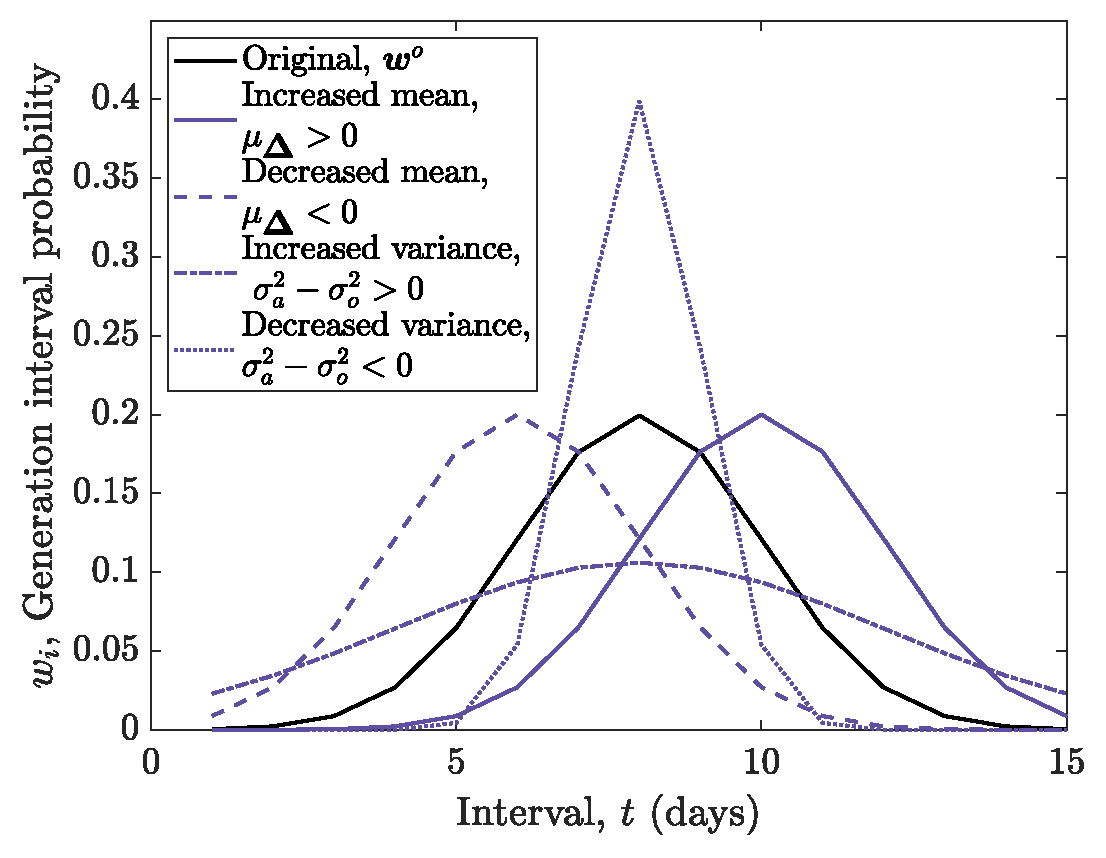
\includegraphics[width=\linewidth]{Figures/Report_Constant_R_Disc_Serial_0.eps}
\captionof{figure}{}
\label{fig:Constant_R_Disc_Serial_0}
\end{minipage}  
  
\begin{minipage}{\linewidth}
\centering
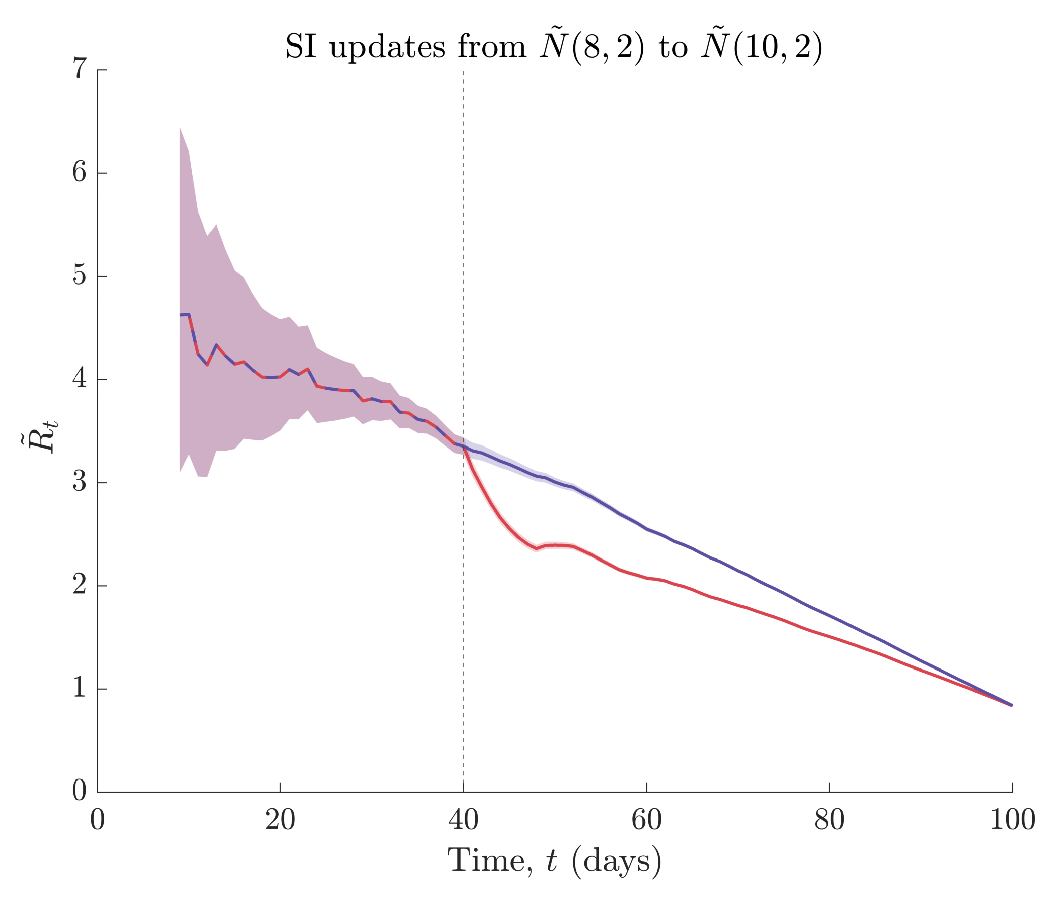
\includegraphics[width=\linewidth]{Figures/Report_Constant_R_Disc_Serial_1.eps}
\captionof{figure}{The horizontal, grey line illustrates how good the method is at back-inferring the true $R_t (=2)$. The vertical horizontal line illustrates when the SI changes.}
\label{fig:Constant_R_Disc_Serial_1}
\end{minipage}

\begin{minipage}{\linewidth}
\centering
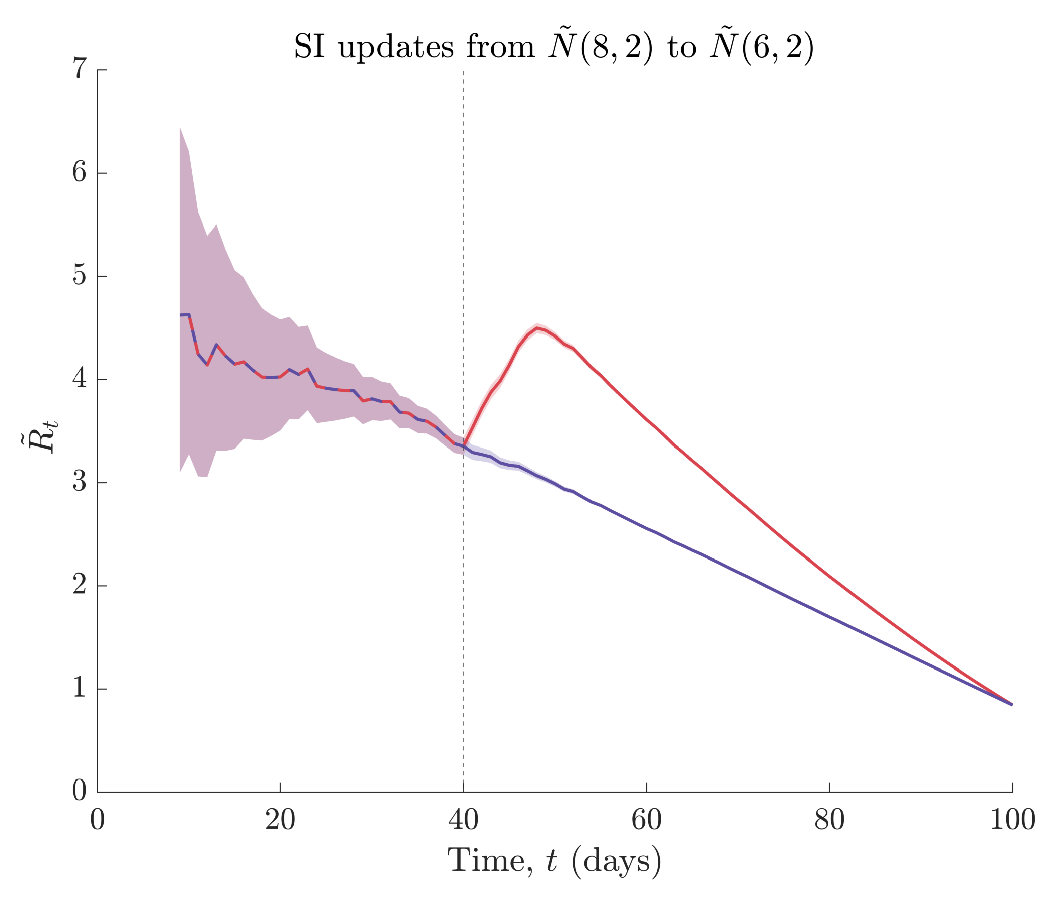
\includegraphics[width=\linewidth]{Figures/Report_Constant_R_Disc_Serial_2.eps}
\captionof{figure}{}
\label{fig:Constant_R_Disc_Serial_2}
\end{minipage}

\begin{minipage}{\linewidth}
\centering
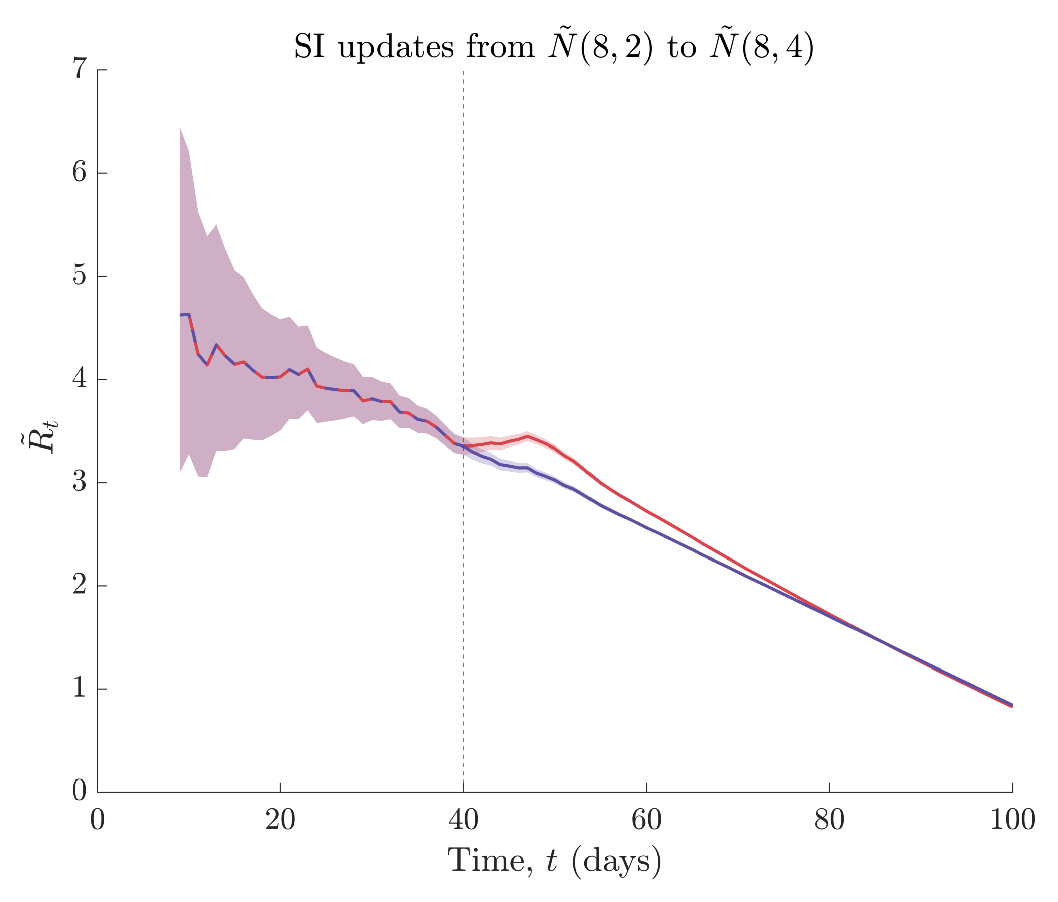
\includegraphics[width=\linewidth]{Figures/Report_Constant_R_Disc_Serial_3.eps}
\captionof{figure}{}
\label{fig:Constant_R_Disc_Serial_3}
\end{minipage}

\begin{minipage}{\linewidth}
\centering
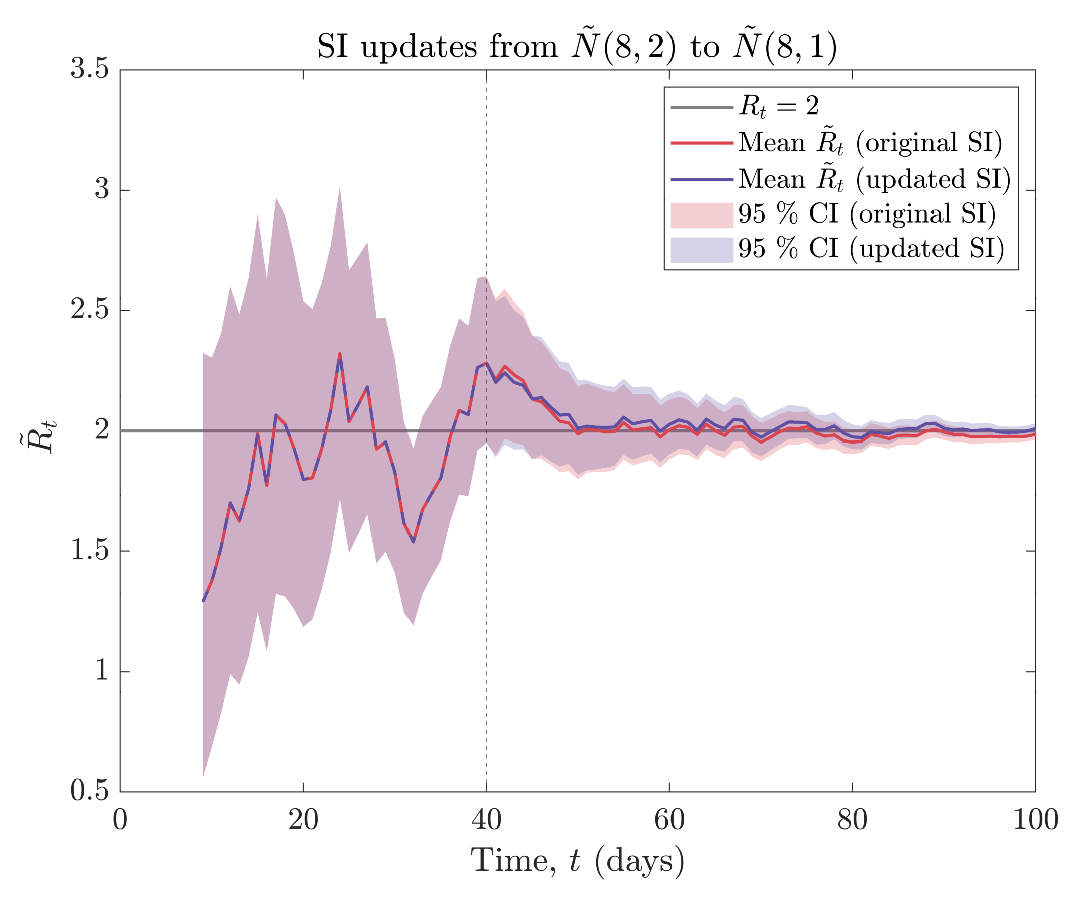
\includegraphics[width=\linewidth]{Figures/Report_Constant_R_Disc_Serial_4.eps}
\captionof{figure}{}
\label{fig:Constant_R_Disc_Serial_4}
\end{minipage}

What we can conclude about figures \ref{fig:Constant_R_Disc_Serial_1} and \ref{fig:Constant_R_Disc_Serial_2} is that ``if the recorded mean SI is over-estimated, then $R_t$ will be over-estimated.'' And likewise ``if the recorded mean SI is under-estimated, then $R_t$ will be under-estimated.''\\
It is not obvious from figures \ref{fig:Constant_R_Disc_Serial_3} and \ref{fig:Constant_R_Disc_Serial_4} to summarise how over/under-estimates of the SI variance affect $R_t$ inference without making reference to figure \ref{fig:Constant_R_Disc_Serial_Variance_Analysis}. This shows that ``an over-estimate of the variance leads to an under-estimate of $R_t$'' whilst ``an over-estimate of the variance leads to an under-estimate of $R_t$''.

\textbf{Discuss that we expect the opposite results when $R<1$.}

\begin{minipage}{\linewidth}
\centering
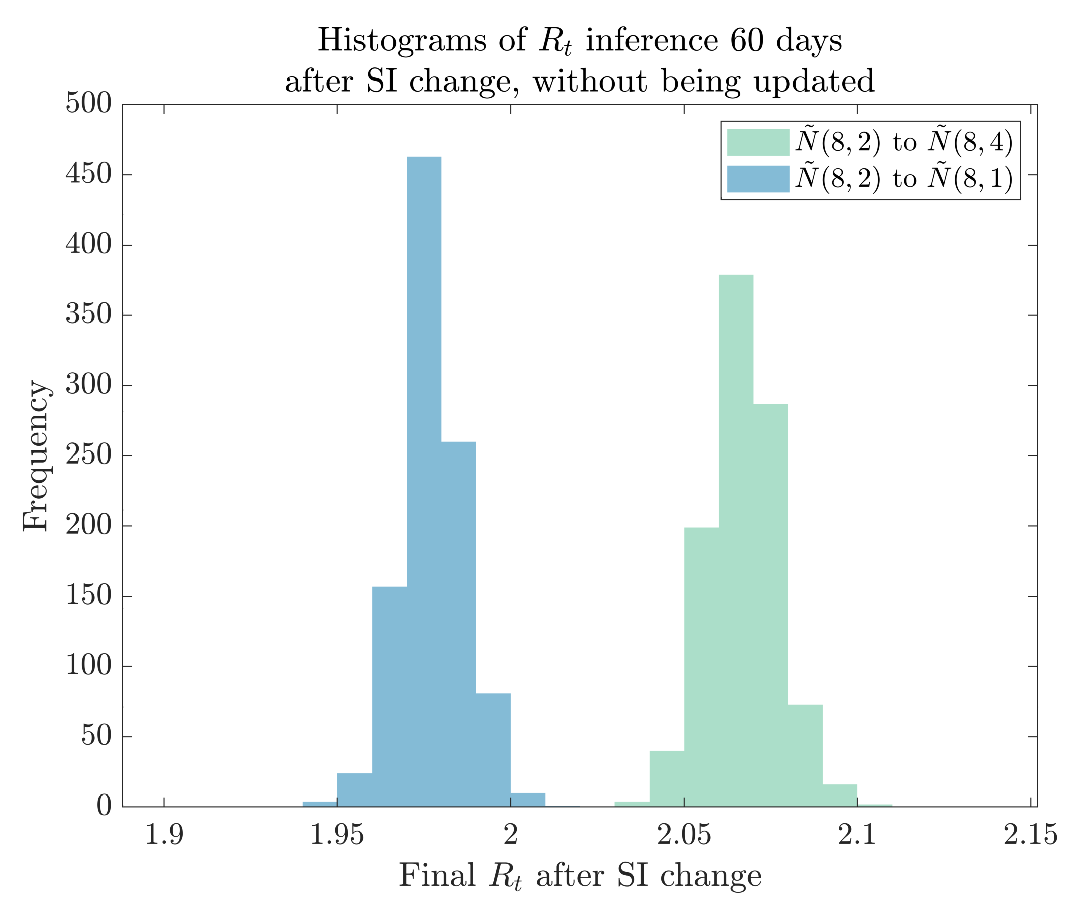
\includegraphics[width=\linewidth]{Figures/Report_Constant_R_Disc_Serial_Variance_Analysis.eps}
\captionof{figure}{1000 simulations were ran in an identical manner to the time-series in figures \ref{fig:Constant_R_Disc_Serial_3} and \ref{fig:Constant_R_Disc_Serial_4}. $\tilde{R}_100$ was recorded for each simulation and these are the values that make up the histogram.}
\label{fig:Constant_R_Disc_Serial_Variance_Analysis}
\end{minipage}
  
\subsubsection{$R_t$ varying linearly with time}\label{sect::Linear_R}

The previous sub-section motivates this section of study. If poor SI estimates leads to poor estimates of the effective $R$ number when the dynamics are simple, what happens when we introduce more complexity? The obvious increment in complexity is to no longer generate data using a constant $R_t$, and instead use a variable $R_t$ that is linear in time. It is also worth considering how inference will differ if $R_t$ is increasing or decreasing.\\

Prior to viewing the results, it is important to study $R_t$ inference when there is no change in serial interval. The top-left sub-plot in figure \ref{fig:Vary_Lin_Decrease_R_Disc_Serial_All} highlights the distinction between the true $R_t$ and the inferred $\tilde{R}_t$, which was present when the true $R_t$ was constant in time.

% \begin{minipage}{\linewidth}
% \centering
% 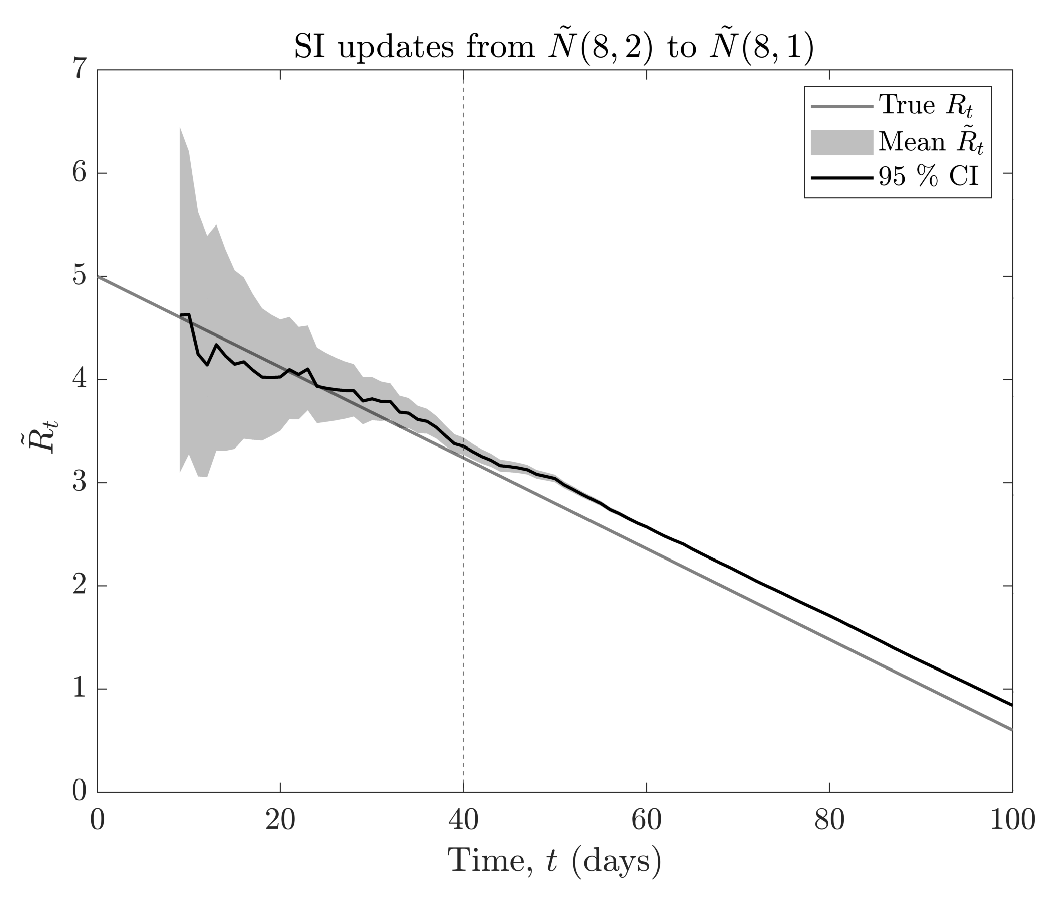
\includegraphics[width=\linewidth]{Figures/Report_Vary_Lin_Decrease_R_Disc_Serial_o.eps}
% \captionof{figure}{}
% \label{fig:Vary_Lin_Decrease_R_Disc_Serial_o}
% \end{minipage}

% \begin{minipage}{\linewidth}
% \centering
% 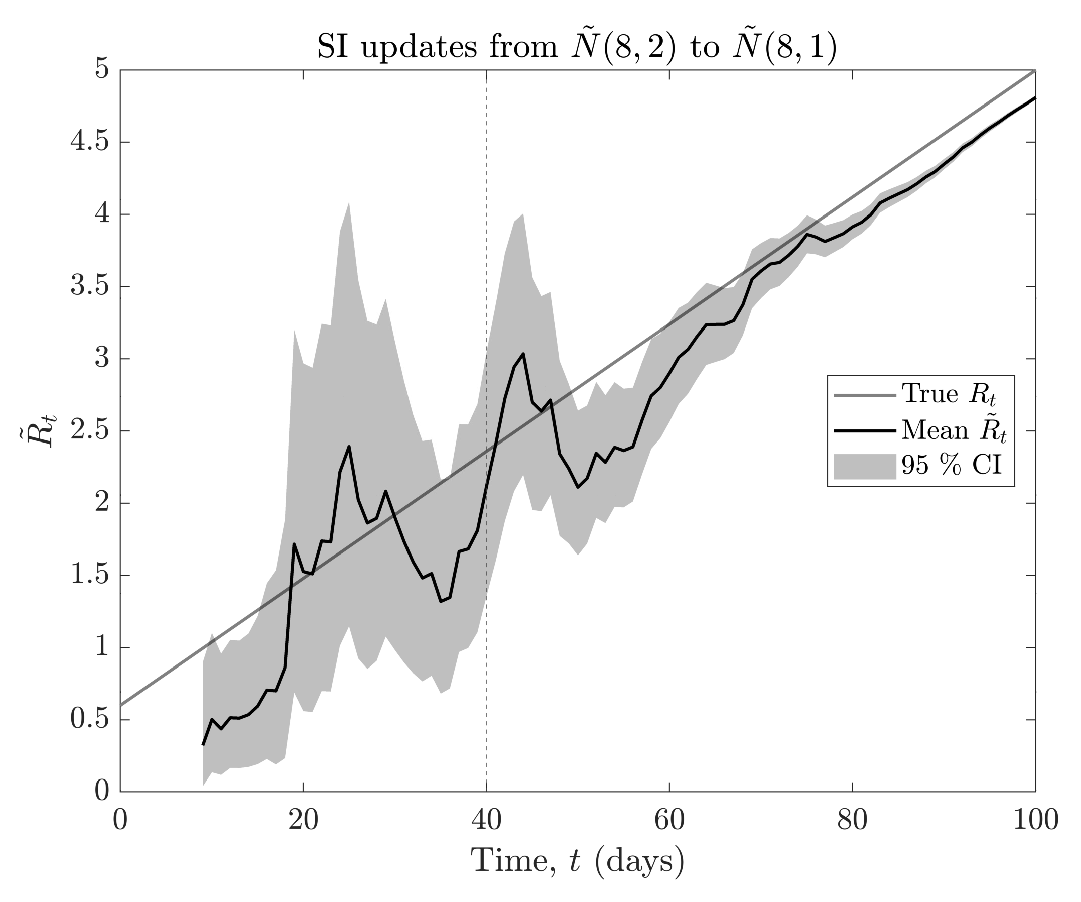
\includegraphics[width=\linewidth]{Figures/Report_Vary_Lin_Increase_R_Disc_Serial_o.eps}
% \captionof{figure}{}
% \label{fig:Vary_Lin_Increase_R_Disc_Serial_o}
% \end{minipage}

This deviation is consistent after $\sim 50$ days and equates to $\approx 5.5$ day lag, i.e.  $$\tilde{R}_t \approx R_{t-5.5}.$$ This is a result of the modelling simplification that $R_t$ is constant during inside the $[t-\tau +1, t]$ time window. We note that this issue was raised in the Section \ref{sect:Methodology} and was necessary in order to use Bayes' Theorem. As discussed, we can reduce this disparity by reducing $\tau$, with the side-effect of making $R_t$ inference more sensitive to randomness in incidence data.\\
In this case, $\tau=8$, and so we will treat Figure \ref{fig:Vary_Lin_Decrease_R_Disc_Serial_o} as the typical best case scenario. It follows that the a good inference for a linearly changing $R_t$ will pick up the rate at which $R_t$ is increasing, although we expect there will always be some offset due to the nature of instantaneous reproduction numbers, i.e. if $R_t = at +b$, $\tilde{R}_{\text{best}} = at+c$ \\

The remaining sub-plots in figure \ref{fig:Vary_Lin_Decrease_R_Disc_Serial_All} summarise the discrepancies in estimating $R_t$ when the mean or standard deviation is poorly estimated.\\
A surprising attribute of figure \ref{fig:Vary_Lin_Decrease_R_Disc_Serial_All} is that the mean $\tilde{R}_t$ without the SI update does converge to the mean $\tilde{R}_t$ with the SI update. This means that although the true $R_t$ is not re-inferred, we do recover our best case scenario of $\tilde{R}_t$. \textbf{Why does this happen?}\\



\begin{figure*}
\centering
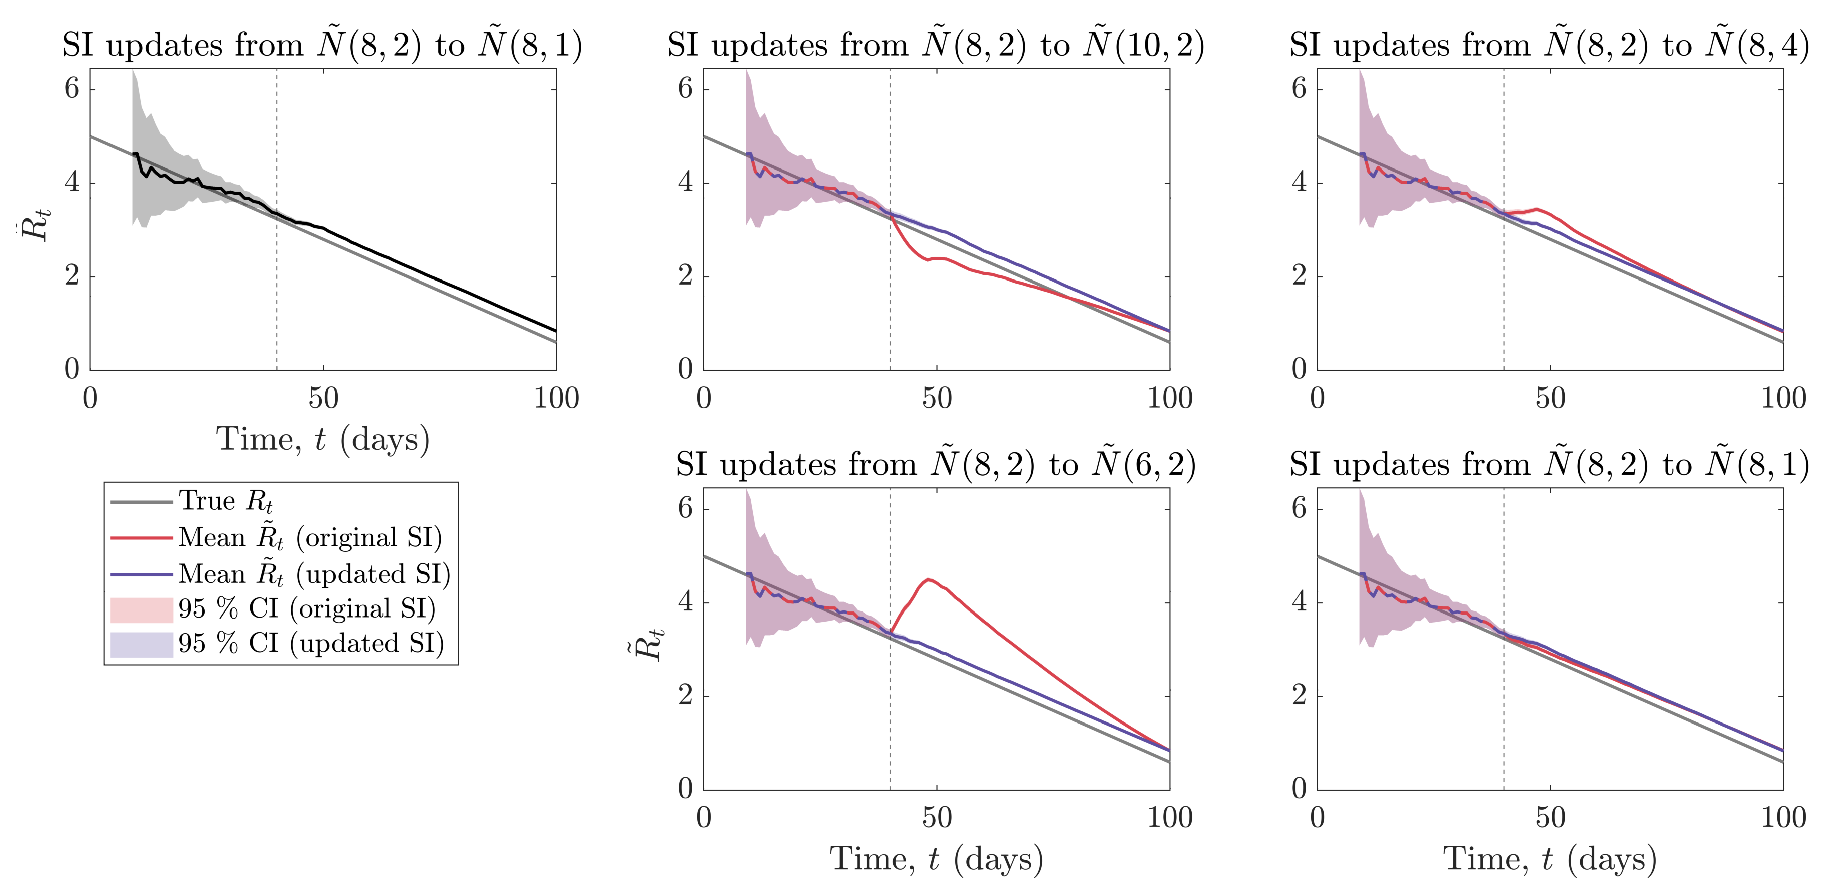
\includegraphics[width=\linewidth]{Figures/Report_Vary_Lin_Decrease_R_Disc_Serial_All.eps}
\captionof{figure}{}
\label{fig:Vary_Lin_Decrease_R_Disc_Serial_All}
\end{figure*}

However, figures \ref{fig:Vary_Lin_Increase_R_Disc_Serial_1} - \ref{fig:Vary_Lin_Increase_R_Disc_Serial_4} demonstrate an alternative 
narrative. These simulations attempt to re-infer an $R_t$ that is increasing in time. Here we find that the inferences do not converge and critically the inference  gets worse with time, so that the rate at which $R_t$ is increasing is incorrectly estimated.

\begin{figure*}
\centering
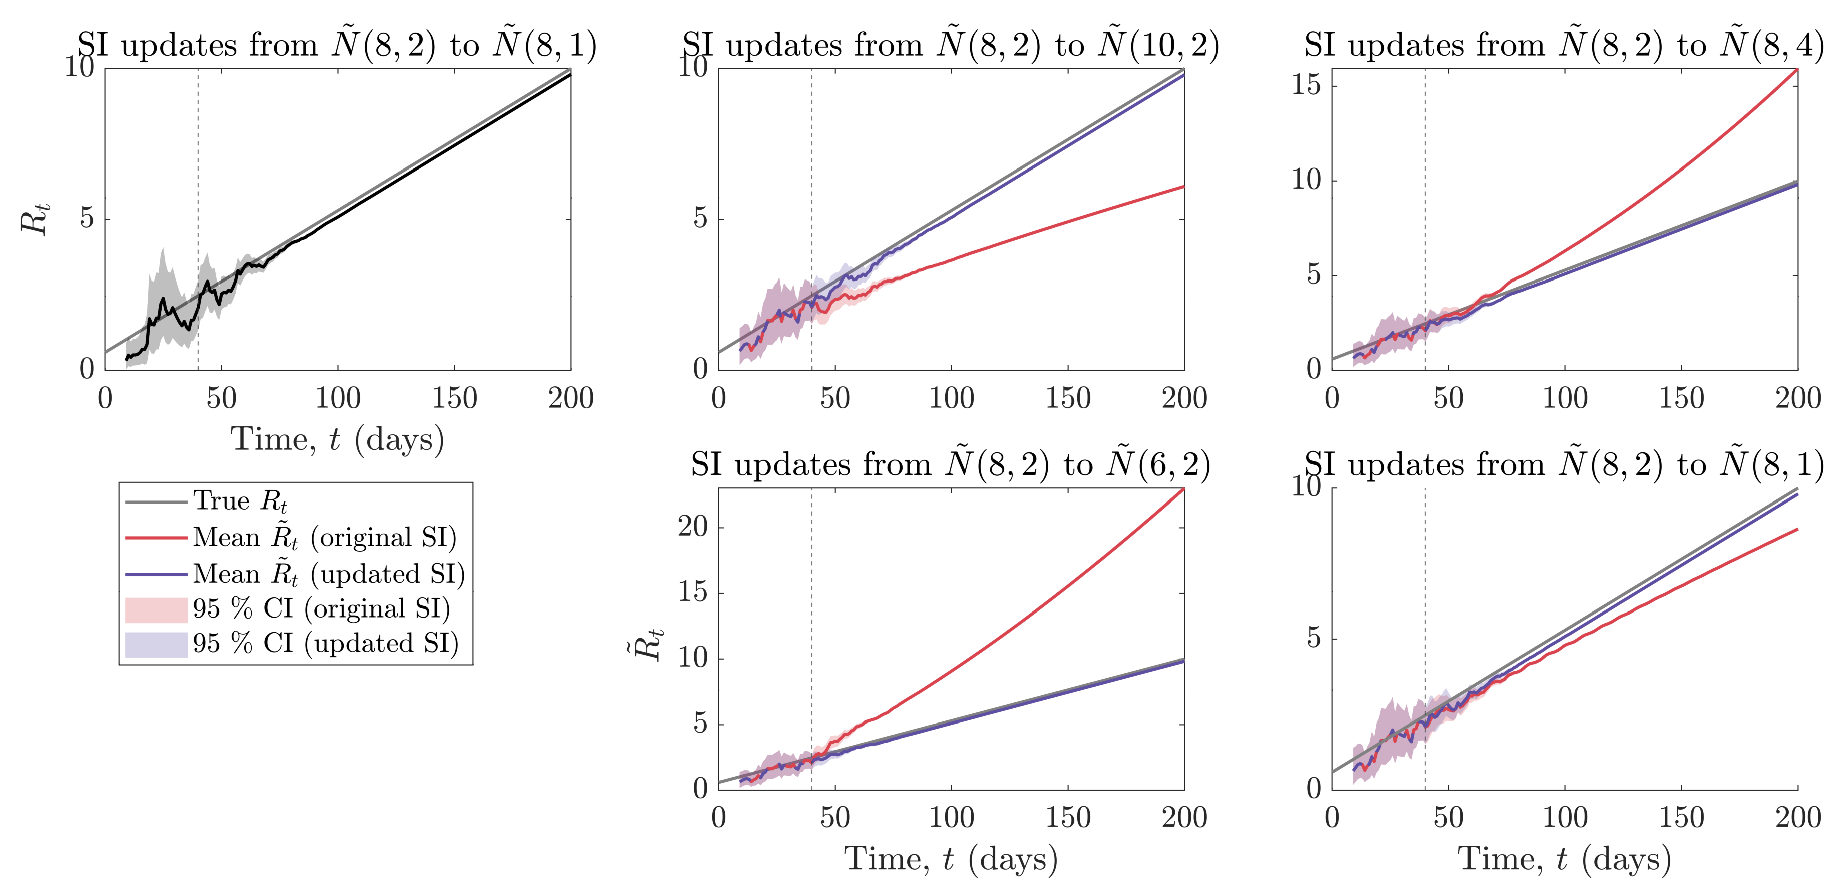
\includegraphics[width=\linewidth]{Figures/Report_Vary_Lin_Increase_R_Disc_Serial_All.eps}
\captionof{figure}{}
\label{fig:Vary_Lin_Decrease_R_Disc_Serial_All}
\end{figure*}

% \begin{minipage}{\linewidth}
% \centering
% 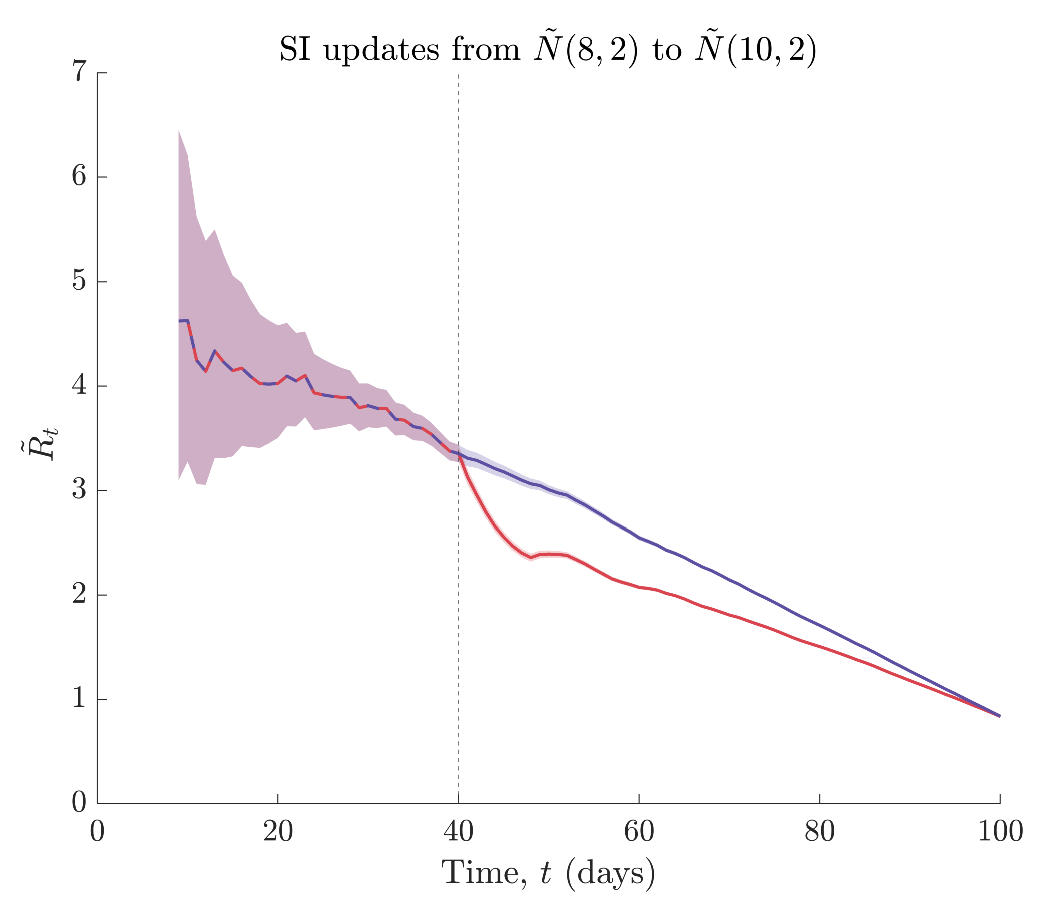
\includegraphics[width=\linewidth]{Figures/Report_Vary_Lin_Decrease_R_Disc_Serial_1.eps}
% \captionof{figure}{}
% \label{fig:Vary_Lin_Decrease_R_Disc_Serial_1}
% \end{minipage}

% \begin{minipage}{\linewidth}
% \centering
% 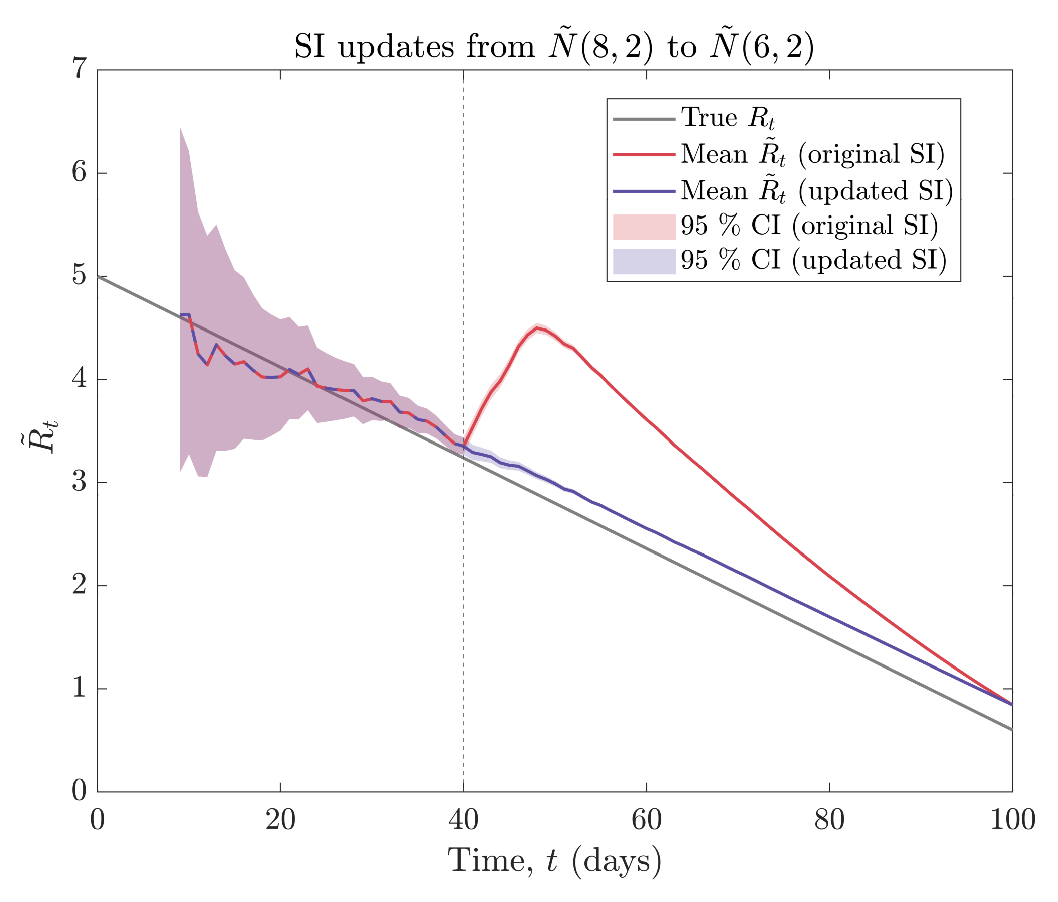
\includegraphics[width=\linewidth]{Figures/Report_Vary_Lin_Decrease_R_Disc_Serial_2.eps}
% \captionof{figure}{}
% \label{fig:Vary_Lin_Decrease_R_Disc_Serial_2}
% \end{minipage}

% \begin{minipage}{\linewidth}
% \centering
% 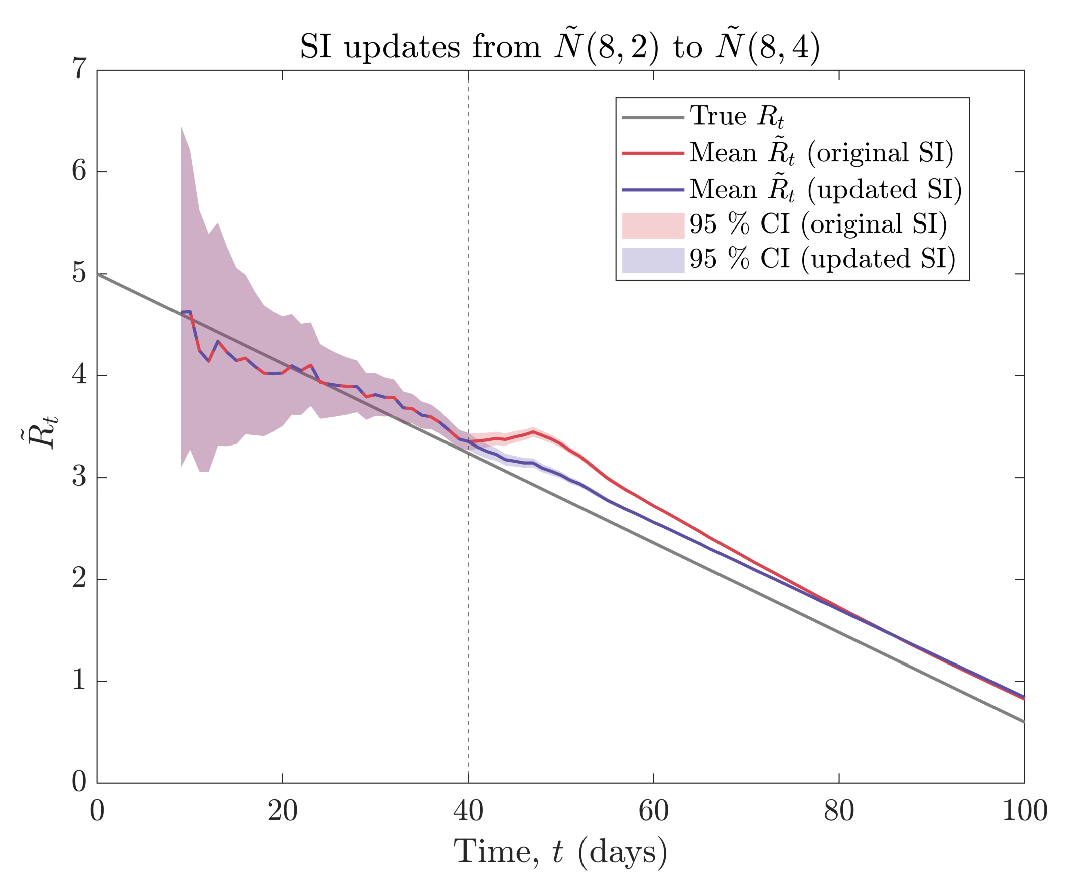
\includegraphics[width=\linewidth]{Figures/Report_Vary_Lin_Decrease_R_Disc_Serial_3.eps}
% \captionof{figure}{}
% \label{fig:Vary_Lin_Decrease_R_Disc_Serial_3}
% \end{minipage}

% \begin{minipage}{\linewidth}
% \centering
% 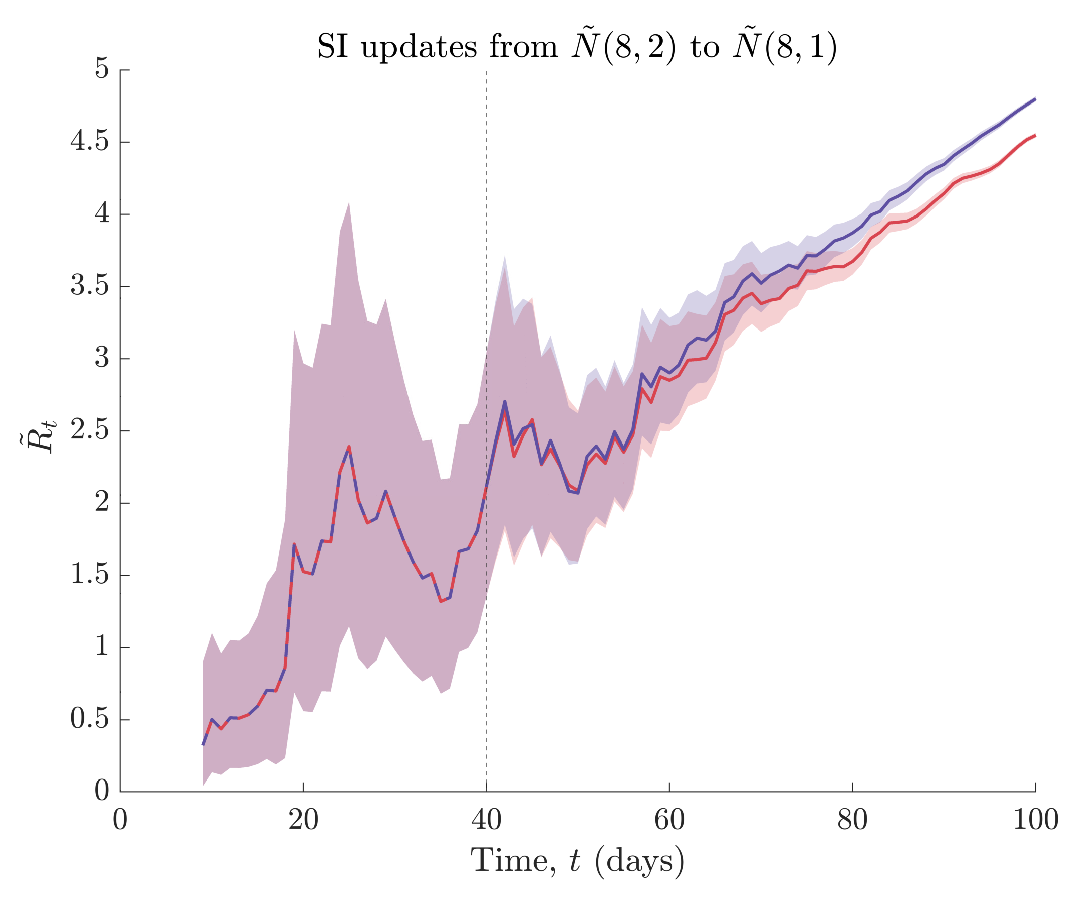
\includegraphics[width=\linewidth]{Figures/Report_Vary_Lin_Increase_R_Disc_Serial_4.eps}
% \captionof{figure}{}
% \label{fig:Vary_Lin_Decrease_R_Disc_Serial_4}
% \end{minipage}




% \begin{minipage}{\linewidth}
% \centering
% 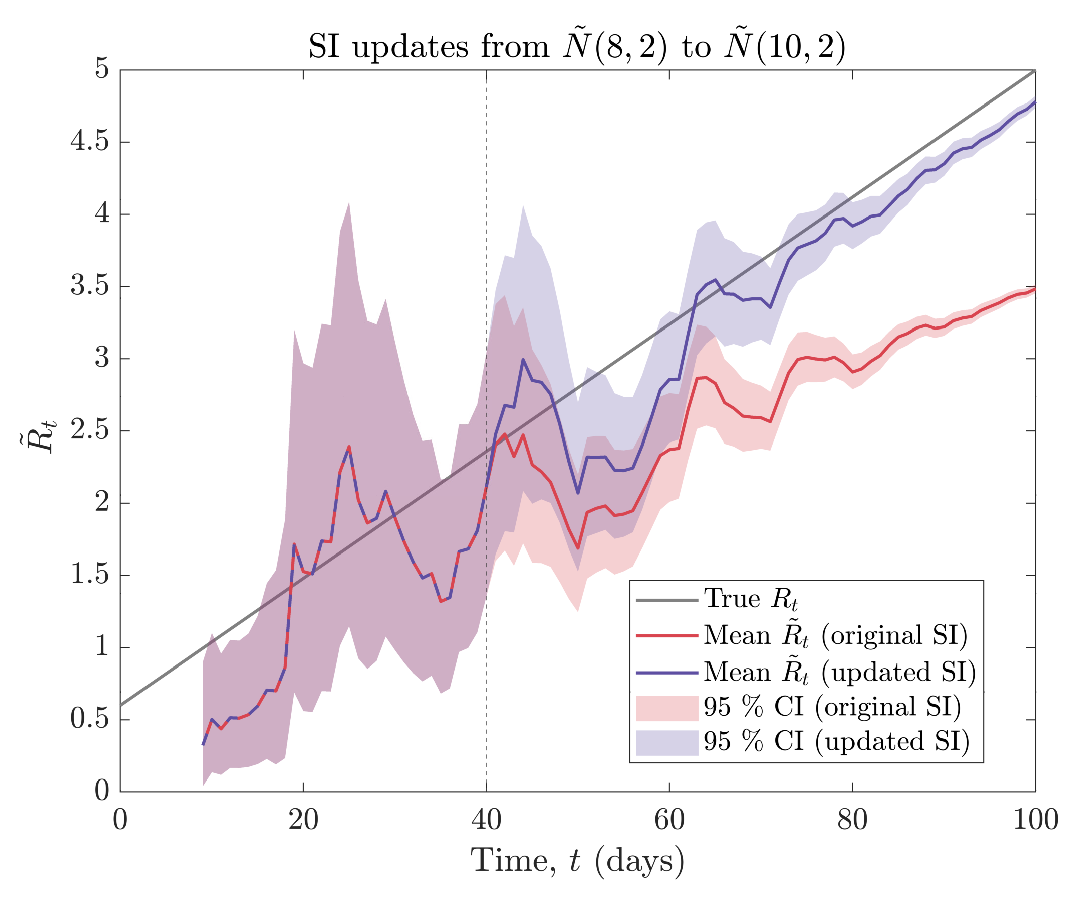
\includegraphics[width=\linewidth]{Figures/Report_Vary_Lin_Increase_R_Disc_Serial_1.eps}
% \captionof{figure}{}
% \label{fig:Vary_Lin_Increase_R_Disc_Serial_1}
% \end{minipage}

% \begin{minipage}{\linewidth}
% \centering
% 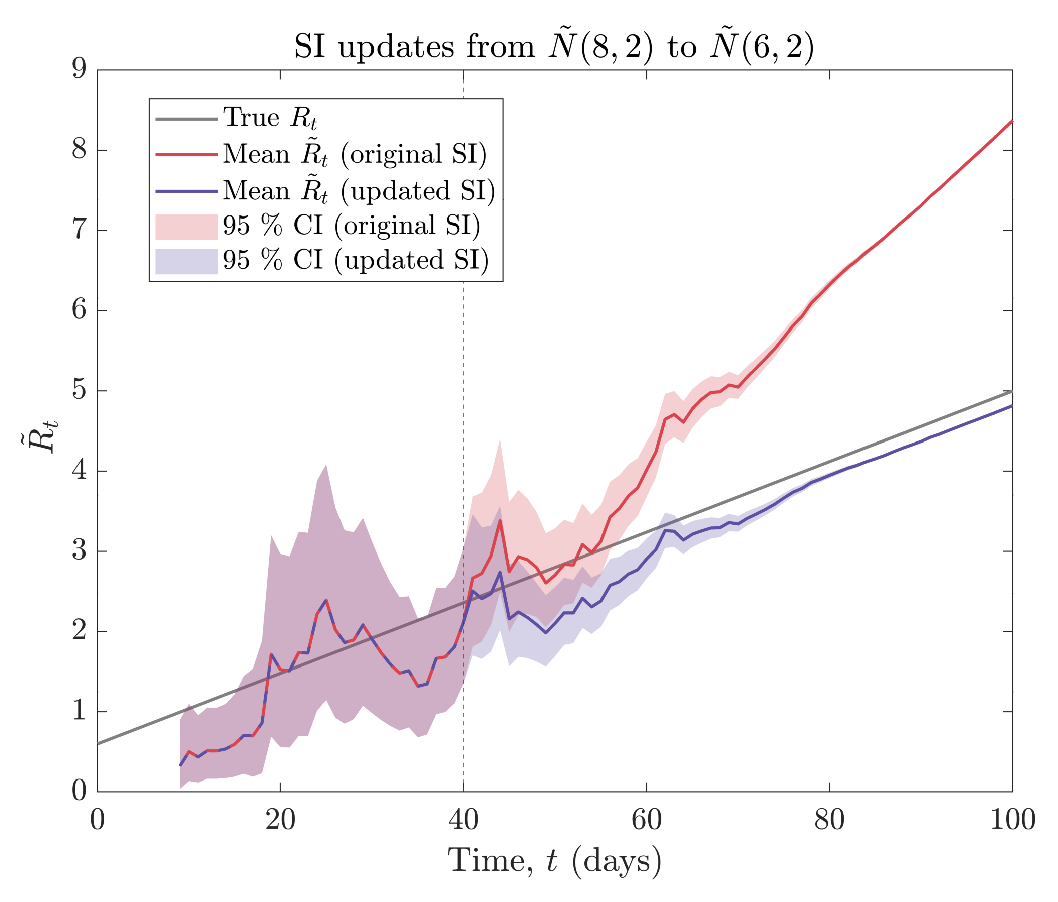
\includegraphics[width=\linewidth]{Figures/Report_Vary_Lin_Increase_R_Disc_Serial_2.eps}
% \captionof{figure}{}
% \label{fig:Vary_Lin_Increase_R_Disc_Serial_2}
% \end{minipage}

% \begin{minipage}{\linewidth}
% \centering
% 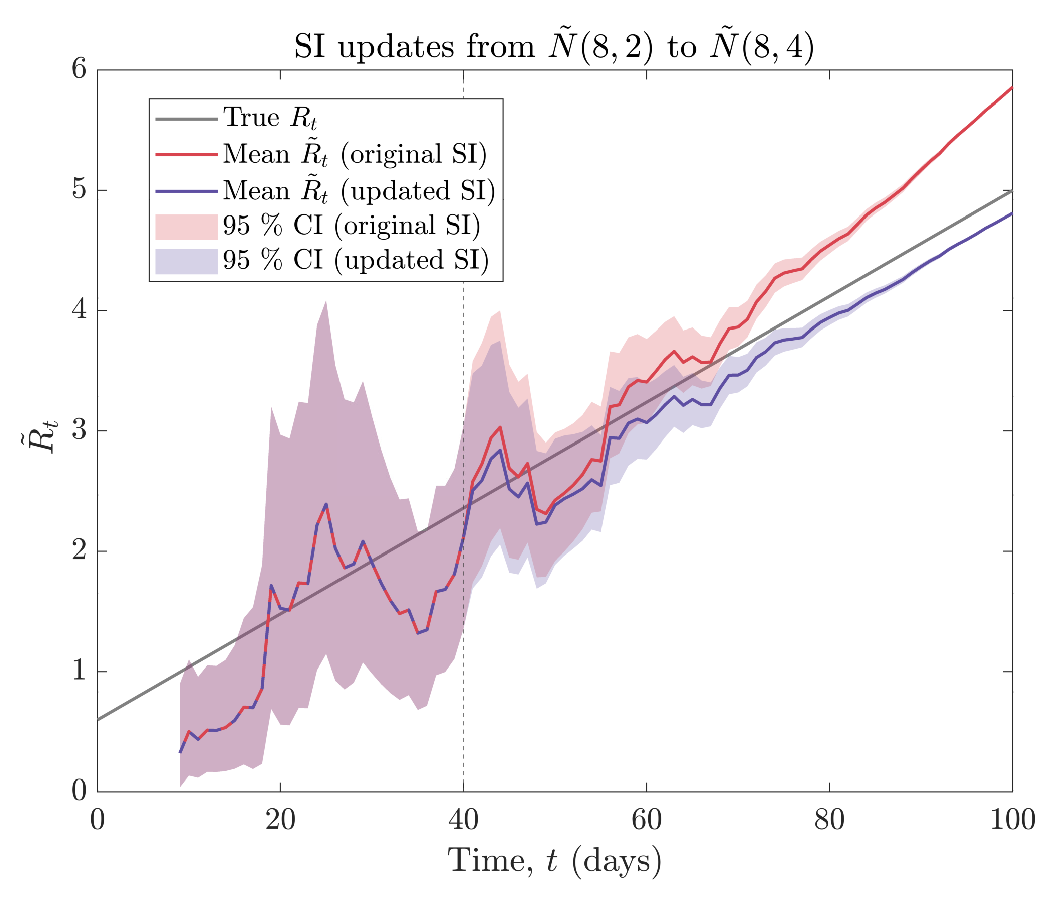
\includegraphics[width=\linewidth]{Figures/Report_Vary_Lin_Increase_R_Disc_Serial_3.eps}
% \captionof{figure}{}
% \label{fig:Vary_Lin_Increase_R_Disc_Serial_3}
% \end{minipage}

% \begin{minipage}{\linewidth}
% \centering
% 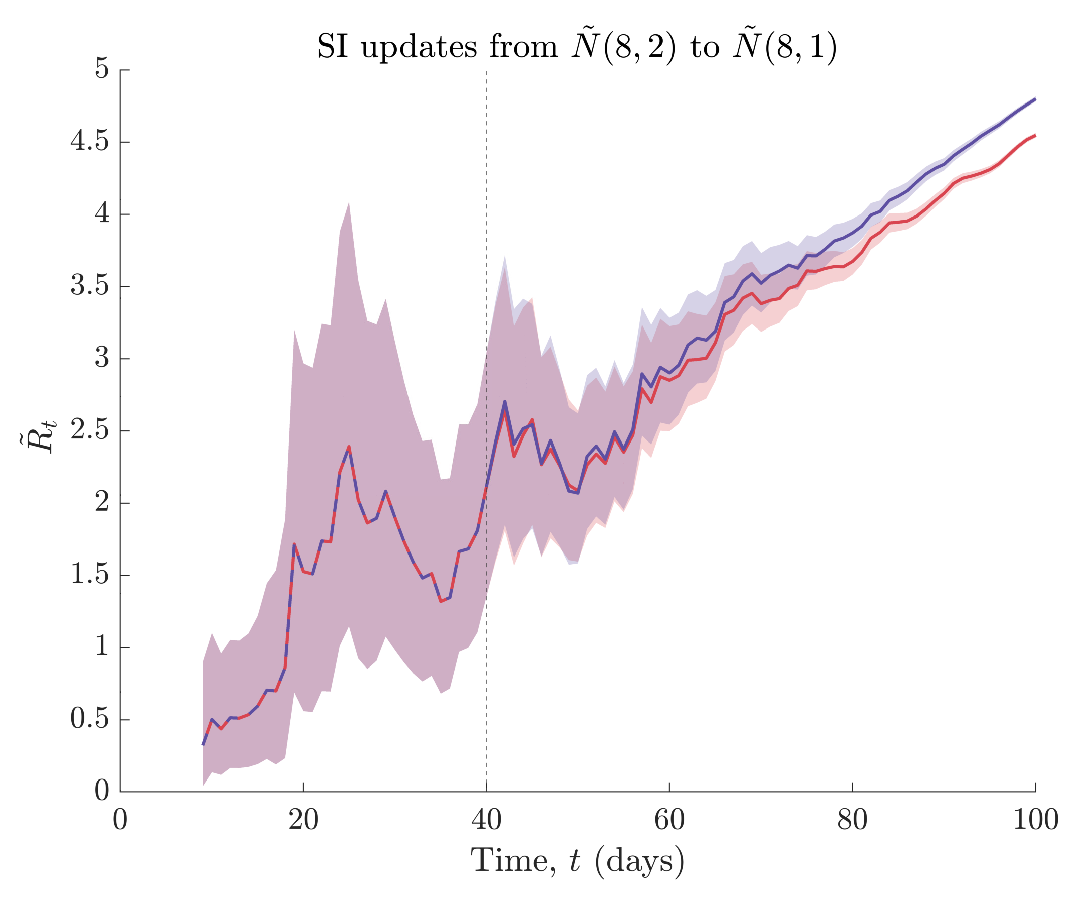
\includegraphics[width=\linewidth]{Figures/Report_Vary_Lin_Increase_R_Disc_Serial_4.eps}
% \captionof{figure}{}
% \label{fig:Vary_Lin_Increase_R_Disc_Serial_4}
% \end{minipage}

\subsubsection{Sensitivity Analysis}\label{sect::Sens_Linear_R}

We have identified what we believe to be trends in the inference of $R_t$. We now present sensitivity analyses to confirm these trends and suggest several nuances to our findings.

\begin{minipage}{\linewidth}
\centering
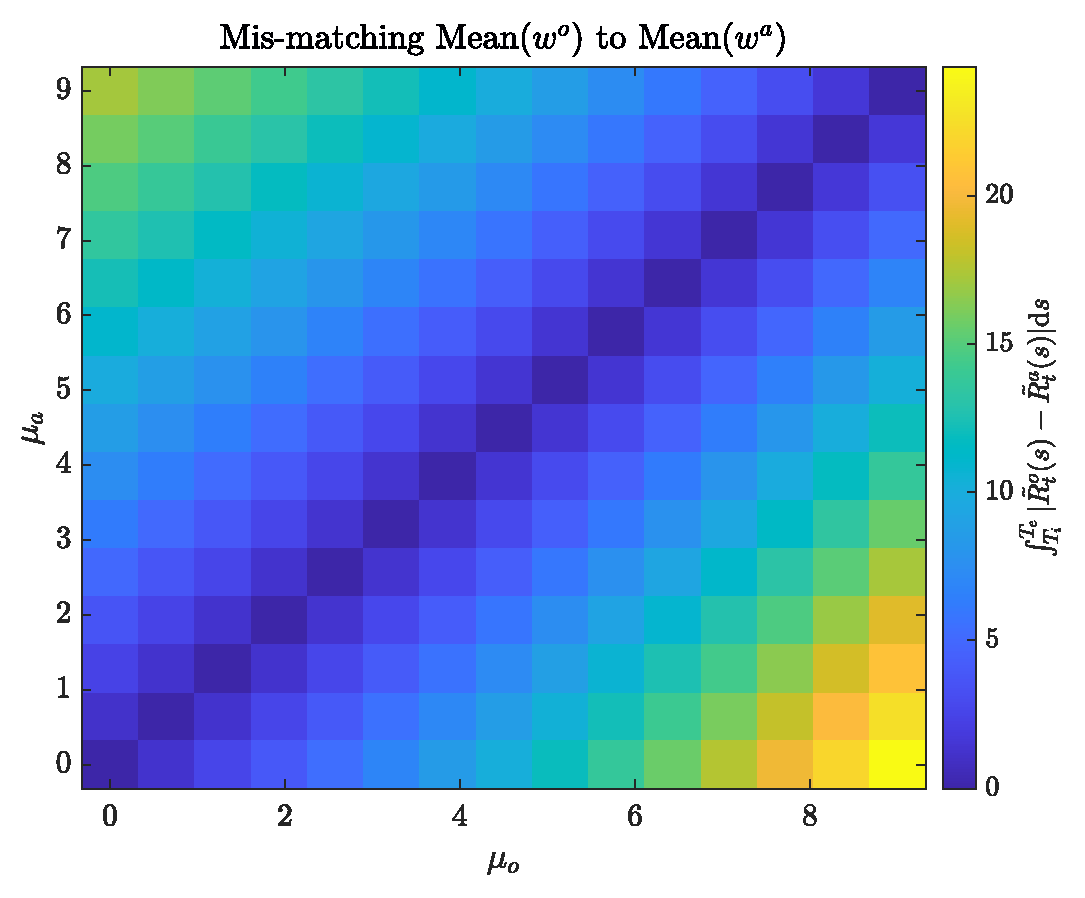
\includegraphics[width=\linewidth]{Figures/Area_Sensitivity_to_Mean_SI_Decreasing_R_t.eps}
\captionof{figure}{}
\label{fig:Vary_Lin_Increase_R_Disc_Serial_4}
\end{minipage}

\begin{minipage}{\linewidth}
\centering
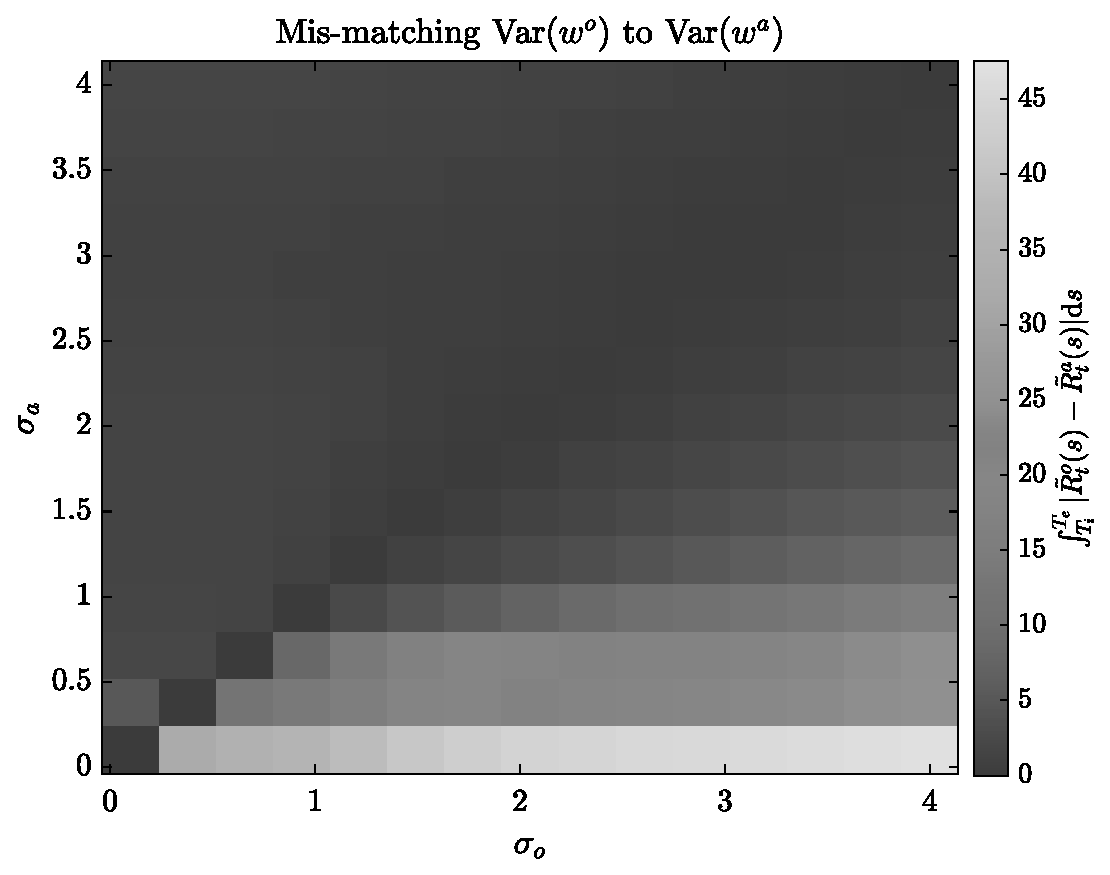
\includegraphics[width=\linewidth]{Figures/Area_Sensitivity_to_Std_SI_Decreasing_R_t.eps}
\captionof{figure}{}
\label{fig:Vary_Lin_Increase_R_Disc_Serial_4}
\end{minipage}

\begin{minipage}{\linewidth}
\centering
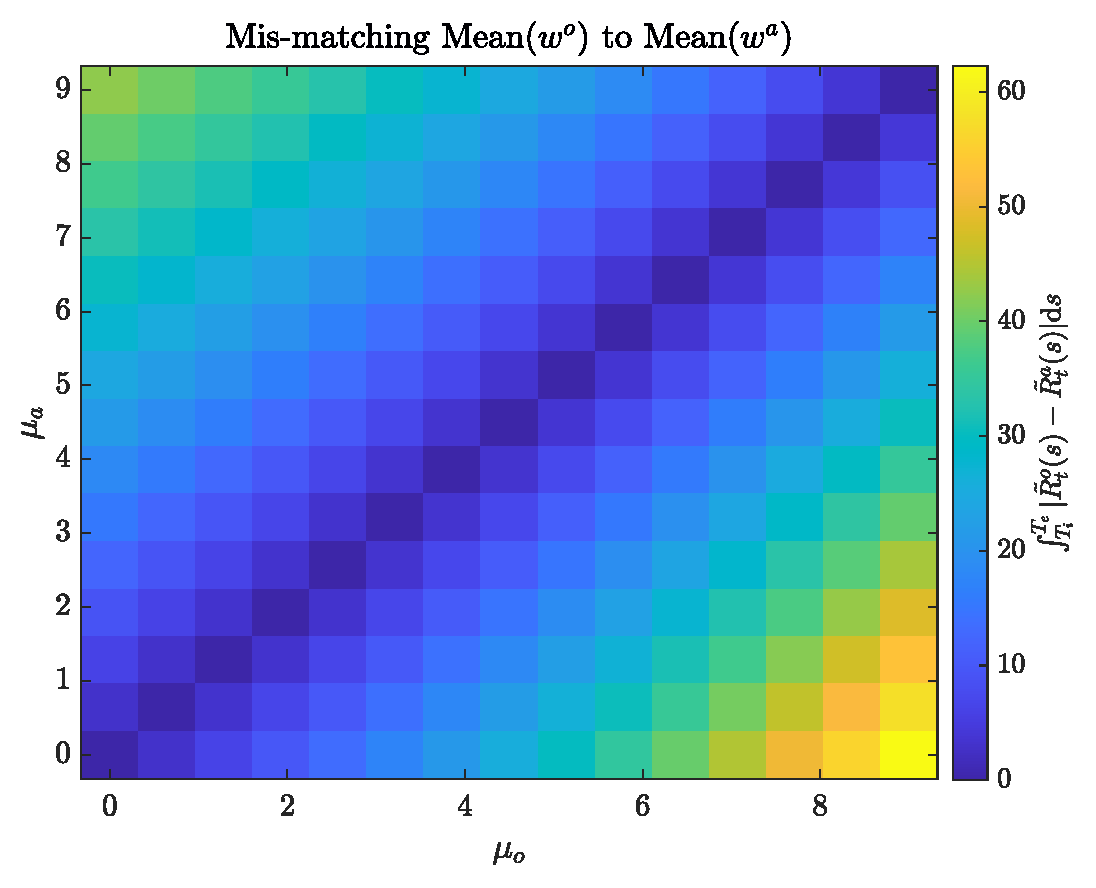
\includegraphics[width=\linewidth]{Figures/Area_Sensitivity_to_Mean_SI_Increasing_R_t.eps}
\captionof{figure}{}
\label{fig:Vary_Lin_Increase_R_Disc_Serial_4}
\end{minipage}

\begin{minipage}{\linewidth}
\centering
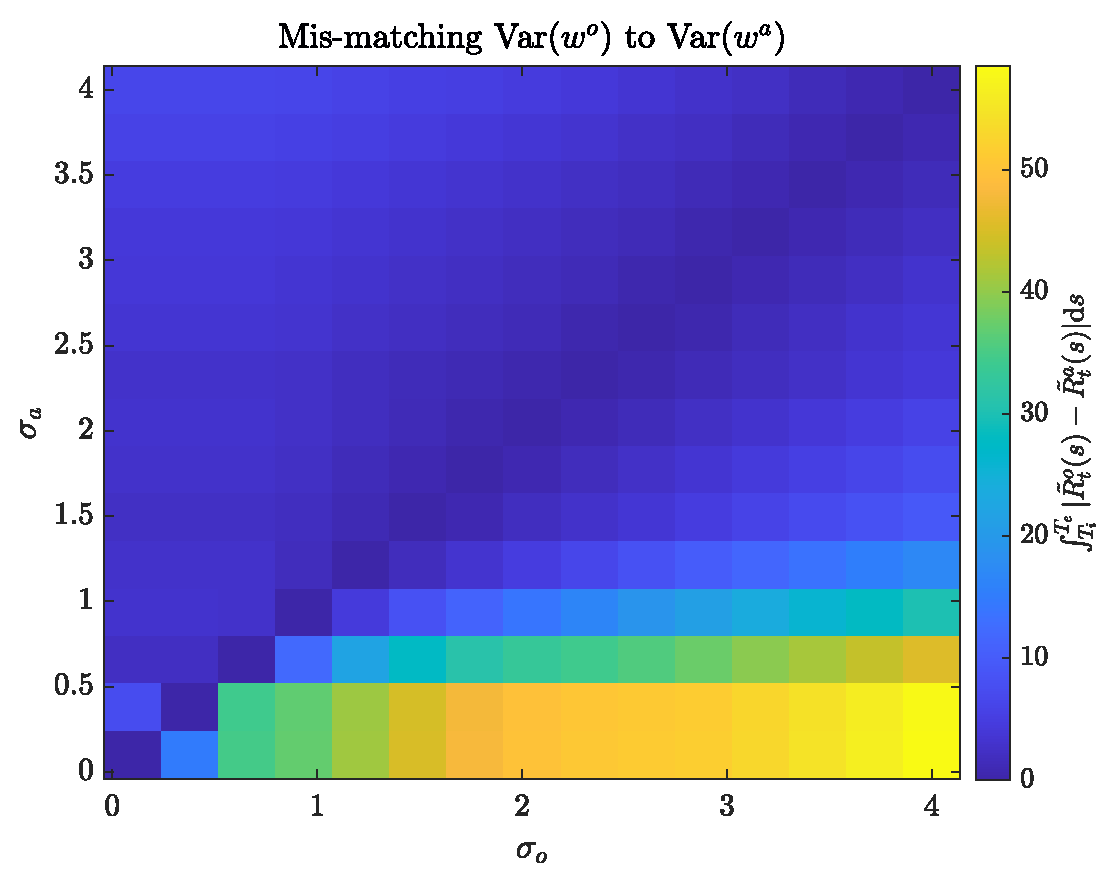
\includegraphics[width=\linewidth]{Figures/Area_Sensitivity_to_Std_SI_Increasing_R_t.eps}
\captionof{figure}{}
\label{fig:Vary_Lin_Increase_R_Disc_Serial_4}
\end{minipage}

\begin{minipage}{\linewidth}
\centering
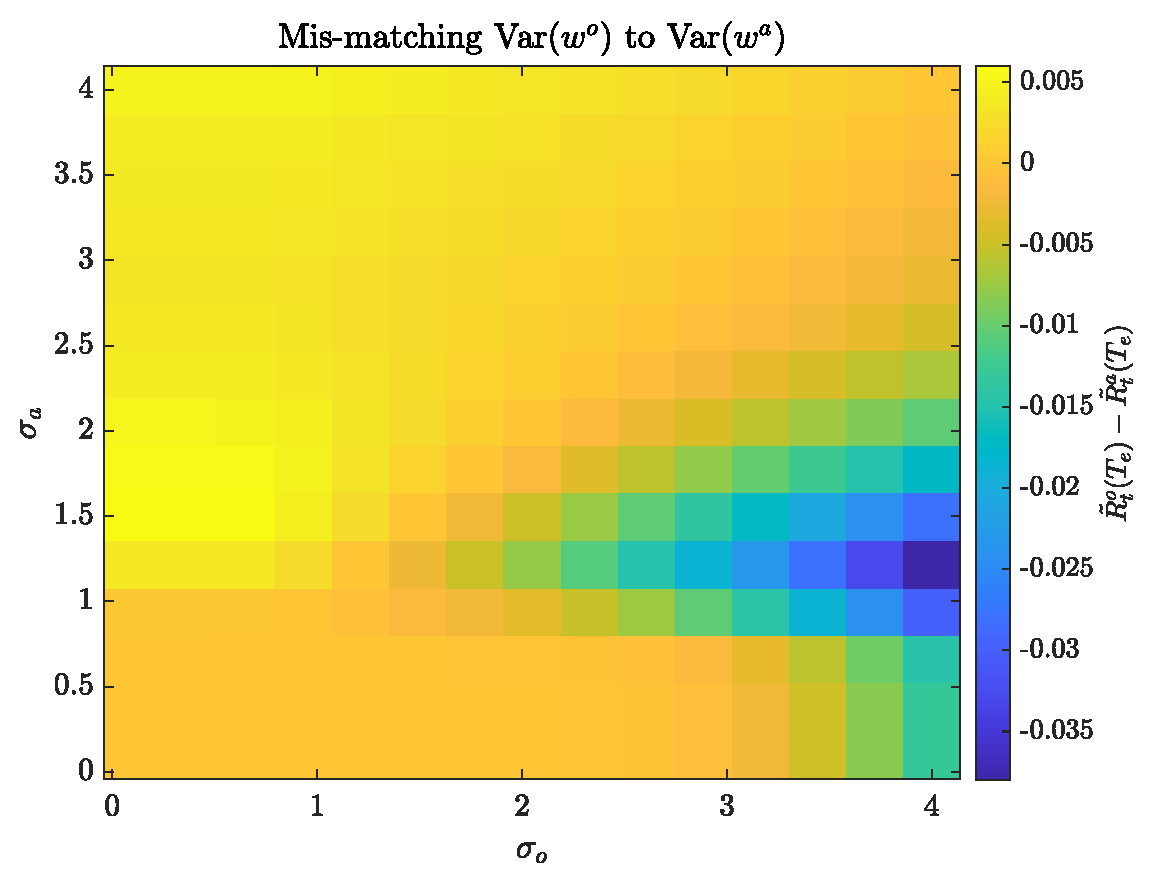
\includegraphics[width=\linewidth]{Figures/Mean_Sensitivity_to_Std_SI_Decreasing_R_t.eps}
\captionof{figure}{}
\label{fig:Vary_Lin_Increase_R_Disc_Serial_4}
\end{minipage}

\begin{minipage}{\linewidth}
\centering
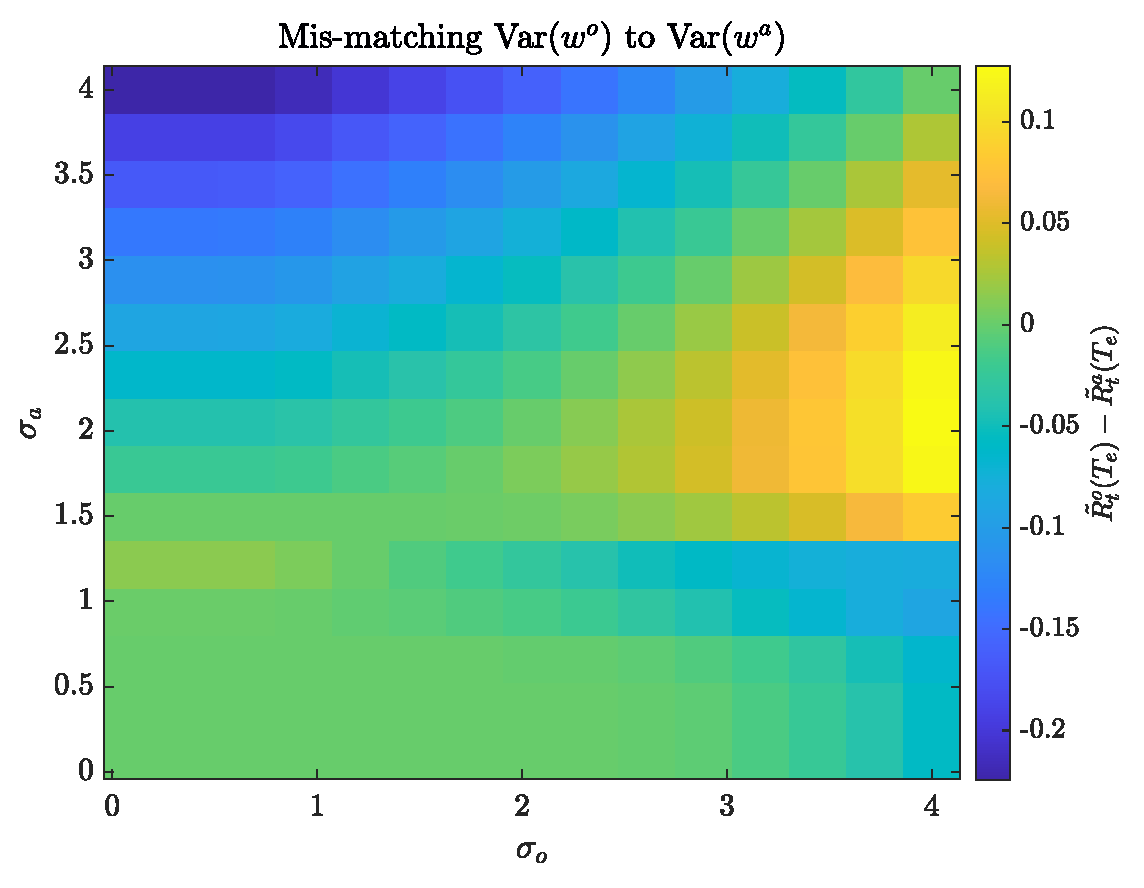
\includegraphics[width=\linewidth]{Figures/Mean_Sensitivity_to_Std_SI_Increasing_R_t.eps}
\captionof{figure}{}
\label{fig:Vary_Lin_Increase_R_Disc_Serial_4}
\end{minipage}




\subsection{Effect of not truncating the serial interval on $R_t$}

\subsubsection{Problem framework}
Here, I investigate analytically the impact of using a serial interval, $w_s^o$ (original) with domain length $N_o$ from the early stages of a pandemic instead of the ideal $w_s^a$ (actual) with domain length $N_t$. This is highly relevant since there are often quarantining control measures for individuals who test positive during an epidemic. \\If the data collection for the serial interval is prior to these statutory laws being introduced, it is highly likely the serial interval should be over a truncated domain of the original SI. We make the assumption here that the actual serial interval, $w_s^a$ only changes in terms of domain so that $N_t <N_o$. In reality, the actual serial interval may involve other transformations from the original SI but here we solely consider this alteration.\\

\subsubsection{Relative $R_t$ set-up}
Our model assumes that $$ R_t = \frac{I_t^{\text{local}}}{ \Lambda_t(w_s)}$$ and so to consider the effect of not truncating the serial interval on $R_t$, we should consider whether
\begin{align}
\frac{R_t^o}{R_t^a} &\mathop{\lessgtr} 1 \text{, i.e.} \notag\\
\frac{\Lambda_t(w_s^a)}{\Lambda_t(w_s^o)} &\mathop{\lessgtr} 1 
\end{align}
This quantity will determine whether or not the $R_t^o$ is an over-estimate or under-estimate.
\subsubsection{Normalisation of new serial interval}
So long as the the original SI with domain $(0, \cdots N_o)$ is given and we consider a actual domain $(0, \cdots, N_r)$ s.t $N_r<N_o$, the new, truncated serial interval is already prescribed since the PMF must sum to 1.\\
First we let
\begin{equation} \label{eq:ap2}
\alpha = \sum^{N_o}_{k &= N_r +1}w_k^o    
\end{equation}

and therefore
$$ \sum^{N_r}_{k=0}w_k^o &= 1- \alpha. $$
Since we keep the shape of $w_s^a$ the same over the truncated domain, i.e.
$$w_k^a = \beta w_k^o \text{ for } k = 0, \cdots N_r.$$
But by the summation requirement on the real serial interval:
\begin{align*}
1 = \sum_{k=0}^{N_r}w_k^a  &= \beta \sum_{k=0}^{N_r}w_k^o \\
&= \beta (1-\alpha)\\
\implies w_k^a &= \frac{w_k^o}{1-\alpha} \text{ for } k = 0, \cdots N_r.
\end{align*}

\subsubsection{Over/Under Estimation result}

We note (given our definition of $\alpha$) the existence of two quantities of interest, $\hat{I}_t$ and $\tilde{I}_t$

\begin{align}
    \alpha \hat{I}_t &= \sum^{N_o}_{k =N_r+1} I_{t-k}w_k^o \text{ and }\label{eq:ap3}\\
    (1-\alpha)\tilde{I}_t &= \sum^{N_r}_{k =0} I_{t-k}w_k^o \label{eq:ap4}
\end{align}
Effectively, $\hat{I}_t$ and $\tilde{I}_t$ group the contributions to the original $R_t$ estimate for the original SI (extra-truncated and un-truncated respectively). We now show that it is the ratio of these two quantities that determine the over/under-estimation quantity of $R_t^o$.\\

NB: The equation for $\tilde{I}_t$ can be further reduced to 

\begin{equation} \label{eq:ap1}
\tilde{I}_t = \sum^{N_r}_{k =0} I_{t-k}w_k^a
\end{equation}
Referring back to the reciprocal of the estimation quantity gives

\begin{align*}
    \kappa = \frac{R_t^a}{R_t^o} &= \frac{\sum^{N_o}_{k=0}I_{t-k}w_k^o}{\sum^{N_r}_{k=0}I_{t-k}w_k^a}\\
    &= \frac{\sum^{N_r}_{k=0}I_{t-k}w_k^o + \alpha \hat{I}_t}{\tilde{I}_t} \text{ by (\ref{eq:ap1}) and (\ref{eq:ap2}) }\\
    &= \frac{(1-\alpha)\tilde{I}_t +\alpha \hat{I}_t}{\tilde{I}_t} \text{ by (\ref{eq:ap4})}\\
    &= 1 +\alpha \left(\frac{\hat{I}_t}{\tilde{I}_t}-1 \right)
\end{align*}
It is easy to verify that $\frac{R_t^a}{R_t^o} \in (0, \infty)$ but crucially, we note that if $\kappa>1$ (equivalently $\hat{I}_t>\tilde{I}_t$), $R_t^o$ is an under-estimate and if $\kappa<1$ (equivalently $\hat{I}_t<\tilde{I}_t$), $R_t^o$ is an over-estimate.


$\hat{I}_t> \tilde{I}_t \implies R_t^o>R_t^a$ and conversely $\hat{I}_t< \tilde{I}_t \implies R_t^o<R_t^a$.

\newpage
\subsection{Effect of differing mean and variance of recorded serial interval on $R_t$ inference}

From the previous section in the Appendix, we deduced that

\begin{equation} \label{eq:R_t_ratio}
\frac{\tilde{R}_t^o}{\tilde{R}_t^a} = \frac{\sum_{i=1}^{N}I_{t-i}w_i^a}{\sum_{i=1}^{N}I_{t-i}w_i^o},
\end{equation}
where $N$ is the length of both the original and actual serial intervals (this time the length is not truncated). Note that the quantity in (\ref{eq:R_t_ratio}) is the ratio of \textit{inferred} $R_t$ values and will inform us on whether we are over/under-estimating the reproduction number, and by how much.\\
Let us define both

  \begin{align*}
    \boldsymbol{v}(r) &= \begin{bmatrix}
           e^{-r} \\
           e^{-2r} \\
           \vdots \\
           e^{-Nr}
         \end{bmatrix} \text{ and}\\
         \boldsymbol{\Delta} &= \boldsymbol{w}^a-\boldsymbol{w}^o,
  \end{align*}
  
where $\boldsymbol{w}^o$ and $\boldsymbol{w}^a$ are the original and actual (after the original serial interval is updated) serial intervals respectively.\\
The reader should note that (as we will make clear soon) that $r$ is the \textit{epidemic growth rate} \textbf{find reference}. \footnote{Throughout this analysis, we will refer to both $R_t$ and $r$ interchangeably (the exact relationship has been discussed thoroughly in \cite{Wallinga-Lipsitch}, which we make reference to later) but crucially $R_t>1$ if and only if $r>0$, whilst $R_t<1$ if and only if $r<0$.}
Equation (\ref{eq:R_t_ratio}) shows that we are interested in understanding what happens to $R_t$ inference when the original serial interval is used, instead of the updated (actual) serial interval.\\
Crucially, we note that $\boldsymbol{v}(r)$ is not necessarily orthogonal to $\boldsymbol{\Delta}$. The importance behind this relationship will become clear during this section. \footnote{Discussing the existence of a non-zero $r$ that makes $\boldsymbol{v}(r)$ orthogonal will form a large part of our analysis.}

Suppose we know the following:

\begin{itemize}
    \item whether or not $\mu_a \mathop{\lessgtr} \mu_o $ (and $\sigma_a \mathop{\lessgtr} \sigma_o$ although as we shall see the variance of the interval becomes obsolete),
    \item $\delta$, the number of sequential sign changes in $\boldsymbol{\Delta}$,
    \item the incidence data is `well-behaved', i.e. $I_t = p+qe^{rt}$ and we will assume that $p$ and $q$ are both positive (although there may be examples where this is not a necessary condition.)
\end{itemize}

We choose this form for $I_t$ because, for a constant $R_t$ and the data-generation method that we have described in Section \ref{sect:Method}, we expect exponential growth/decay for $R_t>1$ ($r>0$) or $R_t<1$ ($r<0$) respectively.\\

Taking this assumption, we can express equation \ref{eq:R_t_ratio} in terms of the `Discrete Laplace transforms',  $$ L_{\{o, a\}}(x) = \sum_{i=1}^{N}e^{-ix}w_i^{\{o, a\}}$$ of the two serial intervals as follows:\\
Let
\begin{align}
h(r) &= \frac{\tilde{R}_t^o}{\tilde{R}_t^a} \notag\\
&= \frac{p + q\sum_{i=1}^N e^{r(t-i)}w_i^a}{p + q\sum_{i=1}^N e^{r(t-i)}w_i^o} \notag\\
&= \frac{p+qe^{rt}L_a(r)}{p+qe^{rt}L_o(r)} \notag\\ 
&= \frac{p+qe^{rt}L_a(r)}{p+qe^{rt}L_o(r)} \label{eq:R_t_ratio2}
\end{align}\\
The focus of this analysis is to know the shape of this graph (this will enable us to determine over/under-estimates) although we might suspect it is dependent on $\boldsymbol{\Delta}$.\\ It is particularly significant to identify when $h(r) = 1$, since this implies that despite having different SIs, the $R_t$-inference is unaffected. Equation (\ref{eq:R_t_ratio2}) combined with $$ \boldsymbol{w}^a \cdot \boldsymbol{1} = \boldsymbol{w}^o \cdot \boldsymbol{1}=0$$ imply that $h(0) = 1$, i.e. when $R=1$ (the growth rate, $r$ is null), the inference will always be the same regardless of the serial interval used.\\
Similarly 
$$\lim_{r \rightarrow -\infty}h(r)=1 \text{ provided }p \neq 0.$$

\begin{align*}
    \lim_{r \rightarrow -\infty}h(r)&=1 \text{ provided }p \neq 0.\\
    \lim_{r \rightarrow +\infty}h(r)&=\frac{w_1^a}{w_1^o} \text{ provided both }p \neq 0 \text{ and }w_1^o \neq 0 \neq w_1^a.
\end{align*}

To be rigorous, we should consider the converse, i.e. consider $h(r) = 1$ and infer $r$-values. We suggest a relatively weak assumption on the serial interval shift, $\boldsymbol{\Delta}$ that generates a strong conclusion, but also discuss another class of SIs which are harder to analyse and also exhibit slightly more complicated behaviour. The framework for this problem will be solving $h(r) = 1$ for $r$, subject to different $\boldsymbol{\Delta}$ shifts. Taking this framework with our original equation \ref{eq:R_t_ratio2}, we can reduce the problem to solving: 
\begin{align}
   qe^{rt}\sum_{j=1}^{N} e^{-jr}\Delta_j &= 0 \notag \\
   \implies qe^{r(t-1)}\sum_{j=1}^{N} e^{r(1-j)}\Delta_j &= 0 \label{eq:Key}
\end{align}
for $r$.\\
We can factor out the $qe^{r(t-1)}$ term since this is non zero for finite $r$. Note that we are now considering which values of $r$ force $\boldsymbol{v}(r) \cdot \boldsymbol{\Delta}=0$.

If we now let $z = e^{-r}$ (noting that this forces $z>0$), we retrieve
\begin{equation}\label{eq:Poly}
    \Delta_1 +\Delta_2 z + \cdots +\Delta_{N}z^{N-1} = 0.
\end{equation}



Equation (\ref{eq:Key}) preserves solutions with $r=0$ and $r=-\infty$. We now split the discussion into two separate cases, based on the number of sign-changes in $\boldsymbol{\Delta}$. \textbf{Define sign changes!}

\textit{Descartes's Rule of Signs} states that ``the number of positive real zeros of $p(x)$ (counted with multiplicities) is either equal to the number of variations in sign in the sequence $a_0, \cdots a_n$ of the coefficients or less than that by an even whole number.'' We state this without proof but a simple proof is available \textbf{here}.

\subsubsection*{$\boldsymbol{\Delta}$ with 1 sign-change ($\delta = 1$)}

Let $\exists j \in \{ 1, \cdots,  N \}$ (with $\mathrm{sgn}(\Delta_j) \neq 0$) s.t.

\begin{equation}
  \mathrm{sgn}(\Delta_i) =
    \begin{cases}
      \mathrm{sgn}(\Delta_j) & \text{for } i \leq j\\
      -\mathrm{sgn}(\Delta_j) & \text{for } i > j
    \end{cases}       
\end{equation}

It follows from \textit{Descartes's Rule of Signs} that since there is always one root at $z=1$, and there is exactly one sign change in the coefficients of the polynomial, that this root is the \textit{only} root for $z>0$. Since roots that are negative do not correspond to real $c$ values, we can conclude that $h(c) = 1 \iff c = 0$ when $\Delta$ has exactly one sign change. While this assumption seems strong, the vast majority of serial interval updates will follow this pattern, especially if they are updates from the same distribution.

\subsubsection*{$\boldsymbol{\Delta}$ with 2 sign-changes ($\delta = 2$)}

Let $\exists k, j (k>j) \in \{ 1, \cdots,  N \}$ (with $\mathrm{sgn}(\Delta_j) = -\mathrm{sgn}(\Delta_k) \neq 0 $) s.t.


\begin{equation}
  \mathrm{sgn}(\Delta_i) =
    \begin{cases}
      \mathrm{sgn}(\Delta_j) & \text{for } i \leq j \text{ or } i > k\\
      \mathrm{sgn}(\Delta_k) & \text{for } i \in \{ j+1, \cdots k \}
    \end{cases}       
\end{equation}

Similarly to the previous case, we can infer from \textit{Descartes's Rule of Signs} that there are exactly two positive roots, one at $z=1$ ($c = 0$) and another at $z>0$ ($c = c_1 \in \mathbb{R}$). This is because owing to DRS, there can only be zero or two real, positive roots, but once again there is always a root at $z=1$ by our set-up. It follows that there cannot be zero positive roots and so there must be two.\\

\subsubsection*{Discussion of $\delta$}

Technically, we could continue our analysis of $\delta$ values up to $N-1$ (since this is the maximum number of sign-changes in $\boldsymbol{\Delta}$). However this would be counter-productive for a number of reasons, namely:

\begin{itemize}
    \item An updated serial interval with three or more sign-changes is unlikely (or even mathematically impossible) if the serial intervals are estimated using the same distributions.
    \item Once there are three or more sign-changes, DRS tells us that we introduce ambiguity for how many roots to the polynomial in equation (\ref{eq:Poly}). For example, if there are three sign-changes, we can only deduce that there are either one or three $r$-values where the $R_t$ inference is true (in spite of an incorrect serial interval), which is not very illuminating.
\end{itemize}

One problem with implementing these findings is that even if we suppose $\boldsymbol{\Delta}$ is simple enough to have less than 3 sign changes, we do not know whether $\delta$ equals 1 or 2. The over/under-estimate behaviour is significantly different in both cases.

The consequence when $\delta=1$ is in line with previous analyses \textbf{what are these analyses?}. We will see that we can determine whether we are over/under-estimating $R_t$ by considering the sign of  $\mu_{\boldsymbol{\Delta}}$, $\Delta_1$ and $R_t-1 $. This is because $\delta$, $\mu_{\boldsymbol{\Delta}}$ and $\Delta_1$ are all we require to know the general shape of $h(r)$. An obvious problem is that we do not know any of these values exactly. Fortunately when $\delta=1$, $\mu_{\Delta}>0 \iff \Delta_1 <0$ \footnote{This is a surprising result. It means that if $\Delta_1$ and $\mu_{\boldsymbol{\Delta}}$ share the same sign, there cannot be exactly one sign change in $\Delta$.} (attempting to sketch $h(r)$ for $\mu_{\Delta}>0$ \& $\Delta_1>0$ or $\mu_{\Delta}<0$ \& $\Delta_1<0$ should convince the reader it is impossible). Therefore, if we suspect that $\delta=1$, we only require the sign of $R_t-1$ and the sign of either $\mu_\boldsymbol{\Delta}$ or $\Delta_1$ to give a quantitative remark about the inference.\\

Specifically, we can summarise the remarks when $\delta=1$ in Figure \ref{fig:Delta_Eq_1}, e.g. if $\mu_{\boldsymbol{\Delta}}<0$ and $R_t$ is known to be greater than one (i.e. $r$>0), then our $\tilde{R}_t$ will be an over-estimate of the true $R_t$.

\begin{minipage}{0.95\linewidth}
\centering
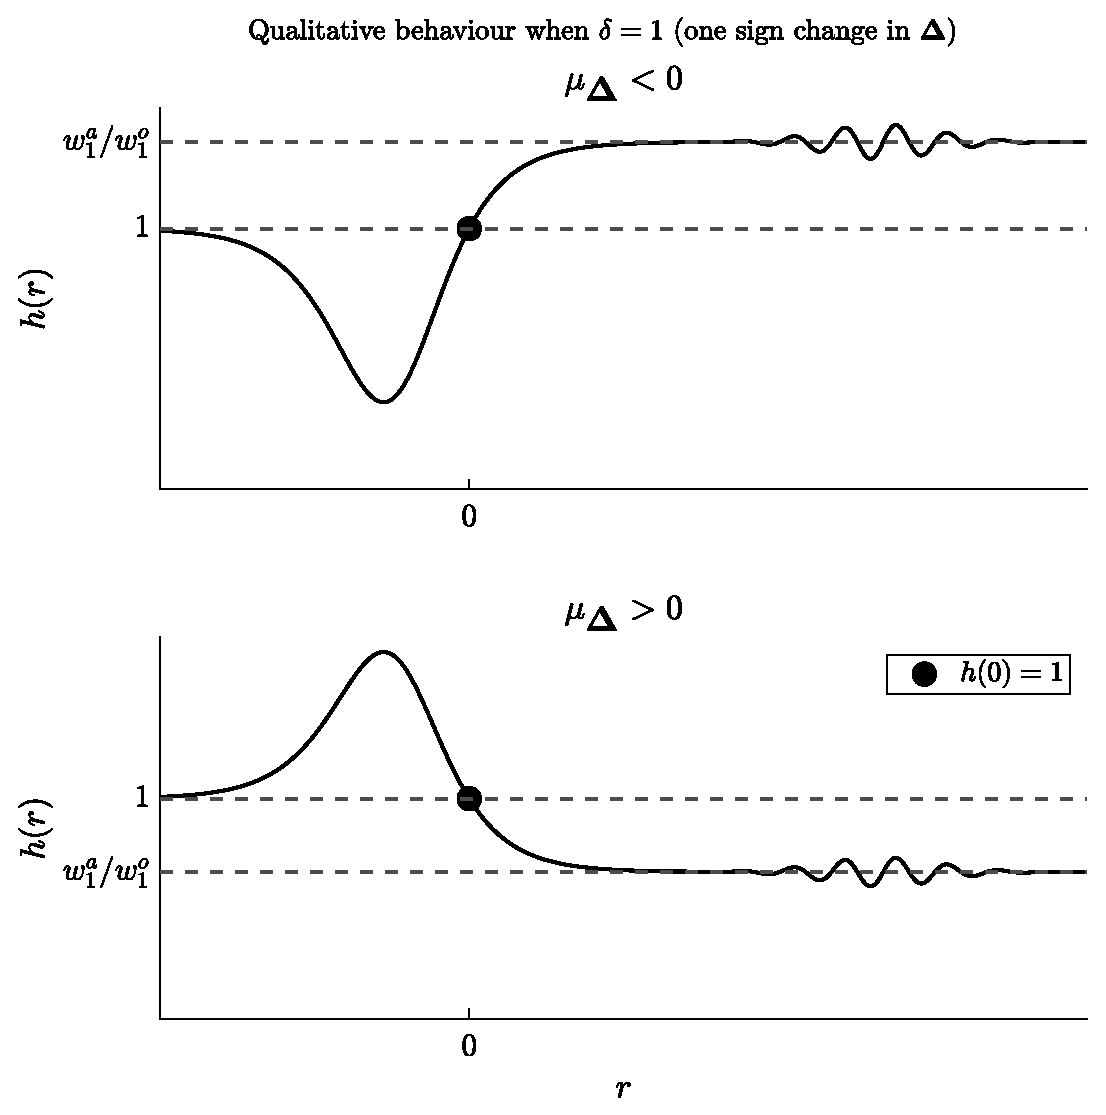
\includegraphics[width=\linewidth]{Figures/Delta_Eq_1_Schematic.eps}
\captionof{figure}{This figure summarises the only two cases when $\delta=1$. When the curve is greater than 1, this illustrates an over-estimate. Conversely, when the curve is less than 1, this illustrates an under-estimate.}
\label{fig:Delta_Eq_1}
\end{minipage}

Figure \ref{fig:Delta_Eq_1_Area} computationally verifies the theory predicted mathematically in Figure \ref{fig:Delta_Eq_1}. We chose a selection of $\boldsymbol{\Delta}$s that varied linearly in $\mu_{\boldsymbol{\Delta}}$ (from 1 to -1), whilst maintaining the condition that $\mu_{\boldsymbol{\Delta}}\cdot \Delta_1 <0$. For details on how we generated these $\boldsymbol{\Delta}$s, see section X. (\textbf{see code section on Notability for details}). The reader should note that there is no significance to the horizontal band on the right hand side sub-figure of Figure \ref{fig:Delta_Eq_1_Area}. This is because this corresponds to $w^a = w^o$, and so there is no difference in inference. Of course, we could have chosen a different family of $\boldsymbol{\Delta}$ such that the mean was 0 but the corresponding $\boldsymbol{\Delta}$ was not $\boldsymbol{0}$. The important features that Figure \ref{fig:Delta_Eq_1_Area} picks up on are:

\begin{enumerate}
    \item The convergence of $h(r)$ to 1 as $r \rightarrow  \infty$ (The difference in inferences seems to tend to zero as $R_t \rightarrow  0^+$.), see right sub-plot.
    \item $h(r)=1$ when $r=0$ ($R_t=1$), see right sub-plot.
    \item The over-estimating of $R_t$ when $\mu_{\boldsymbol{\Delta}}<0$ and under-estimating of $R_t$ when $\mu_{\boldsymbol{\Delta}}>0$
    \end{enumerate}
   
\begin{figure*}
  \centering
  
    \begin{minipage}{\linewidth}
    \centering
    \begin{tikzpicture}[boximg]
      \node (img1) {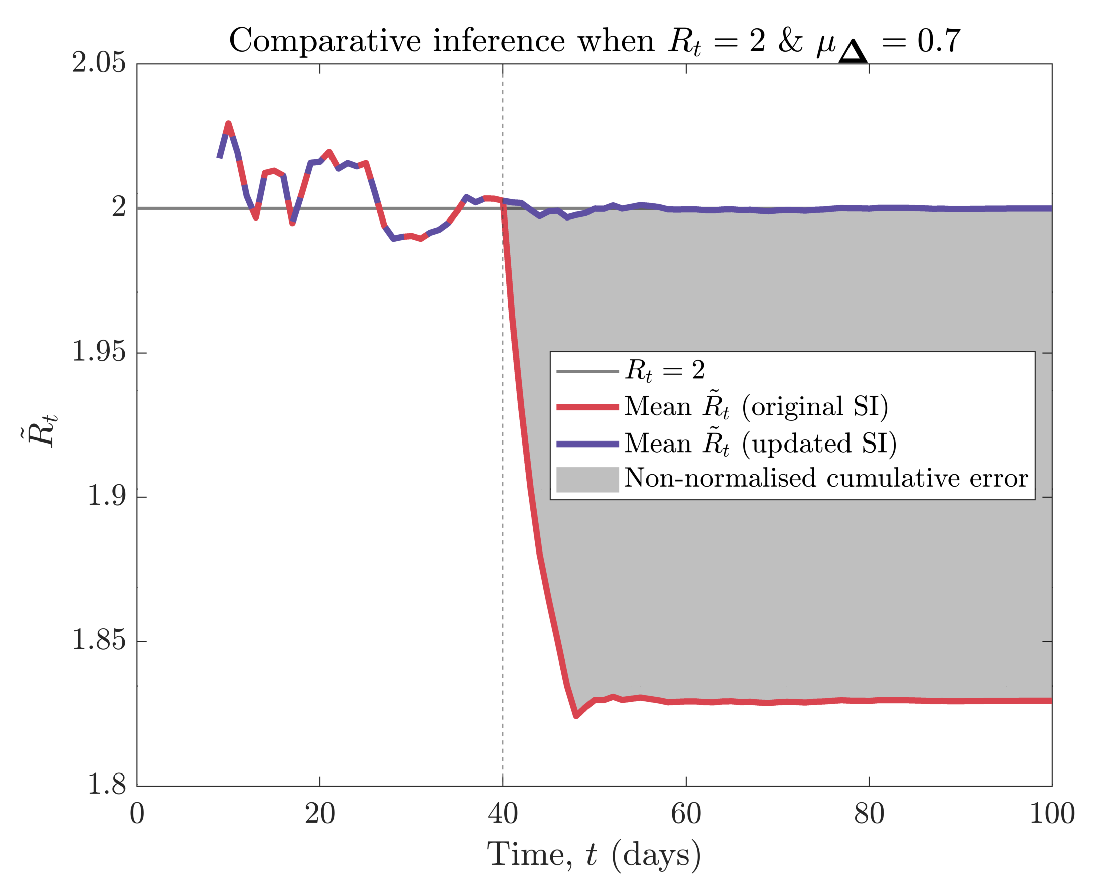
\includegraphics[width=0.3\linewidth]{Figures/Report_Example_1_delta_eq_1.eps}};
      \draw (img1.south west) rectangle (img1.north east);
    \end{tikzpicture}\hfill
  \end{minipage}\\[0.5\baselineskip]
  \begin{minipage}{\linewidth}
    \begin{tikzpicture}[boximg]
      \node[anchor=south west] (img) {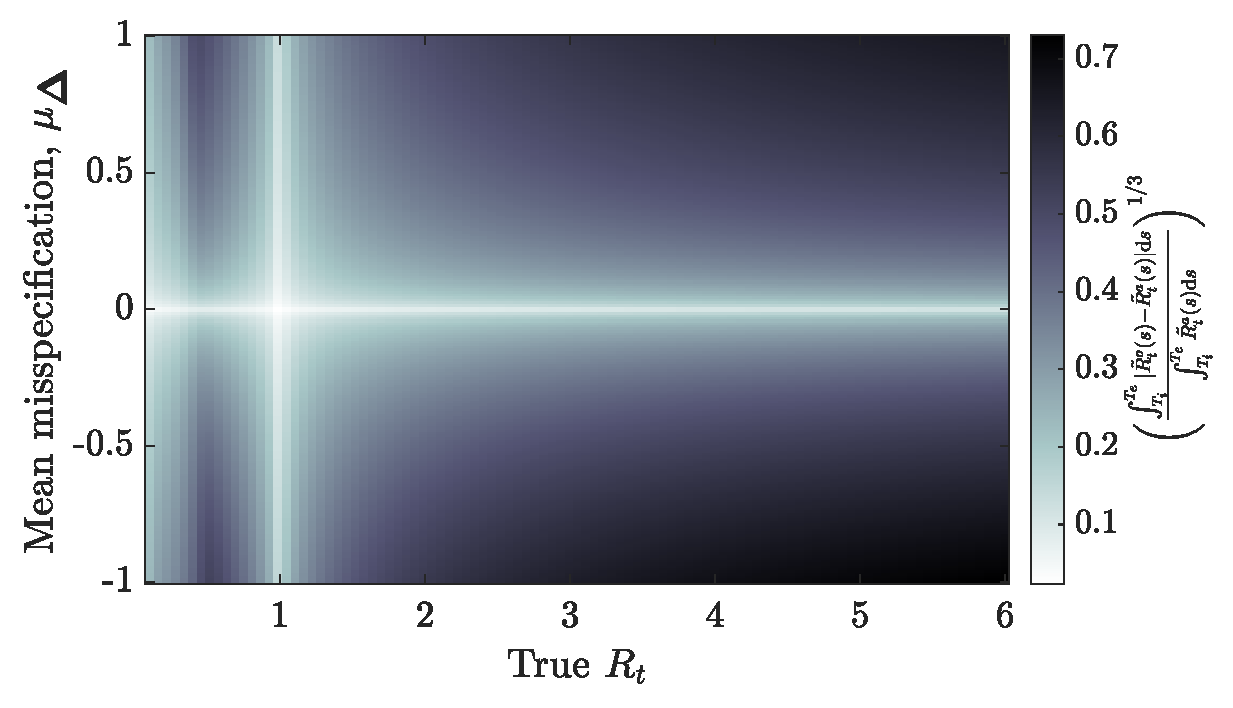
\includegraphics[width=\linewidth]{Figures/Area_R_t_delta_eq_1.eps}};
      \begin{scope}[x=(img.south east),y=(img.north west)]
        \node[draw,minimum height=.163cm,minimum width=0.163cm] (B1) at (0.157,0.8505) {}; %Small red-boxes on main figure:Size in [,] and position in (,)
        \node[draw,minimum height=0.163cm,minimum width=0.163cm] (B3) at (0.325,0.303) {};
      \end{scope}
    \end{tikzpicture}
  \end{minipage}\\[0.5\baselineskip]
  \begin{minipage}{\linewidth}
  \centering
    \begin{tikzpicture}[boximg]
      \node (img3) {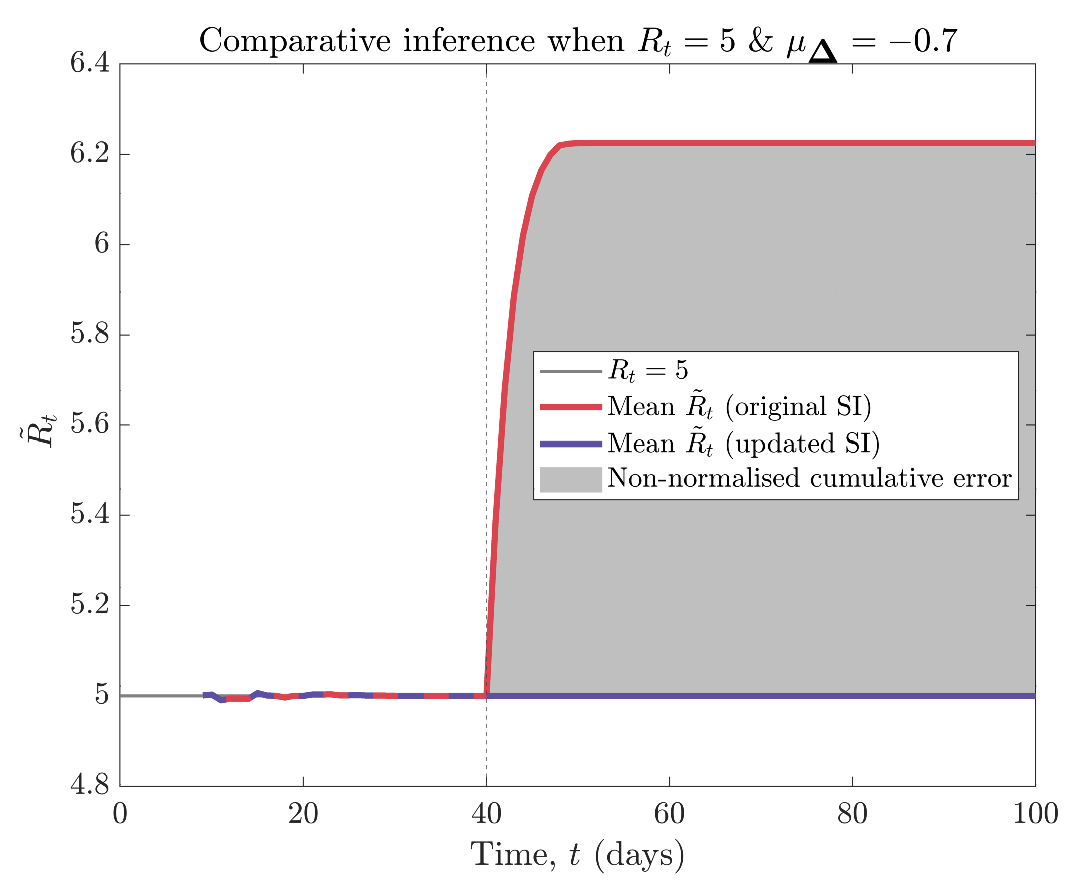
\includegraphics[width=0.3\linewidth]{Figures/Report_Example_2_delta_eq_1.eps}};
      \draw (img3.south west) rectangle (img3.north east);
    \end{tikzpicture}\hfill
  \end{minipage}
  \begin{tikzpicture}[overlay,boximg]
    \draw (B1) -- (img1);
    \draw (B3) -- (img3);
  \end{tikzpicture}
  \caption{The National Gallery of Canada}
\end{figure*}

\begin{figure*}
  \centering
  
    \begin{minipage}{\linewidth}
    \centering
    \begin{tikzpicture}[boximg]
      \node (img1) {\includegraphics[width=0.3\linewidth]{example-image-10x16}};
      \draw (img1.south west) rectangle (img1.north east);
    \end{tikzpicture}\hfill
    \begin{tikzpicture}[boximg]
      \node (img2) {\includegraphics[width=0.3\linewidth]{example-image-10x16}};
      \draw (img2.south west) rectangle (img2.north east);
    \end{tikzpicture}\hfill
  \end{minipage}\\[0.5\baselineskip]
  \begin{minipage}{\linewidth}
    \begin{tikzpicture}[boximg]
      \node[anchor=south west] (img) {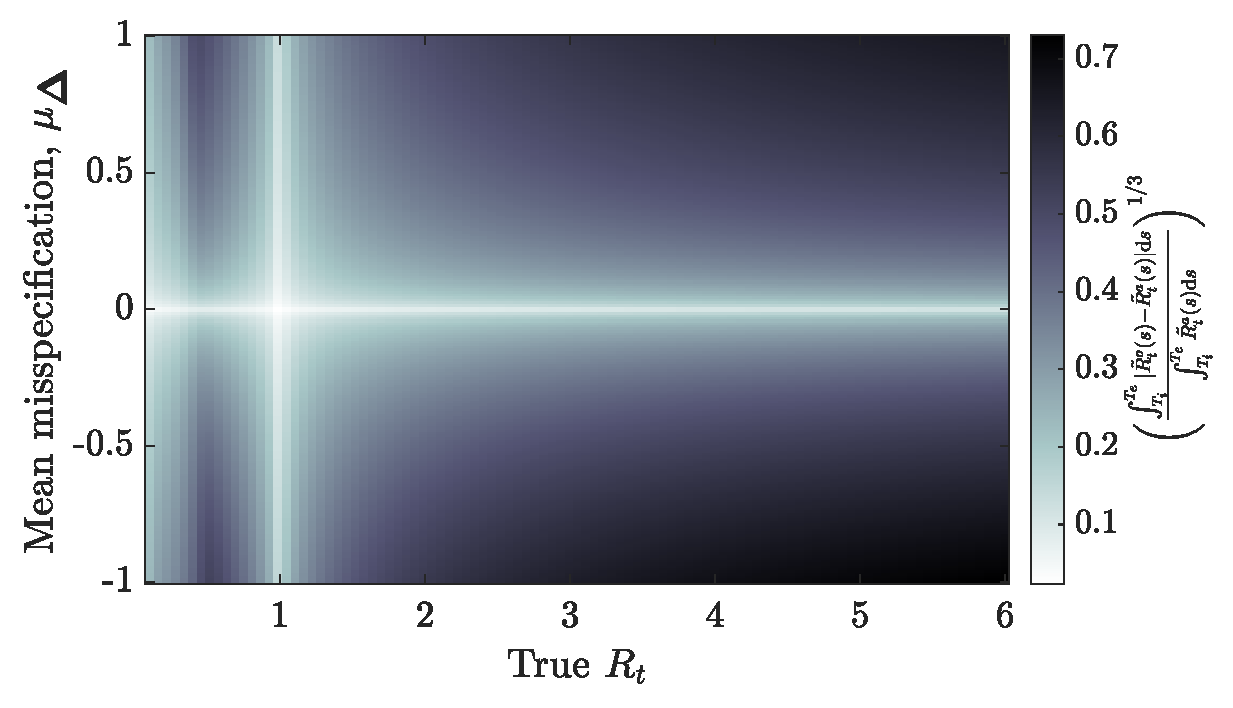
\includegraphics[width=\linewidth]{Figures/Area_R_t_delta_eq_1.eps}};
      \begin{scope}[x=(img.south east),y=(img.north west)]
        \node[draw,minimum height=.6cm,minimum width=1.00cm] (B1) at (0.5,0.60) {}; %Small red-boxes on main figure:Size in [,] and position in (,)
        \node[draw,minimum height=0.8cm,minimum width=0.50cm] (B2) at (0.7,0.25) {};
        \node[draw,minimum height=0.8cm,minimum width=0.50cm] (B3) at (0.1,0.25) {};
      \end{scope}
    \end{tikzpicture}
    \caption{}
  \end{minipage}\\[0.5\baselineskip]
  \begin{minipage}{\linewidth}
    \begin{tikzpicture}[boximg]
      \node (img3) {\includegraphics[width=0.3\linewidth]{example-image-10x16}};
      \draw (img3.south west) rectangle (img3.north east);
    \end{tikzpicture}\hfill
  \end{minipage}
  \begin{tikzpicture}[overlay,boximg]
    \draw (B1) -- (img1);
    \draw (B2) -- (img2);
    \draw (B3) -- (img3);
  \end{tikzpicture}
  \caption{The National Gallery of Canada}
\end{figure*}

The diagram shows that if we are able to prove that in the real world, $\delta=1$, we can make concrete assertions about whether we are over/under-estimating $R_t$.\\

Unfortunately, the consequences when $\delta=2$ is marginally more mathematically complex which means the real-world consequences for $R_t$ estimation when $\delta=2$ are difficult to summarise. In short, it is no longer so obvious whether or not we have over/under-estimated $R_t$. As opposed to when $\delta=1$, there are now 4 cases (combinations of $\mu_{\boldsymbol{\Delta}} \lessgtr 0$ and $\Delta_1 \lessgtr 0$) to consider for the shape of $h(r)$ (since we can no longer eliminate two of the cases as we could previously). Rather than summarising what this means for the over/under-estimates, we refer the reader to Figure \ref{fig:Delta_Eq_2}.

\begin{figure*}
\centering
\includegraphics[width=\linewidth]{Figures/Delta_Eq_2_Schematic.eps}
\captionof{figure}{Unlike the case when $\delta=1$, there is no implication for $\mu_{\boldsymbol{\Delta}}$ when $\Delta_1$ takes a particular sign (or vice versa). This implies that there are 4 cases to consider instead of 2. Similarly, the curve being greater or less than 1 indicates an over/under-estimate respectively.}
\label{fig:Delta_Eq_2}
\end{figure*}



\subsubsection{Shape of $h(c)$ local to $c=0$}
We recall that 
\begin{align*}
L'(x) &= -\sum_{i=1}^{N}e^{-ix}iw_i \\
\implies L''(x) &= \sum_{i=1}^{N}e^{-ix}i^2w_i
\end{align*}
We can deduce that $L'(0) = -\mathbb{E}[\boldsymbol{w}]$ and $L''(0) = \mathrm{Var}[\boldsymbol{w}]+\mathbb{E}[\boldsymbol{w}]^2$.\\
The quotient rule and the repeated quotient rule say that
\begin{align*}
&\text{if }
    h(x)&&= \frac{f(x)}{g(x)} \text{,}\\
    &\text{then }
    h'(x)&&= \frac{f'(x)g(x) - f(x)g'(x)}{g^2(x)}\\
    &\text{and }
    h''(x)&&= \frac{f''(x)g(x)-f(x)g''(x)}{g^4(x)}
\end{align*}

As will become clear, we only need to be concerned about the \textit{sign} of the first and second derivative of $h$ at $c=0$. Since both $g^2(x)>0 \forall x$ and $g^4(x)>0 \forall x$ we only need to consider the numerator.

\begin{align*}
\mathrm{sgn} \{ h'(c)\} &= \mathrm{sgn} \{\Large[qte^{ct}L_a(c) +qe^{ct}L_a'(c)\Large] \cdot \Large[ p+q e^ct L_o(c) \Large] \\ 
&- \Large[qte^{ct}L_o(c) +qe^{ct}L_o'(c)\Large] \cdot \Large[ p+q e^ct L_a(c) \Large] \}\\
\implies \mathrm{sgn} \{ h'(0)\}&= \mathrm{sgn} \{qL_a'(0)(p+q)-qL_o(o)(p+q) \}\\
&= \mathrm{sgn} \{ q(p+q)\Large( L_a'(0) - L_o'(0)\Large) \}\\
&= \mathrm{sgn} \{ q(p+q)(\mu_o-\mu_a) \}
\end{align*}

\begin{equation*}
\begin{split}
\mathrm{sgn} \{ h''(c)\} &= \mathrm{sgn} \{\Large[ qe^{ct}L_a(c)+qt^2e^{ct}L_a(c)\\
&+ qte^{ct}L_a'(c)+qe^{ct}L_a''(c) \Large] \cdot \Large[(p+qe^{ct}L_o(c) \Large]\\ 
&- \Large[ qe^{ct}L_o(c)+qt^2e^{ct}L_o(c)\\
&+ qte^{ct}L_o'(c)+qe^{ct}L_o''(c) \Large] \cdot \Large[p+qe^{ct}L_a(c) \Large] \} \\
\implies \mathrm{sgn} \{ h''(0)\}&= \mathrm{sgn} \{q(p+q)\{ \Large(1+ \mu_a^2 +\sigma_a^2 \Large) - \Large( 1+ \mu_o^2 +\sigma_o^2 \Large) \}\\
&= \mathrm{sgn} \{q(p+q)(\mu^2_a-\mu_o^2 + \sigma_a^2 -\sigma_o^2) \}
\end{split}
\end{equation*}

Now we are equipped with both the sign of $h'(0)$ and $h''(0)$, as well as how many zeros $h(c)$ has. We also know the behaviour of $h(c)$ as $c \rightarrow \pm \infty$.\\
When it comes to sketching $h(c)$ (which is critical to determining how divergent $\tilde{R}_t^o$ is to $\tilde{R}_t^a$), it turns out that only $\delta$ and $\mu_d$ ($\mu_a- \mu_o$) are the important factors. There is of course the unusual case where $\mu_d=0$, in which case $\mathrm{Var}(\Delta)$ becomes important once again.

For example, if 
\begin{enumerate}
    \item $\boldsymbol{\Delta}$ has one sign change
    \item $\mu_a =\mu_o$
    \item $\sigma_a > \sigma_o$,
\end{enumerate}
then $h(c)>1 \forall c \ne 0$, i.e. we will always over-estimate the true $R_t$, unless $R_t = 1$ ($c=0$).\\
\textbf{To do: Continue writing up proof, explain that v(c) all `scale' the same and are `co-linear'. Then use this to show that c=0 is the only solution for R/R =1. This is the base line for proving the rest of the results.}


\textbf{To do: Talk about how in the method the incidence data needs to be from when the symptoms onset????}

\subsection{Analytical calculation of $\Delta$ for computational work, i.e. derivation of}

The following derivations make use of the finite sums of powers of natural numbers (which can be looked up in page 2 of \cite{Gradshteyn-Ryzhik-0}).

Equation \ref{eq:cons_of_prob_1} indicates that

\begin{align*}
    a_j + b_j + 2a_j + b_j + \cdots Na_j + b_j &= 0 \forall j = 1, \cdots , M \\
    \implies \frac{N}{2}(N+1)a_j + Nb_j &= 0 \forall j =1, \cdots , M,
\end{align*}
whilst equation \ref{eq:mean_1} indicates in a similar fashion that

\begin{align*}
    a_j + b_j + 2(2a_j+b_j) + \cdots N(Na_j + b_j) &= \mu_j \forall j = 1, \cdots , M \\
    \implies \frac{N}{6}(N+1)(2N+1)a_j + \frac{N}{2}(N+1)b_j &= \mu_j \forall j =1, \cdots , M,
\end{align*}

This means that 
\begin{align*}
\begin{pmatrix}
    N+1 & 2\\
    2N+1 & 3
    \end{pmatrix}
    \begin{pmatrix}
    a_j\\
    b_j
    \end{pmatrix}
    &= \begin{pmatrix}
    \frac{6\mu_j}{N(N+1)}\\
    0
    \end{pmatrix} \forall j = 1, \cdots ,M
\end{align*}

We can invert the above matrix (it is only singular when $N=1$!) to solve for $a_j$ and $b_j$. We can go one step further in choosing to package the above matrix into the larger matrix $\boldsymbol{B}_q$ which enables all $a_j$ and $b_j$ to be found in one computation.\\

The derivation of \textbf{equation} takes a similar path. The analogous equations to 

\begin{figure*}
\centering
\includegraphics[width=\linewidth]{Figures/Hybrid_Progression.eps}
\captionof{figure}{Method of transitioning between `old' and `actual' serial intervals. \textbf{Is this graph as clear as it could be? Could just change the colour of the black line to correspond to contributions.}}
\label{fig:Hybrid_Progression}
\end{figure*}
\bibliography{References.bib}
\bibliographystyle{ieeetr}

\end{document}